%%%%%%%%%%%%%%%%%%%%%%%%%%%%%%%%%%%%%%%%
% Masters/Doctoral Thesis 
% LaTeX Template
% Version 2.4 (22/11/16)
%
% This template has been downloaded from:
% http://www.LaTeXTemplates.com
%
% Version 2.x major modifications by:
% Vel (vel@latextemplates.com)
%
% This template is based on a template by:
% Steve Gunn (http://users.ecs.soton.ac.uk/srg/softwaretools/document/templates/)
% Sunil Patel (http://www.sunilpatel.co.uk/thesis-template/)
%
% Template license:
% CC BY-NC-SA 3.0 (http://creativecommons.org/licenses/by-nc-sa/3.0/)
%
%%%%%%%%%%%%%%%%%%%%%%%%%%%%%%%%%%%%%%%%%

%----------------------------------------------------------------------------------------
%	THESIS TEMPLATE CONFIGURATION
%----------------------------------------------------------------------------------------

\documentclass[
11pt, % The default document font size, options: 10pt, 11pt, 12pt
%oneside, % Two side (alternating margins) for binding by default, uncomment to switch to one side
english, % ngerman for German
singlespacing, % Single line spacing, alternatives: onehalfspacing or doublespacing
%doublespacing
%draft, % Uncomment to enable draft mode (no pictures, no links, overfull hboxes indicated)
nolistspacing, % If the document is onehalfspacing or doublespacing, uncomment this to set spacing in lists to single
liststotoc, % Uncomment to add the list of figures/tables/etc to the table of contents
toctotoc, % Uncomment to add the main table of contents to the table of contents
parskip, % Uncomment to add space between paragraphs
%nohyperref, % Uncomment to not load the hyperref package
headsepline, % Uncomment to get a line under the header
%chapterinoneline, % Uncomment to place the chapter title next to the number on one line
consistentlayout, % Uncomment to change the layout of the declaration, abstract and acknowledgements pages to match the default layout
]{MastersDoctoralThesis} % The class file specifying the document structure

%----------------------------------------------------------------------------------------
%	Preamble: Font / Language
%----------------------------------------------------------------------------------------

\usepackage[utf8]{inputenc} % Required for inputting international characters
\usepackage[T1]{fontenc} % Output font encoding for international characters
\usepackage{palatino} % Use the Palatino font by default

\usepackage{lscape}	

%%%%
% Chineses package
%%%%
\usepackage{CJKutf8}			 

%\newcommand{\dojapanese}[1]{%
%   \begin{CJK}{UTF8}{}\begin{Japanese}#1\end{Japanese}\end{CJK}%
%}


%%%%
%% Japanese package %%
%%%%%
\newenvironment{Japanese}{%
\CJKfamily{min}%
\CJKtilde
\CJKnospace}{}

\newcommand{\dojapanese}[1]{%
   \begin{CJK}{UTF8}{}\begin{Japanese}#1\end{Japanese}\end{CJK}%
}


%----------------------------------------------------------------------------------------
%	Preamble: Paragraph, TOC
%----------------------------------------------------------------------------------------
 
\setlength{\parindent}{5mm}
\setcounter{tocdepth}{2} % chapter / section / subsection in TOC

% item prevent page break
\makeatletter 
\newcommand\mynobreakpar{\par\nobreak\@afterheading} 
\makeatother

%----------------------------------------------------------------------------------------
%	Preamble: Page number
%----------------------------------------------------------------------------------------

\usepackage{calc} %for counting page number


%----------------------------------------------------------------------------------------
%	Preamble: Mathematics 
%----------------------------------------------------------------------------------------

\usepackage{amsmath} % math package
\usepackage{amssymb} % math symbol
\usepackage{siunitx} % SI unit package. \SI{ number }{ unit }
\usepackage{braket} %braket

%----------------------------------------------------------------------------------------
%	Preamble: Table 
%----------------------------------------------------------------------------------------

\usepackage{xcolor,colortbl}
\usepackage{etoolbox} % color table
\definecolor{Gray}{gray}{0.85}
\definecolor{LightCyan}{rgb}{0.88,1,1}

\newcommand{\mc}[2]{\multicolumn{#1}{c}{#2}}
\newcolumntype{a}{>{\columncolor{Gray}}l}
\newcolumntype{b}{>{\columncolor{Gray}}c}

\newcommand{\dtoprule}{\specialrule{1pt}{0pt}{0.4pt}%
            \specialrule{0.3pt}{0pt}{\belowrulesep}%
            }
\newcommand{\dbottomrule}{\specialrule{0.3pt}{0pt}{0.4pt}%
            \specialrule{1pt}{0pt}{\belowrulesep}%
            }
%\renewcommand\arraystretch{1.5} % add extra space between rows
\usepackage{makecell}

%----------------------------------------------------------------------------------------
%	Preamgle: Figure
%----------------------------------------------------------------------------------------

% side caption
%\usepackage[capbesideposition={bottom,outside},facing=yes,capbesidesep=quad]{floatrow}
%\usepackage[capbesideposition={center,outside}]{floatrow}
\usepackage{rotating}
\usepackage{sidecap}
\usepackage{caption}
\usepackage{subcaption}
\captionsetup{justification = raggedright, singlelinecheck=true}
%\renewcommand\arraystretch{1.5}

% figure option [H]
\usepackage{float}

%----------------------------------------------------------------------------------------
%	Preamble: math in title is set to be bold.
%----------------------------------------------------------------------------------------
\makeatletter
\g@addto@macro\bfseries{\boldmath}
\makeatother

%----------------------------------------------------------------------------------------
%	Preamble: Biblatex
%----------------------------------------------------------------------------------------
\usepackage[backend=biber,sorting=none, style=numeric,natbib=true, url = false]{biblatex} % Use the bibtex backend with the authoryear citation style (which resembles APA)
\setlength\bibitemsep{0.8\baselineskip} % set the spacing between references
\addbibresource{thesis.bib} % The filename of the bibliography
\usepackage[autostyle=true]{csquotes} % Required to generate language-dependent quotes in the bibliography

% go back hyperlink option
%\renewbibmacro*{pageref}{%
%  \printtext[parens]{%
%    \Acrobatmenu{GoBack}{Go back}%
%  }%
%}

%----------------------------------------------------------------------------------------
%	Preamble: Index setting
%----------------------------------------------------------------------------------------
%\begin{filecontents*}{\jobname.mst}
%headings_flag 1
%heading_prefix "{\\textbf{"
%heading_suffix "}}\\nopagebreak\n"
%\end{filecontents*}

\usepackage{makeidx}			 % index package
\usepackage[totoc]{idxlayout} % Create index in the table of contents

\makeindex

%----------------------------------------------------------------------------------------
%	Preamble: others
%----------------------------------------------------------------------------------------

% random paragraph
\usepackage{lipsum}

%----------------------------------------------------------------------------------------
%	MARGIN SETTINGS
%----------------------------------------------------------------------------------------

\geometry{
	paper=a4paper, % Change to letterpaper for US letter
	inner=3  cm, % Inner margin
	outer=2.5cm, % Outer margin
	bindingoffset=.5cm, % Binding offset
	top=1.5cm, % Top margin
	bottom=1.5cm, % Bottom margin
	%showframe, % Uncomment to show how the type block is set on the page
}

%----------------------------------------------------------------------------------------
%	THESIS INFORMATION
%----------------------------------------------------------------------------------------

\thesistitle{Study of $K_L^0 \to \pi^0 \nu \bar{\nu}$ and $K_L^0 \to \pi^0 \gamma \gamma$ with Cluster-Finding Trigger at KOTO} % Your thesis title, this is used in the title and abstract, print it elsewhere with \ttitle
\supervisor{Dr. Yee Bob \textsc{Hsiung}} % Your supervisor's name, this is used in the title page, print it elsewhere with \supname
\examiner{} % Your examiner's name, this is not currently used anywhere in the template, print it elsewhere with \examname
\degree{Doctor of Philosophy} % Your degree name, this is used in the title page and abstract, print it elsewhere with \degreename
\author{Chieh Lin} % Your name, this is used in the title page and abstract, print it elsewhere with \authorname
\addresses{} % Your address, this is not currently used anywhere in the template, print it elsewhere with \addressname

\subject{Physics} % Your subject area, this is not currently used anywhere in the template, print it elsewhere with \subjectname
\keywords{haha,haha} % Keywords for your thesis, this is not currently used anywhere in the template, print it elsewhere with \keywordnames
\university{\href{http://www.ntu.edu.tw}{National Taiwan University}} % Your university's name and URL, this is used in the title page and abstract, print it elsewhere with \univname
\department{\href{http://www.phys.ntu.edu.tw}{Department or Physics}} % Your department's name and URL, this is used in the title page and abstract, print it elsewhere with \deptname
\group{\href{http://researchgroup.university.com}{High energy physics}} % Your research group's name and URL, this is used in the title page, print it elsewhere with \groupname
%\faculty{\href{http://faculty.university.com}{Faculty Name}} % Your faculty's name and URL, this is used in the title page and abstract, print it elsewhere with \facname

\AtBeginDocument{
\hypersetup{pdftitle=\ttitle} % Set the PDF's title to your title
\hypersetup{pdfauthor=\authorname} % Set the PDF's author to your name
\hypersetup{pdfkeywords=\keywordnames} % Set the PDF's keywords to your keywords
}

\begin{document}

\frontmatter % Use roman page numbering style (i, ii, iii, iv...) for the pre-content pages

\pagestyle{plain} % Default to the plain heading style until the thesis style is called for the body content


%----------------------------------------------------------------------------------------
%	Title (NTU requirement, softcover version)
%----------------------------------------------------------------------------------------

%\thispagestyle{empty}

%\begin{titlepage}

%\parskip=8pt					%space btw paragraphs
%\linespread{1.5}

%\begin{center}

%\thispagestyle{empty}

%\begin{center}
%\begin{CJK}{UTF8}{bkai}
% \vspace {4.0cm}
%\LARGE \noindent   國立臺灣大學 理學院物理學研究所 \\
%        \vspace {0.0cm}
%        博士學位論文\\
%            \end{CJK}
%            \vspace {0.2cm}
%{
%    \noindent
%        \large Graduate Institute of Physics\\
%        \vspace {0.0cm}
%    \large College of Science\\
%        \vspace {0.0cm}
%    \large National Taiwan University\\
%        \vspace {0.0cm}
%    \large Doctoral Dissertation \\
%}

%\vspace {2.0cm}
%\setlength{\baselineskip}{32pt}
%\begin{CJK}{UTF8}{bkai}
%\LARGE  \noindent   
%在KOTO實驗中利用電磁雨簇計數的觸發系統測量\\中性K介子的稀有衰變
%\end{CJK}

%\vspace {0.5cm}
%\setlength{\baselineskip}{24pt}
%{\LARGE \noindent Study of the Rare Kaon Decays $K_L^0 \to \pi^0 \nu \bar{\nu}$ and $K_L^0 \to \pi^0 \gamma \gamma$ with the Cluster-Finding Trigger at the J-PARC KOTO Experiment
%}\\

%\vspace {5.0cm}

%\begin{CJK}{UTF8}{bkai}
%\Large \noindent   林  杰 \\
%\vspace {0.0cm}
%\Large Chieh Lin\\
%\vspace {0.2cm}
%\Large 指導教授:熊怡 教授\\
%\vspace {0.0cm}
%\Large Advisor : Prof. Yee Bob Hsiung\\

%\vspace {0.4cm}
%\Large \noindent   中華民國110年1月\\
%\Large \noindent   January, 2021\\
%\end{CJK}

%\end{center}

%\end{center}

%\end{titlepage}

%\thispagestyle{empty}
%~\\
%\cleardoublepage


%----------------------------------------------------------------------------------------
%	Title page (Main title, hardcover version)
%----------------------------------------------------------------------------------------

\begin{titlepage}
\begin{center}

\vspace*{.06\textheight}
{\scshape\LARGE \univname\par}\vspace{1.5cm} % University name
\textsc{\Large Doctoral Thesis}\\[0.5cm] % Thesis type

\HRule \\[0.4cm] % Horizontal line
{\huge \bfseries {Study of $K_L^0\to\pi^0\nu\overline{\nu}$ and $K_L^0\to\pi^0\gamma\gamma$ \\ with Cluster-Finding Trigger at KOTO} \par}\vspace{0.4cm} % Thesis title
\HRule \\[1.5cm] % Horizontal line
 
\begin{minipage}[t]{0.4\textwidth}
\begin{flushleft} \large
\emph{Author:}\\
\href{http://www.johnsmith.com}{\authorname} % Author name - remove the \href bracket to remove the link
\end{flushleft}
\end{minipage}
\begin{minipage}[t]{0.4\textwidth}
\begin{flushright} \large
\emph{Supervisor:} \\
\href{http://www.jamessmith.com}{\supname} % Supervisor name - remove the \href bracket to remove the link  
\end{flushright}
\end{minipage}\\[3cm]
 
\vfill

\large \textit{A thesis submitted in fulfillment of the requirements\\ for the degree of \degreename}\\[0.3cm] % University requirement text
\textit{in the}\\[0.4cm]
\groupname\\\deptname\\[2cm] % Research group name and department name
 
\vfill

{\large \today}\\[4cm] % Date
%\includegraphics{Logo} % University/department logo - uncomment to place it
 
\vfill
\end{center}
\end{titlepage}


%\thispagestyle{empty}

%\begin{titlepage}
%\begin{center}

%\vspace*{.06\textheight}
%{\scshape\LARGE \univname\par}\vspace{1.5cm} % University name
%\textsc{\Large Doctoral Dissertation}\\[0.5cm] % Thesis type

%\HRule \\[0.4cm] % Horizontal line
%{\LARGE %\bfseries 
%Study of $K_L^0 \to \pi^0 \nu \bar{\nu}$ and $K_L^0 \to \pi^0 \gamma \gamma$ \\ with Cluster-Finding Trigger at KOTO
%\\ }\vspace{0.4cm} % Thesis title
%\HRule \\[1.5cm] % Horizontal line
 
%\begin{minipage}[t]{0.4\textwidth}
%\begin{flushleft} \Large
%\emph{Author:}\\
%\authorname
%\href{http://www.johnsmith.com}{\authorname} % Author name - remove the \href bracket to remove the link
%\authorname
%\end{flushleft}

%\end{minipage}
%\begin{minipage}[t]{0.4\textwidth}
%\begin{flushright} \Large
%\emph{Supervisor:} \\
%\supname
%\href{http://www.jamessmith.com}{\supname} % Supervisor name - remove the \href bracket to remove the link  
%\end{flushright}
%\end{minipage}\\[3cm]
 
%\vspace{7 cm}
 
%\begin{center}
%
\includegraphics[scale=0.5]{NTU.jpg}
%\end{center}  

%\vspace{1 cm} 
 
%{\Large \today}\\[4cm] % Research group name and department name 
 
%\vfill 
 
%\end{center}
%\end{titlepage}



%----------------------------------------------------------------------------------------
%	Title page (2nd title page)
%----------------------------------------------------------------------------------------

\thispagestyle{empty}

\begin{titlepage}
\begin{center}

\vspace*{.06\textheight}
{\scshape\LARGE \univname\par}\vspace{1.5cm} % University name
\textsc{\Large Doctoral Dissertation}\\[0.5cm] % Thesis type

\HRule \\[0.4cm] % Horizontal line
{\LARGE %\bfseries 
Study of $K_L^0 \to \pi^0 \nu \bar{\nu}$ and $K_L^0 \to \pi^0 \gamma \gamma$ with Cluster-Finding Trigger at KOTO
\\ }\vspace{0.4cm} % Thesis title
\HRule \\[1.5cm] % Horizontal line
 
\begin{minipage}[t]{0.4\textwidth}
\begin{flushleft} \Large
\emph{Author:}\\
\href{http://www.johnsmith.com}{\authorname} % Author name - remove the \href bracket to remove the link
%\authorname
\end{flushleft}

\end{minipage}
\begin{minipage}[t]{0.4\textwidth}
\begin{flushright} \Large
\emph{Supervisor:} \\
%\supname
\href{http://www.jamessmith.com}{\supname} % Supervisor name - remove the \href bracket to remove the link  
\end{flushright}
\end{minipage}\\[3cm]
 
%\vspace{4 cm}
 
\begin{center}

\includegraphics[scale=0.5]{NTU.jpg}
\end{center}  

\vspace{1 cm} 
 
{\Large \today}\\[4cm] % Research group name and department name 
 
\vfill 
 
\end{center}
\end{titlepage}

\linespread{0}




% copyright note
\clearpage
\vspace*{130mm}
\begin{center}
{% begin group
   \thispagestyle{empty}
   %\footnotesize\itshape
   \setlength{\parskip}{\baselineskip}
   \setlength{\parindent}{0pt}
      
   \copyright\,2021, by Chieh Lin \\
   jay@hep1.phys.ntu.edu.tw \\
   ALL RIGHTS RESERVED 
}% end group
\end{center}


\clearpage

%----------------------------------------------------------------------------------------
%	口試委員審定書
%----------------------------------------------------------------------------------------

\pagenumbering{roman}
%\addtocounter{page}{-1}

\begin{CJK}{UTF8}{bkai}
 ~ \\
 ~ \\
 ~ \\
\Large \textbf{口試委員審定書 Doctoral Committee}
\end{CJK}

%\begin{figure*}[t]
%\begin{center}
%\hspace*{-3.2cm}
%\includegraphics[scale=1.0]{committee_list.pdf}
%\label{defense_proof}
%\end{center}
%\end{figure*}
\addchaptertocentry{Approval}
\cleardoublepage
\cleardoublepage


%----------------------------------------------------------------------------------------
%	Authorship
%----------------------------------------------------------------------------------------

\begin{declaration}
\addchaptertocentry{\authorshipname} % Add the declaration to the table of contents

\noindent I, \authorname, declare that this thesis titled, \enquote{\ttitle} and the work presented in it are my own. I confirm that:

\begin{itemize} 
\item This work was done wholly or mainly while in candidature for a research degree at this University.
\item Where any part of this thesis has previously been submitted for a degree or any other qualification at this University or any other institution, this has been clearly stated.
\item Where I have consulted the published work of others, this is always clearly attributed.
\item Where I have quoted from the work of others, the source is always given. With the exception of such quotations, this thesis is entirely my own work.
\item I have acknowledged all main sources of help.
\item Where the thesis is based on work done by myself jointly with others, I have made clear exactly what was done by others and what I have contributed myself.
\end{itemize}

\vfill 
 
\noindent Signed:\\
\rule[0.5em]{25em}{0.5pt} % This prints a line for the signature
 
\noindent Date:\\
\rule[0.5em]{25em}{0.5pt} % This prints a line to write the date
\end{declaration}

\cleardoublepage

%----------------------------------------------------------------------------------------
%	中文摘要
%----------------------------------------------------------------------------------------

\begin{CJK}{UTF8}{bkai}
 ~ \\
 ~ \\
 ~ \\
\huge \textbf{中文摘要}
\end{CJK}

\vspace{1.5cm}

\begin{CJK}{UTF8}{bkai}
論文包含三個主題:KOTO觸發系統.
KOTO的取數利用利用資料渠道的方式,
\end{CJK}

\vspace{0.5cm}

%\begin{CJK}{UTF8}{bkai}
%第三個主題是台大高能實驗室參與Belle II第一階中央飄移室觸發系統的研究,在此系統中,Merger電路板負責簡化從前端讀出板的資料,再傳送到後段的帶電粒子軌跡重建模組,關於Merger電路板各方面的設計將在論文中詳細描述。台大團隊發展了自定義的光纖傳輸通訊協定,使用於在中央飄移室觸發系統的資料流之中,亦發展了整體系統的流量控制與資料同步的方式,論文中也會提到此通訊協定的發展與應用的細節。
%\end{CJK}

\vspace{0.5cm}

\begin{CJK}{UTF8}{bkai}
\textbf{關鍵詞}:觸發系統,K介子.稀有衰變,CP對稱破壞
\end{CJK}

\linespread{0}

\begin{CJK}{UTF8}{bkai}
\addchaptertocentry{中文摘要}
\clearpage
\end{CJK}

%----------------------------------------------------------------------------------------
%	ABSTRACT
%----------------------------------------------------------------------------------------

\begin{abstract}
\addchaptertocentry{\abstractname} % Add the abstract to the table of contents
Click on "Project" in the top bar, which will expose the files associated with the project in a tree on the left. The click on MastersDoctoralThesis.cls. 
\par
In that file you should be able to see what I show above. If it is not visible, then the project you shared may have been altered and you should start anew
\par
\vspace{0.5cm}
\textbf{Keywords}: haha, hbhb, hchch.
\end{abstract}

\setcounter{page}{7}

%----------------------------------------------------------------------------------------
%	ACKNOWLEDGEMENTS
%----------------------------------------------------------------------------------------
\begin{acknowledgements}
\addchaptertocentry{\acknowledgementname} % Add the acknowledgements to the table of contents
The acknowledgments and the people to thank go here, don't forget to include your project advisor\ldots
\end{acknowledgements}

\cleardoublepage

%----------------------------------------------------------------------------------------
%	PREFACE
%----------------------------------------------------------------------------------------
%
\chapter*{Preface}
\addchaptertocentry{Preface}

This is preface.

\cleardoublepage


%----------------------------------------------------------------------------------------
%	LIST OF CONTENTS/FIGURES/TABLES PAGES
%----------------------------------------------------------------------------------------
\begin{CJK}{UTF8}{bkai}
\tableofcontents % Prints the main table of contents
\end{CJK}

\listoffigures % Prints the list of figures

\listoftables % Prints the list of tables

%----------------------------------------------------------------------------------------
%	ABBREVIATIONS
%----------------------------------------------------------------------------------------

\begin{abbreviations}{ll} % Include a list of abbreviations (a table of two columns)

%% CDT
\textbf{CDT} & \textbf{C}lock \textbf{D}istribution and \textbf{T}rigger Processor\\

\textbf{CKM} & \textbf{C}abibbo-\textbf{K}obayashi-\textbf{M}askawa \\

%% DAQ
\textbf{DAQ} & \textbf{D}ata \textbf{A}c\textbf{Q}usition System \\

%% FADC
\textbf{FADC} & \textbf{F}lush-\textbf{A}nalog-to-\textbf{D}igitized \textbf{C}onverter \\

%% FCNC
\textbf{FCNC} & \textbf{F}lavor-\textbf{C}hanging \textbf{N}eutral \textbf{C}urrent \\

%% NP
\textbf{NP} & \textbf{N}ew  \textbf{P}hysics \\

%% OFC
\textbf{OFC} & \textbf{O}ptical \textbf{F}iber \textbf{C}enter\\

%% SM
\textbf{SM} & \textbf{S}tandard \textbf{M}odel  \\

\textbf{WSF} & \textbf{W}hat (it) \textbf{S}tands \textbf{F}or\\

\end{abbreviations}

%----------------------------------------------------------------------------------------
%	PHYSICAL CONSTANTS/OTHER DEFINITIONS
%----------------------------------------------------------------------------------------

%\begin{constants}{lr@{${}={}$}l} % The list of physical constants is a three column table

% The \SI{}{} command is provided by the siunitx package, see its documentation for instructions on how to use it

%Speed of Light & $c_{0}$ & \SI{2.99792458e8}{\meter\per\second} (exact)\\
%Constant Name & $Symbol$ & $Constant Value$ with units\\

%\end{constants}

%----------------------------------------------------------------------------------------
%	SYMBOLS
%----------------------------------------------------------------------------------------

%\begin{symbols}{lll} % Include a list of Symbols (a three column table)

%$a$ & distance & \si{\meter} \\
%$P$ & power & \si{\watt} (\si{\joule\per\second}) \index{Fourier Series} \\

%Symbol & Name & Unit \\

%\addlinespace % Gap to separate the Roman symbols from the Greek

%$\omega$ & angular frequency & \si{\radian} \\

%\end{symbols}

%----------------------------------------------------------------------------------------
%	DEDICATION
%----------------------------------------------------------------------------------------

\dedicatory{For/Dedicated to/To my\ldots} 


%----------------------------------------------------------------------------------------
%	THESIS CONTENT - CHAPTERS
%----------------------------------------------------------------------------------------

\mainmatter % Begin numeric (1,2,3...) page numbering

\pagestyle{thesis} % Return the page headers back to the "thesis" style

% Prologue, 20/10/06 removed this chapter
%% Chapter 1

\chapter{Prologue} % Main chapter title

\label{Chapter0} % For referencing the chapter elsewhere, use \ref{Chapter1} 

%----------------------------------------------------------------------------------------

% Define some commands to keep the formatting separated from the content 
\newcommand{\keyword}[1]{\textbf{#1}}
\newcommand{\tabhead}[1]{\textbf{#1}}
\newcommand{\code}[1]{\texttt{#1}}
\newcommand{\file}[1]{\texttt{\bfseries#1}}
\newcommand{\option}[1]{\texttt{\itshape#1}}

%----------------------------------------------------------------------------------------
% - Outline
% - (skip?) Physics research 3 frontier.
% - Standard Model
% - One of unsolved puzzle is matter-antimatter asymmetry. KLpi0nn might be able to explain the mistery if a larger BR is measured than expected.
% - Kaon physics has been guiding us for many decades and we are hoping it continues providing the hint of new physics.

% !!!! note Apr. 24, 2020
% lack of citing
% - KLpi0nn FCNC through s->d transition?
% - IB 
% - new DAQ
% - NP models
% - transition s->d paper
% - KLpi0nn & KLpi0gg

% CDT collection Z0 data doubled?

%----------------------------------------------------------------------------------------

% Strategy of physics search

%The particle physics research can be classified based on three approaches: energy, cosmic, and intensity. At the energy frontier, an advanced accelerator and detector are constructed to create particles at high energy scale and measure them directly. At the cosmic frontier, telescopes and detectors are built to browse the particles in the Universe. At the intensity frontier, a huge amount of the particles are generated to measure the ultra-rare processes in nature. The measurement is able to hint the existence of New Physics (NP) if the deviation is observed. Apparently, a process is considered to be appropriate for examination if it is precisely predicted. The two measurements presented in these dissertation, ${K_L^0 \to \pi^0 \nu \overline{\nu}}$ and ${K_L^0 \to \pi^0 \gamma \gamma}$, belong to the intensity frontier.

% Standard model
%Standard Model (SM) is an elegant theory describing the ingredients of our Universe and the interplay among materials.  ... One of the big puzzles is why  matter-dominant.... 
%\lipsum[1-2]

% unsolved puzzle, CP symmetry 
The search for ${K_L^0 \to \pi^0 \nu \overline{\nu}}$ decay potentially provides the clues to the big puzzle of matter-antimatter asymmetry. According to the Big Bang baryogenesis\index{baryogenesis}, in the early Universe, the same amount of the baryons and antibariyons were initially created in thermal equilibrium with the soup of high-energy photons. Then the expansion of the Universe resulted in a low rate of annilhilation processes due to a dramatic drop in temperature. Eventually, the fixed and equal number of baryons and antibaryons in the Universe were expected. This was obviously contradicted with the current observation. In 1967, A.D. Sakharov \parencite{Sakharov} proposed that violation in CP-symmetry was one of the essential conditions leading to the matter-antimatter asymmetry.

Historically, physicists believed that all physics laws would be exactly the same in a mirrored world, which is called P-symmetry (parity symmetry). However, in 1950’s, C.S. Wu and her collaborators observed parity violation in the beta decay of cobalt-60 \parencite{P_violation_exp}, as proposed by T.D. Lee and C.N. Yang \parencite{P_theory}. As a result, an additional C-symmetry (charge symmetry), which replaces each particle with its anti-particle, was introduced to incorporate with P-symmetry so the invariance would be still held. This principle was called CP-symmetry which indicates the physics laws for matter and antimatter are the same.

In 1964, the kaon decay measurement by J. Cronin and V. Fitch revealed the fact that the violation of CP symmetry can occur via the weak interactions in quark sector \parencite{K_CPviolation_exp}. In order to explain the source, in 1973, Kobayashi and Maskawa suggested an elegant theoretical framework in which CP violation \index{CP violation} appears in the mixture of quarks without any modification of Standard Model (SM) \parencite{KM}. The third-generation quarks were the prerequisites for CP violation to take place and their existence were experimentally confirmed. This model is well known as the Kobayashi-Maskawa (KM) mechanism.

However, the amount of baryons derived by KM mechanism is found to be short in comparison of what we have observed. Therefore, there has been an abundance of theories attempting to extend the SM and introducing extra sources to CP violation. Nowadays physicists keep conducting new experiments for examining miscellaneous models and vigorously pursuing the answer to this mystery.  

% KLpi0nn KLpi0gg @ KOTO
${K_L^0 \to \pi^0 \nu \overline{\nu}}$ is considered to be one of the best probes in understanding the origin of CP violation. This rare decay breaks CP directly and is mediated by flavor-changing neutral current (FCNC). The little intricate interplay with long-distance interactions in SM makes this decay theoretically clean (ref) and sensitive to NP (ref). Moreover, another kaon decay ${K_L^0 \to \pi^0 e^+ e^-}$ provides the physics cross-check to ${K_L^0 \to \pi^0 \nu \overline{\nu}}$ because it shares the same direct CP-violating process except for the the long-distance contributions. In order to obtain the direct CP violating amplitude of ${K_L^0 \to \pi^0 e^+ e^-}$, the indirect CP-violating and the CP-conserving components need to be carried out. Notably, the CP-conserving part can be extrapolated from the decay ${K_L^0 \to \pi^0 \gamma \gamma}$.


%%% start from here %%%

% Why KOTO
The KOTO experiment \parencite{KOTO_intro, KOTO_proposal} at Japan Proton Accelerator Research Complex (J-PARC) \parencite{JPARC_intro} specializes in the search for ${K_L^0 \to \pi^0 \nu \overline{\nu}}$. Due to lack of the kinematic constraints, the background suppression highly relies on the extra particle's detection. The decay region is hence surrounded by the veto detectors. These features also benefit the ${K_L^0 \to \pi^0 \gamma \gamma}$ measurement.

% situation of KOTO: the past, what's new from 2016 in both hardware and software. (indicating where the section appears)
KOTO began its first operation in 2013. With 100 hours of data taking, KOTO achieved the comparable sensitivity as E391a \parencite{KOTO_2013, KLpi0nn_e391a}, which was the best limit at that time. KOTO further improved the upper limit ${<3.0\times 10^{-9}}$ (90\% C.L.) by an order of magnitude based on the data collected in 2015 \parencite{KOTO_2015}. On the path to the SM sensitivity of ${(3.0 \pm 0.3) \times 10^{-11}}$ \parencite{KLpi0nn_SM}, the upgrades on both hardware and software are desired to control the background better and enable to sense the NP region. From the hardware side, a new cylindrical barrel counter was installed in 2016 to complement detection power of the escaping photons from kaon backgrounds. On the other hand, the shower-cluster-counting trigger was introduced in 2017 to efficiently collect the data that is in line with the increased beam intensity. It not only doubled the collection speed for neutron control samples but also provided the feasibility of other physics topics, such as ${K_L^0 \to \pi^0 \gamma \gamma}$ measurement. From the software side, the hadron-induced cluster background, which was the largest background in the previous result, was further suppressed by the deep learning technology. Also, an algorithm based on the pulses from the detectors was developed to identify if it consists of multiple hits. It prevented the signal overkill caused by the accidental hits in veto counters and thus a better signal acceptance.

%% closure
Kaons have played the key role in shaping flavor sector and we are hoping it continues guiding us into a whole new chapter in CP violation.

%The contents are organized as follows. Chapter 2 introduces the physics motivation and the measurements from other experiments. Chapter 3 provides the overall introduction of the KOTO experiment approaches, J-PARC facility and the KOTO detector. Chapter 4 reports the motivation, the history, the architecture, and the hardperformance of the KOTO DAQ. Chapter 5 explains how the physics observables like energy and timing extracted from the raw data. Chapter 6 explains the simulation algorithms. Chapter 


\lipsum[3-8]

%----------------------------------------------------------------------------------------




% Chpater 1. CP Violation in Kaon System
% Chapter 1

\chapter{Prologue} % Main chapter title

\label{Chapter0} % For referencing the chapter elsewhere, use \ref{Chapter1} 

%----------------------------------------------------------------------------------------

% Define some commands to keep the formatting separated from the content 
\newcommand{\keyword}[1]{\textbf{#1}}
\newcommand{\tabhead}[1]{\textbf{#1}}
\newcommand{\code}[1]{\texttt{#1}}
\newcommand{\file}[1]{\texttt{\bfseries#1}}
\newcommand{\option}[1]{\texttt{\itshape#1}}

%----------------------------------------------------------------------------------------
% - Outline
% - (skip?) Physics research 3 frontier.
% - Standard Model
% - One of unsolved puzzle is matter-antimatter asymmetry. KLpi0nn might be able to explain the mistery if a larger BR is measured than expected.
% - Kaon physics has been guiding us for many decades and we are hoping it continues providing the hint of new physics.

% !!!! note Apr. 24, 2020
% lack of citing
% - KLpi0nn FCNC through s->d transition?
% - IB 
% - new DAQ
% - NP models
% - transition s->d paper
% - KLpi0nn & KLpi0gg

% CDT collection Z0 data doubled?

%----------------------------------------------------------------------------------------

% Strategy of physics search

%The particle physics research can be classified based on three approaches: energy, cosmic, and intensity. At the energy frontier, an advanced accelerator and detector are constructed to create particles at high energy scale and measure them directly. At the cosmic frontier, telescopes and detectors are built to browse the particles in the Universe. At the intensity frontier, a huge amount of the particles are generated to measure the ultra-rare processes in nature. The measurement is able to hint the existence of New Physics (NP) if the deviation is observed. Apparently, a process is considered to be appropriate for examination if it is precisely predicted. The two measurements presented in these dissertation, ${K_L^0 \to \pi^0 \nu \overline{\nu}}$ and ${K_L^0 \to \pi^0 \gamma \gamma}$, belong to the intensity frontier.

% Standard model
%Standard Model (SM) is an elegant theory describing the ingredients of our Universe and the interplay among materials.  ... One of the big puzzles is why  matter-dominant.... 
%\lipsum[1-2]

% unsolved puzzle, CP symmetry 
The search for ${K_L^0 \to \pi^0 \nu \overline{\nu}}$ decay potentially provides the clues to the big puzzle of matter-antimatter asymmetry. According to the Big Bang baryogenesis\index{baryogenesis}, in the early Universe, the same amount of the baryons and antibariyons were initially created in thermal equilibrium with the soup of high-energy photons. Then the expansion of the Universe resulted in a low rate of annilhilation processes due to a dramatic drop in temperature. Eventually, the fixed and equal number of baryons and antibaryons in the Universe were expected. This was obviously contradicted with the current observation. In 1967, A.D. Sakharov \parencite{Sakharov} proposed that violation in CP-symmetry was one of the essential conditions leading to the matter-antimatter asymmetry.

Historically, physicists believed that all physics laws would be exactly the same in a mirrored world, which is called P-symmetry (parity symmetry). However, in 1950’s, C.S. Wu and her collaborators observed parity violation in the beta decay of cobalt-60 \parencite{P_violation_exp}, as proposed by T.D. Lee and C.N. Yang \parencite{P_theory}. As a result, an additional C-symmetry (charge symmetry), which replaces each particle with its anti-particle, was introduced to incorporate with P-symmetry so the invariance would be still held. This principle was called CP-symmetry which indicates the physics laws for matter and antimatter are the same.

In 1964, the kaon decay measurement by J. Cronin and V. Fitch revealed the fact that the violation of CP symmetry can occur via the weak interactions in quark sector \parencite{K_CPviolation_exp}. In order to explain the source, in 1973, Kobayashi and Maskawa suggested an elegant theoretical framework in which CP violation \index{CP violation} appears in the mixture of quarks without any modification of Standard Model (SM) \parencite{KM}. The third-generation quarks were the prerequisites for CP violation to take place and their existence were experimentally confirmed. This model is well known as the Kobayashi-Maskawa (KM) mechanism.

However, the amount of baryons derived by KM mechanism is found to be short in comparison of what we have observed. Therefore, there has been an abundance of theories attempting to extend the SM and introducing extra sources to CP violation. Nowadays physicists keep conducting new experiments for examining miscellaneous models and vigorously pursuing the answer to this mystery.  

% KLpi0nn KLpi0gg @ KOTO
${K_L^0 \to \pi^0 \nu \overline{\nu}}$ is considered to be one of the best probes in understanding the origin of CP violation. This rare decay breaks CP directly and is mediated by flavor-changing neutral current (FCNC). The little intricate interplay with long-distance interactions in SM makes this decay theoretically clean (ref) and sensitive to NP (ref). Moreover, another kaon decay ${K_L^0 \to \pi^0 e^+ e^-}$ provides the physics cross-check to ${K_L^0 \to \pi^0 \nu \overline{\nu}}$ because it shares the same direct CP-violating process except for the the long-distance contributions. In order to obtain the direct CP violating amplitude of ${K_L^0 \to \pi^0 e^+ e^-}$, the indirect CP-violating and the CP-conserving components need to be carried out. Notably, the CP-conserving part can be extrapolated from the decay ${K_L^0 \to \pi^0 \gamma \gamma}$.


%%% start from here %%%

% Why KOTO
The KOTO experiment \parencite{KOTO_intro, KOTO_proposal} at Japan Proton Accelerator Research Complex (J-PARC) \parencite{JPARC_intro} specializes in the search for ${K_L^0 \to \pi^0 \nu \overline{\nu}}$. Due to lack of the kinematic constraints, the background suppression highly relies on the extra particle's detection. The decay region is hence surrounded by the veto detectors. These features also benefit the ${K_L^0 \to \pi^0 \gamma \gamma}$ measurement.

% situation of KOTO: the past, what's new from 2016 in both hardware and software. (indicating where the section appears)
KOTO began its first operation in 2013. With 100 hours of data taking, KOTO achieved the comparable sensitivity as E391a \parencite{KOTO_2013, KLpi0nn_e391a}, which was the best limit at that time. KOTO further improved the upper limit ${<3.0\times 10^{-9}}$ (90\% C.L.) by an order of magnitude based on the data collected in 2015 \parencite{KOTO_2015}. On the path to the SM sensitivity of ${(3.0 \pm 0.3) \times 10^{-11}}$ \parencite{KLpi0nn_SM}, the upgrades on both hardware and software are desired to control the background better and enable to sense the NP region. From the hardware side, a new cylindrical barrel counter was installed in 2016 to complement detection power of the escaping photons from kaon backgrounds. On the other hand, the shower-cluster-counting trigger was introduced in 2017 to efficiently collect the data that is in line with the increased beam intensity. It not only doubled the collection speed for neutron control samples but also provided the feasibility of other physics topics, such as ${K_L^0 \to \pi^0 \gamma \gamma}$ measurement. From the software side, the hadron-induced cluster background, which was the largest background in the previous result, was further suppressed by the deep learning technology. Also, an algorithm based on the pulses from the detectors was developed to identify if it consists of multiple hits. It prevented the signal overkill caused by the accidental hits in veto counters and thus a better signal acceptance.

%% closure
Kaons have played the key role in shaping flavor sector and we are hoping it continues guiding us into a whole new chapter in CP violation.

%The contents are organized as follows. Chapter 2 introduces the physics motivation and the measurements from other experiments. Chapter 3 provides the overall introduction of the KOTO experiment approaches, J-PARC facility and the KOTO detector. Chapter 4 reports the motivation, the history, the architecture, and the hardperformance of the KOTO DAQ. Chapter 5 explains how the physics observables like energy and timing extracted from the raw data. Chapter 6 explains the simulation algorithms. Chapter 


\lipsum[3-8]

%----------------------------------------------------------------------------------------


 

% Chapter 2. Introduction of the KOTO Experiment
% Chapter Template

\chapter{The KOTO Experiment} % Main chapter title

\label{Chapter3} % Change X to a consecutive number; for referencing this chapter elsewhere, use \ref{ChapterX}

% outline
%----------------------------------------------------------------------------
% 3-1 : Basic strategy
% 3-2 : Accelerator
% 3-3 : Detector

KOTO is the first dedicated experiment to search for the $K_L^0 \to \pi^0 \nu \overline{\nu}$ decay. Because the SM prediction for $\mathcal{BR}(K_L^0 \to \pi^0 \nu \bar{\nu})$ is $\mathcal{O}(10^{-11})$, the high-intensity $K_L^0$ beam is produced to reach the SM sensitivity within a reasonable time frame. Moreover, the KOTO detector is exclusively designed for the massive background suppression. With all these features, the KOTO experiment is able to explore the unprecedented sensitivities to the ${K_L^0 \to \pi^0 \nu \bar{\nu}}$ decay and even unfold the secret in CP violation.

%All these features are briefly introduced in this chapter.
%All these features are crucial for KOTO to explore unprecedented sensitivities to the $K_L^0 \to \pi^0 \nu \overline{\nu}$ decay and briefly introduced in this chapter. 
%With all these features, the KOTO experiment is able to explore unprecedented sensitivities to the $K_L^0 \to \pi^0 \nu \overline{\nu}$ decay.
%In this chapter, the basic strategy to search for the ${K_L^0 \to \pi^0 \nu \overline{\nu}}$ decay is first introduced. An overview of the accelerator to produce the $K_L^0$ beam and the KOTO detector is then presented. 

%----------------------------------------------------------------------------------------
%	SECTION 1: basic strategy
%----------------------------------------------------------------------------------------

\section{Basic Strategy of the KOTO experiment}
\label{sec:basic}

Figure~\ref{fig:schematic_KOTO} shows how KOTO searches for the ${K_L^0 \to \pi^0 \nu \overline{\nu}}$ decay. A bunch of protons first collides at the gold target and the secondary particles are guided to a beamline at $16^{\circ}$ \parencite{KL_beamline}. The KOTO detector is 21~m away from the target and hence most of the short-lived particles have already decayed. Furthermore, the photon absorber and the sweeping magnet are installed to wipe out photons and charged particles. The two collimaters are constructed to ensure the beam is pencil-like. The survivals that can enter the KOTO detector are dominated by the long-lived neutral particles: $K_L^0$, neutrons, and photons. In order to eliminate the neutrons scattered in the beamline, the beam profile monitor \parencite{BPM} is managed to explicitly align the collimators.

\index{collimator}

\begin{figure}[h]
\begin{center}
\captionsetup{width=.99\linewidth}
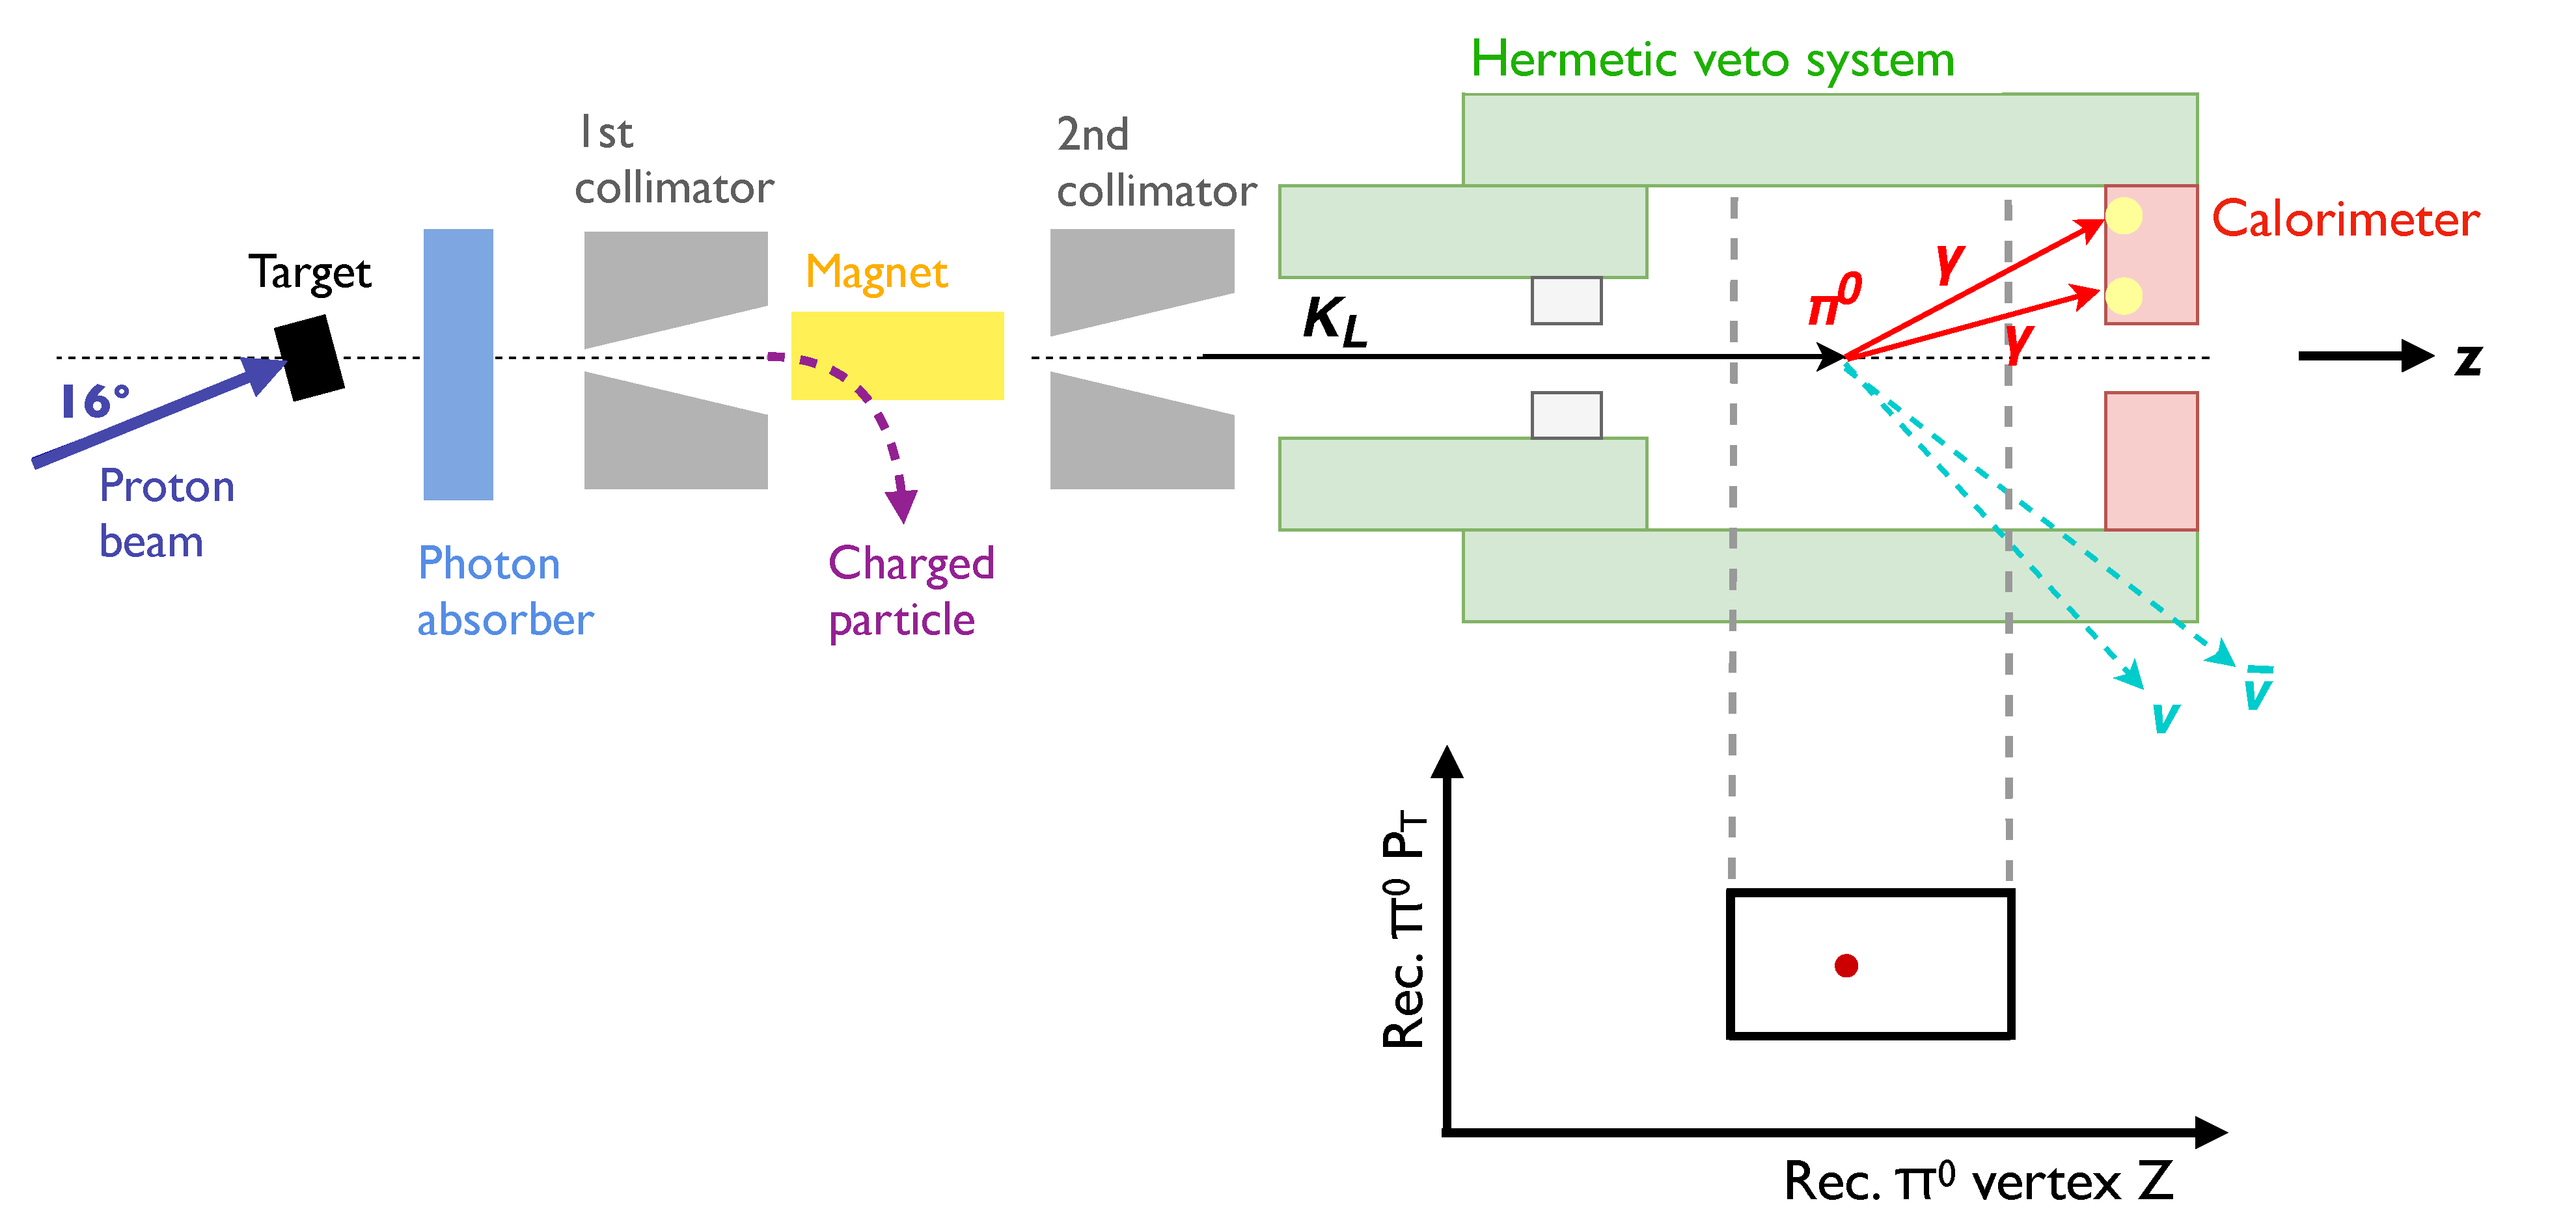
\includegraphics[width=0.99\textwidth]{Figures/Chapter3/schematic_ptz.pdf}
\caption{A schematic diagram of the search for $K_L^0 \to \pi^0 \nu \overline{\nu}$ at the KOTO experiment. }
\label{fig:schematic_KOTO}
\end{center}
\end{figure}

%%%%
% 3-1-1 signal identification

\subsection{Signal identification}

A reconstructable event requires exact two photons from a $\pi^0$ hitting the calorimeter, as shown in Figure \ref{fig:KOTO_signal_3D}. Based on four-momentum conservation, the opening angle ($\theta$) between two photons is calculated by %\mynobreakpar
%
\vspace{1em}
\begin{align}
\cos{\theta} = 1 - \frac{M_{\pi^0}^2}{2 E_1 E_2 },
\end{align}

\noindent 
where $E_1$ and $E_2$ are the two photon energies, and $M_\pi^0$ is the nominal $\pi^0$ mass. By assuming the $\pi^0$ decays at the center of the beam  (z-axis by convention), the $\pi^0$ vertex $Z$ ($Z_{vtx}$) can be obtained. Subsequently, the momenta of the two photons and the $\pi^0$ can be therefore calculated. Because neutrinos are invisible, the $\pi^0$ transverse momentum ($P_T$) is expected to be large.  

The signal box is defined on the reconstructed $(P_T - Z_{vtx})$ plane, as shown in the bottom part of Figure \ref{fig:schematic_KOTO}. Any event lies inside the signal box is treated as the "signal candidate". During the analysis, the side-band region is utilized to predict the distribution inside the signal region. Not until the data behavior is fully understood can the events in the signal region be accessed. This strategy, so-called "blind analysis", is adopted to dispel the prejudice against the signal candidates.

\begin{figure}[h]
\begin{center}
\captionsetup{width=.99\linewidth}
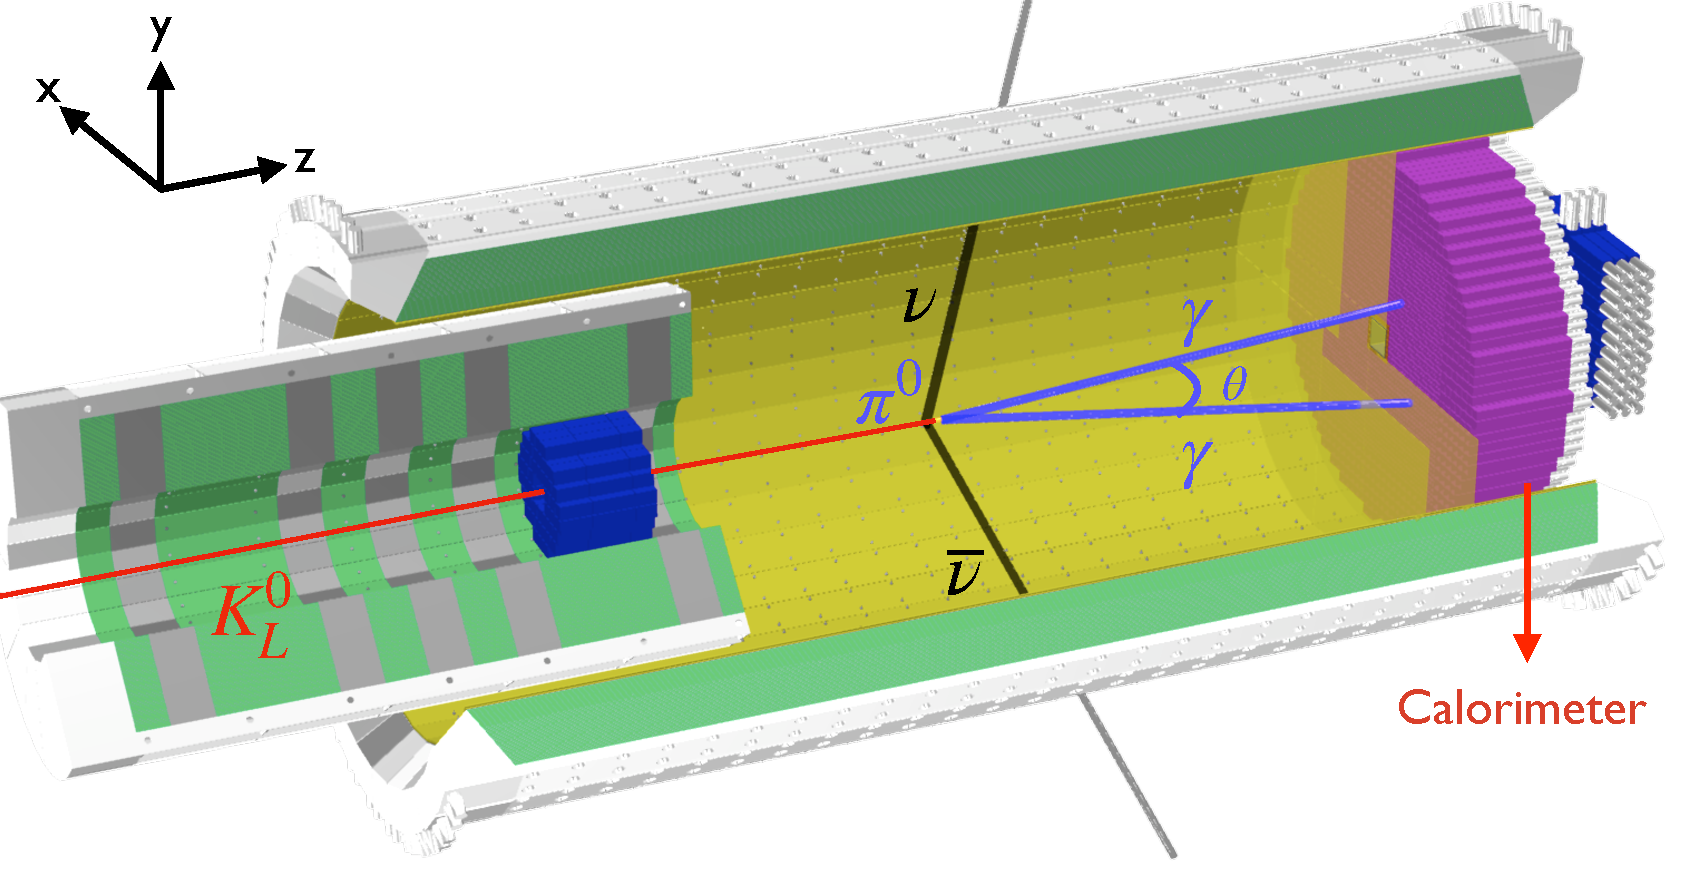
\includegraphics[width=0.8\textwidth]{Figures/Chapter3/Detector_3D.pdf}
\caption{A graphical illustration of a reconstructable ${K_L^0 \to \pi^0 \nu \overline{\nu}}$ decay inside the KOTO detector.}
\label{fig:KOTO_signal_3D}
\end{center}
\end{figure}

%%%
% 3-1-2 major background sources

\subsection{Major background sources}
Any source that can have two hits in the calorimeter potentially mimic signals. By considering the composition of the KOTO beam, the background is primarily induced by $K_L^0$s or neutrons.

\subsubsection{$K_L^0$-induced Background}
Table \ref{tab:KL_decay} lists the main $K_L^0$ decays. Because almost all of the $K_L^0$-decay channels are accompanied by charged particles or more than two photons, the detection of those particles is the most powerful and straightforward approach to suppressing the $K_L^0$ backgrounds. The inefficiency of the detector is essentially translated as the background level. The exception is the $K_L^0\to2\gamma$ decay, which is instead reduced by requiring large $P_T$. 

%In principle, all of them can have two hits in the calorimeter and thus mimic the signals. The suppression of the $K_L^0$-induced backgrounds typically relies on the following approaches: \mynobreakpar

%\begin{itemize}
%\item \textbf{Charge veto}. \\
%The $K_L^0$-decay channels accompanied by charged particles are suppressed by requiring the absence of charged particle hits in the veto system.

%\item \textbf{Photon veto.} \\
%The $K_L^0$-decay channels accompanied by extra photons are suppressed by requiring the absence of photon hits in the veto system.

%\item \textbf{Large $\pi^0$ $P_T$.} \\
%The $K_L^0\to2\gamma$ decay is suppressed by requiring large $P_T$ because there is no any missing particle.

%%%%%%%%%%%%%%%%%%%%%%%%%%%%%
%%% Branching ratio table %%%
%%%
%\end{itemize}

\begin{table} [h]
\centering
\caption{Main $K_L^0$ decays with their branching ratios \parencite{PDG18} . }
\label{tab:KL_decay}
%
\small
\begin{tabular}{l l}
\dtoprule
\rowcolor{LightCyan}
%\mc{1}{Decay mode} & \mc{1}{Branching ratio} \\
Decay mode & Branching ratio \\
\midrule[0.5pt]
$K_L^0 \rightarrow \pi^{\pm} e^{\mp} \nu_e$ ($K_{e3}^0$) & $(40.55 \pm 0.11) \%$ \\
$K_L^0 \rightarrow \pi^{\pm} \mu^{\mp} \nu_{\mu}$ ($K_{\mu 3}^0$) & $(27.04 \pm 0.07) \%$  \\
$K_L^0 \rightarrow 3 \pi^0$ & $(19.52 \pm 0.12) \%$ \\
$K_L^0 \rightarrow \pi^+ \pi^- \pi^0$ & $(12.54 \pm 0.05) \%$  \\
$K_L^0 \rightarrow \pi^{\pm} e^{\mp} \nu_e \gamma$ & $(3.79 \pm 0.06) \times 10^{-3}$ \\
$K_L^0 \rightarrow \pi^+ \pi^-$ & $(1.967 \pm 0.01) \times 10^{-3}$ \\
$K_L^0 \rightarrow \pi^0 \pi^0$ & $(8.64 \pm 0.06) \times 10^{-4}$ \\
$K_L^0 \rightarrow \pi^{\pm} \mu^{\mp} \nu_{\mu} \gamma$ & $(5.65 \pm 0.23) \times 10^{-4}$ \\
$K_L^0 \rightarrow 2 \gamma$ & $(5.47 \pm 0.04) \times 10^{-4}$ \\
\dbottomrule
\end{tabular}
%
\end{table}

%%%%%%%%%%%%%%%%%%

\subsubsection{Neutron-induced Background}

The neutrons from the periphery of the beam (halo neutrons) are also threats. If a neutron hits the detector material, a $\pi^0$ or a $\eta$ might be created through the neutron interactions and decays to two photons hitting the calorimeter. A halo neutron can also enter the calorimeter, two hits might be subsequently generated through the hadronic interactions. Their suppression typically relies on the kinematic variables and the shower shapes.

%----------------------------------------------------------------------------------------
%	SECTION 2: accelerator  
%----------------------------------------------------------------------------------------

\section{Accelerator}

The KOTO experiment is located at Hadron Experimental Facility (HEF) of Japan Proton Accelerator Research Complex (J-PARC) \parencite{JPARC_intro}. The proton beam travels along the orange line in Figure \ref{fig:JPARC_site} before striking the target. Protons are generated at the end of linear particle accelerator (LINAC) \parencite{LINAC}, injected to 3-GeV rapid cycling synchrotron \parencite{RCS},  then accelerated to 30~GeV at main ring synchrotron \parencite{MR}, and eventually delivered to HEF.

\begin{figure}[h]
\begin{center}
\captionsetup{width=.99\linewidth}
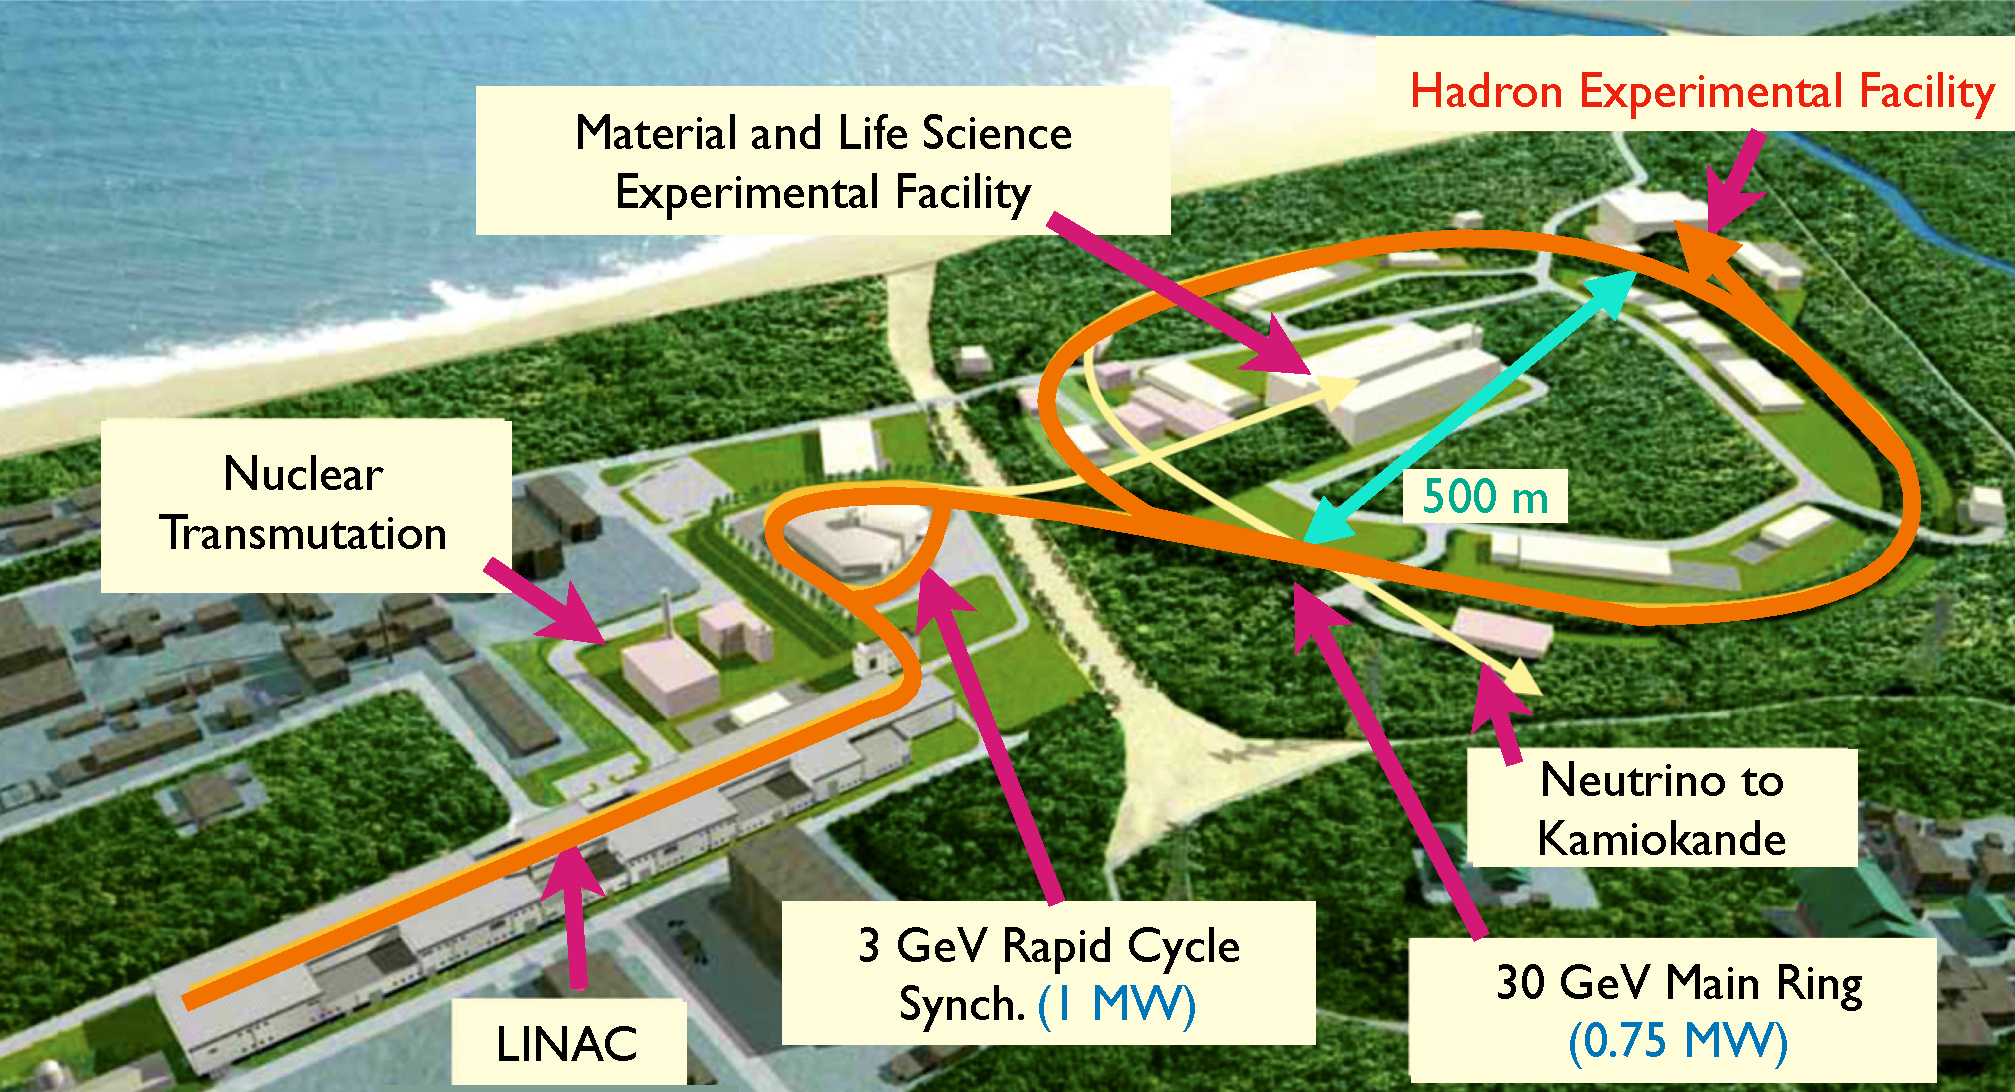
\includegraphics[width=0.75\textwidth]{Figures/Chapter3/JPARC_facility.pdf}
\caption{Entire view of J-PARC (Figure courtesy of \parencite{JPARC_intro} with modifications). The orange line indicates the path of the proton beam.}
\label{fig:JPARC_site}
\end{center}
\end{figure}
 
The proton beam for KOTO is slowly extracted for 2~s and repeated every "spill" of 5.2~s\footnote{The spill length was xxx sec in xxxx and gradually decreased to xxx sec in xxxx.}. Notably, the beam intensity $I=I(t)$ varies with time and the distribution of $I(t)$ is known as the beam structure. The spiky beam structure is not desirable because the instantaneous rate causes the pileup of events, which introduces the signal loss. In order to characterize the beam structure, the flatness level is qualified by the duty factor \parencite{MR}: \mynobreakpar
%
%\vspace{1em}
\begin{align}
\textit{Duty} = \dfrac{\left( \int_{T_1}^{T_2} I(t) dt  \right)^2}{\int_{T_1}^{T_2} dt \int_{T_1}^{T_2} I(t)^2 dt},
\end{align}

\noindent
where $T_1$ and $T_2$ are the times determining the gate width. The duty factor is 100\% if the beam structure is perfectly flat. During the beam operation from 2016 through 2020, the measured duty factor is about 60\%.

%----------------------------------------------------------------------------------------
%	SECTION 3: Detector
%----------------------------------------------------------------------------------------
\section{Detector}

As discussed in Section \ref{sec:basic}, the suppression of $K_L^0$-induced backgrounds strongly relies on the extensive detection of the charged particles and extra photons. The KOTO detector features in the hermetic veto system and the low inefficiency against those particles. Double decay chambers are adopted to identify whether an event is caused by an upstream $K_L^0$ decay. 

Figure \ref{fig:detector} shows an overview of the KOTO detector with the conventional coordinate system. The features of each subdetector are explained as follows.% and summarized in Table~\ref{tab:detector}.
 
%%%
% KOTO detector figure 
%%%
\begin{sidewaysfigure}
\centering
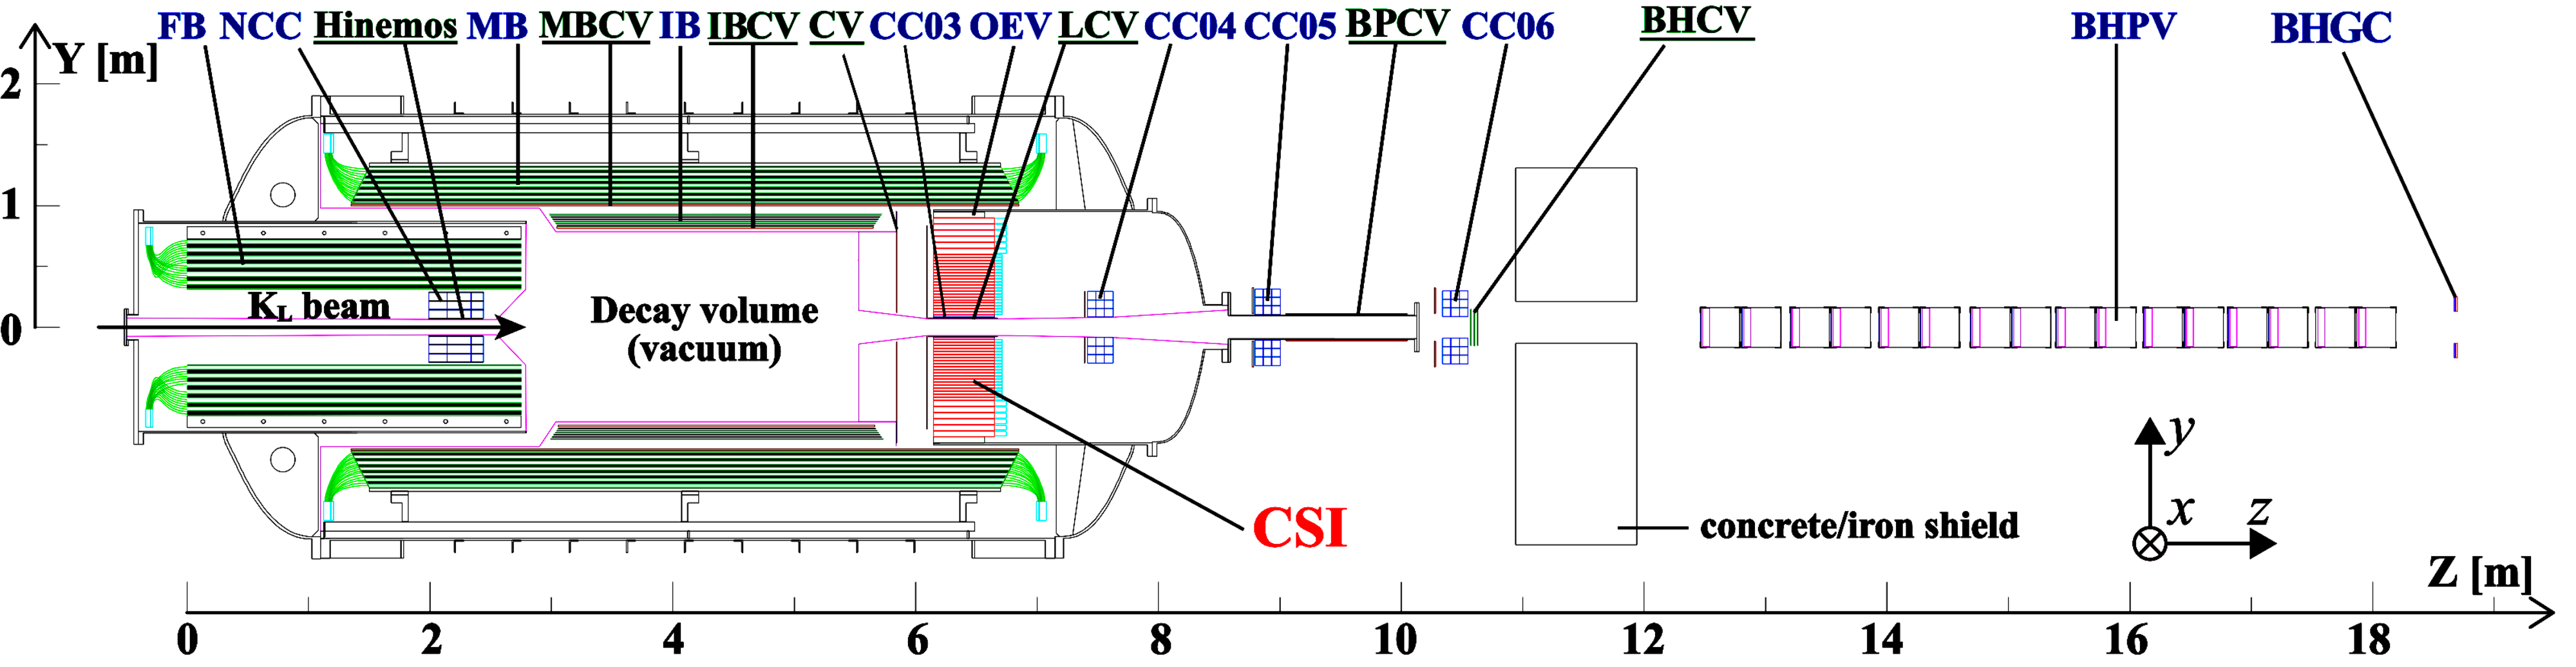
\includegraphics[width=0.99\textwidth]{Figures/Chapter3/KOTODetector2018.pdf}
\caption{Overview of the KOTO Detector. Each subdetector labeled with its abbreviated name in blue (green) is the photon (charged particle) veto counter. The conventional coordinate system of KOTO is displayed.}
\label{fig:detector}
\end{sidewaysfigure}

%%%%%%%%%%%%%%%%%%%%%%%
% KOTO Detector TABLE %
%%%%%%%%%%%%%%%%%%%%%%%
%
%\begin{table}[h]
%\centering
%\begin{small}
%\caption{Summary of the KOTO detector.}
%\label{tab:detector}

%\begin{tabular}{b c c c c}
%\dtoprule
%\rowcolor{LightCyan}
%\mc{1}{Detector} & \mc{1}{Type} & \mc{1}{Purpose} & \mc{1}{Configuration} & \mc{1}{Performance}
% \\
%\midrule[0.5pt]
%CSI  & \makecell{CsI crystals} & \makecell{Photon \\ measurement} & \makecell{Endcap: $z = \SI{6168}{mm}$ \\ Depth: $l = \SI{50}{mm}$ \\ Diameter: $d=\SI{1.9}{m}$ } & \makecell{good} \\ \hline 
%CV   & Plastic scintillator & Charged particle veto & \makecell{Endcap: $z = \SI{6168}{mm}$ \\ Depth: $l = \SI{50}{mm}$ \\ Diameter: $d=\SI{1.9}{m}$ } & good \\ \hline
%NCC  & 3 CsI crystals & suppression & \makecell{Endcap: $z = \SI{6168}{mm}$ \\ Depth: $l = \SI{50}{mm}$ \\ Diameter: $d=\SI{1.9}{m}$ } & good \\ \hline
%Hinemos  & 3 CsI crystals & suppression & \makecell{Endcap: $z = \SI{6168}{mm}$ \\ Depth: $l = \SI{50}{mm}$ \\ Diameter: $d=\SI{1.9}{m}$ } & good \\ \hline
%FBAR & \makecell{Lead-scintillator \\ sandwich} & Photon veto & \makecell{Endcap: $z = \SI{6168}{mm}$ \\ Depth: $l = \SI{50}{mm}$ \\ Diameter: $d=\SI{1.9}{m}$ } & good \\ \hline
%CBAR &  \makecell{Lead-scintillator \\ sandwich} & Photon veto & \makecell{Endcap: $z = \SI{6168}{mm}$ \\ Depth: $l = \SI{50}{mm}$ \\ Diameter: $d=\SI{1.9}{m}$ } & good \\ \hline
%IB   &  \makecell{Lead-scintillator \\ sandwich} & Photon veto & \makecell{Endcap: $z = \SI{6168}{mm}$ \\ Depth: $l = \SI{50}{mm}$ \\ Diameter: $d=\SI{1.9}{m}$ } & good \\ \hline
%MBCV & Plastic Scintillator & Charged particle veto & \makecell{Endcap: $z = \SI{6168}{mm}$ \\ Depth: $l = \SI{50}{mm}$ \\ Diameter: $d=\SI{1.9}{m}$ } & good \\ \hline
%IBCV & Plastic scintillator & Charged particle veto & \makecell{Endcap: $z = \SI{6168}{mm}$ \\ Depth: $l = \SI{50}{mm}$ \\ Diameter: $d=\SI{1.9}{m}$ } & good \\ \hline
%OEV  & test & Photon measurement & \makecell{Endcap: $z = \SI{6168}{mm}$ \\ Depth: $l = \SI{50}{mm}$ \\ Diameter: $d=\SI{1.9}{m}$ } & good \\ \hline
%CC03 & CsI crystals & Photon measurement & \makecell{Endcap: $z = \SI{6168}{mm}$ \\ Depth: $l = \SI{50}{mm}$ \\ Diameter: $d=\SI{1.9}{m}$ } & good \\ \hline
%LCV  & Plastic scintillator & Charged particle veto & \makecell{Endcap: $z = \SI{6168}{mm}$ \\ Depth: $l = \SI{50}{mm}$ \\ Diameter: $d=\SI{1.9}{m}$ } & good \\ \hline
%CC04 & \makecell{CsI crystals \\ Plastic scintillators} & \makecell{photon veto \\ Charged particle veto} & test & good \\ \hline
%CC05 & \makecell{CsI crystals \\ Plastic scintillators} & \makecell{photon veto \\ Charged particle veto} & test & good \\ \hline
%CC06 & \makecell{CsI crystals \\ Plastic scintillators} & \makecell{photon veto \\ Charged particle veto} & test & good \\ \hline
%BPCV & Plastic Scintillator & measurement & \makecell{Endcap: $z = \SI{6168}{mm}$ \\ Depth: $l = \SI{50}{mm}$ \\ Diameter: $d=\SI{1.9}{m}$ } & good \\ \hline
%BHCV & Wire chamber & Photon measurement & \makecell{Endcap: $z = \SI{6168}{mm}$ \\ Depth: $l = \SI{50}{mm}$ \\ Diameter: $d=\SI{1.9}{m}$ } & good \\ \hline
%BHPV & test & Photon measurement &  \makecell{Endcap: $z = \SI{6168}{mm}$ \\ Depth: $l = \SI{50}{mm}$ \\ Diameter: $d=\SI{1.9}{m}$ } & good \\ \hline
%BHGC & \v{C}erenkov counter & Photon veto & \makecell{Endcap: $z = \SI{6168}{mm}$ \\ Depth: $l = \SI{50}{mm}$ \\ Diameter: $d=\SI{1.9}{m}$ } & good \\
%\dbottomrule
%\end{tabular}
%\end{small}
%\end{table}

%%
%% 3-1 vacuum
%%%%%%%%%%%%%%%
\subsection{Vacuum System}
Vacuum is an essential condition to reduce the $\pi^0$ production through the neutron interactions with gas. The high vacuum environment is required to neglect the gas background but introduce the outgassing from the detector material. Consequently, the "membrane" (pink line in Figure~\ref{fig:detector}), which is a thin (0.2~mm) and loss-mass material to eliminate the interactions with particles, is installed to separate the decay region from the detector space. The decay volume is highly evacuated at 5~$\times$~10$^{-5}$~Pa and the rest is maintained at 1~Pa as a buffer. 

%%
%% 3-2 CSI
%%%%%%%%%%%%%%%%%%

\subsection{Electromagnetic Calorimeter}
The electromagnetic calorimeter, which is comprised of 2716 undoped cesium iodide crystals, is primarily utilized to measure the positions and energies of photons for the $\pi^0$ reconstruction \parencite{CSI}. The nickname "CSI" is given according to the material. As Figure~\ref{fig:CSI_config} shows, the 2240 small crystals have a size of 2.5~$\times$~2.5~$\times$~50~cm$^3$ arranged in the inner region, and the 476 large ones have a size of 5.0~$\times$~5.0~$\times$~50~cm$^3$ arranged in the outer region. The depth is corresponding to 27 radiation lengths ($X_0$), which suggests the negligible inefficiency of photon due to punch-through. A square hole is left in the center to keep the calorimeter in a relatively quieter environment. 

\begin{figure}[h]
\begin{center}
\captionsetup{width=.99\linewidth}
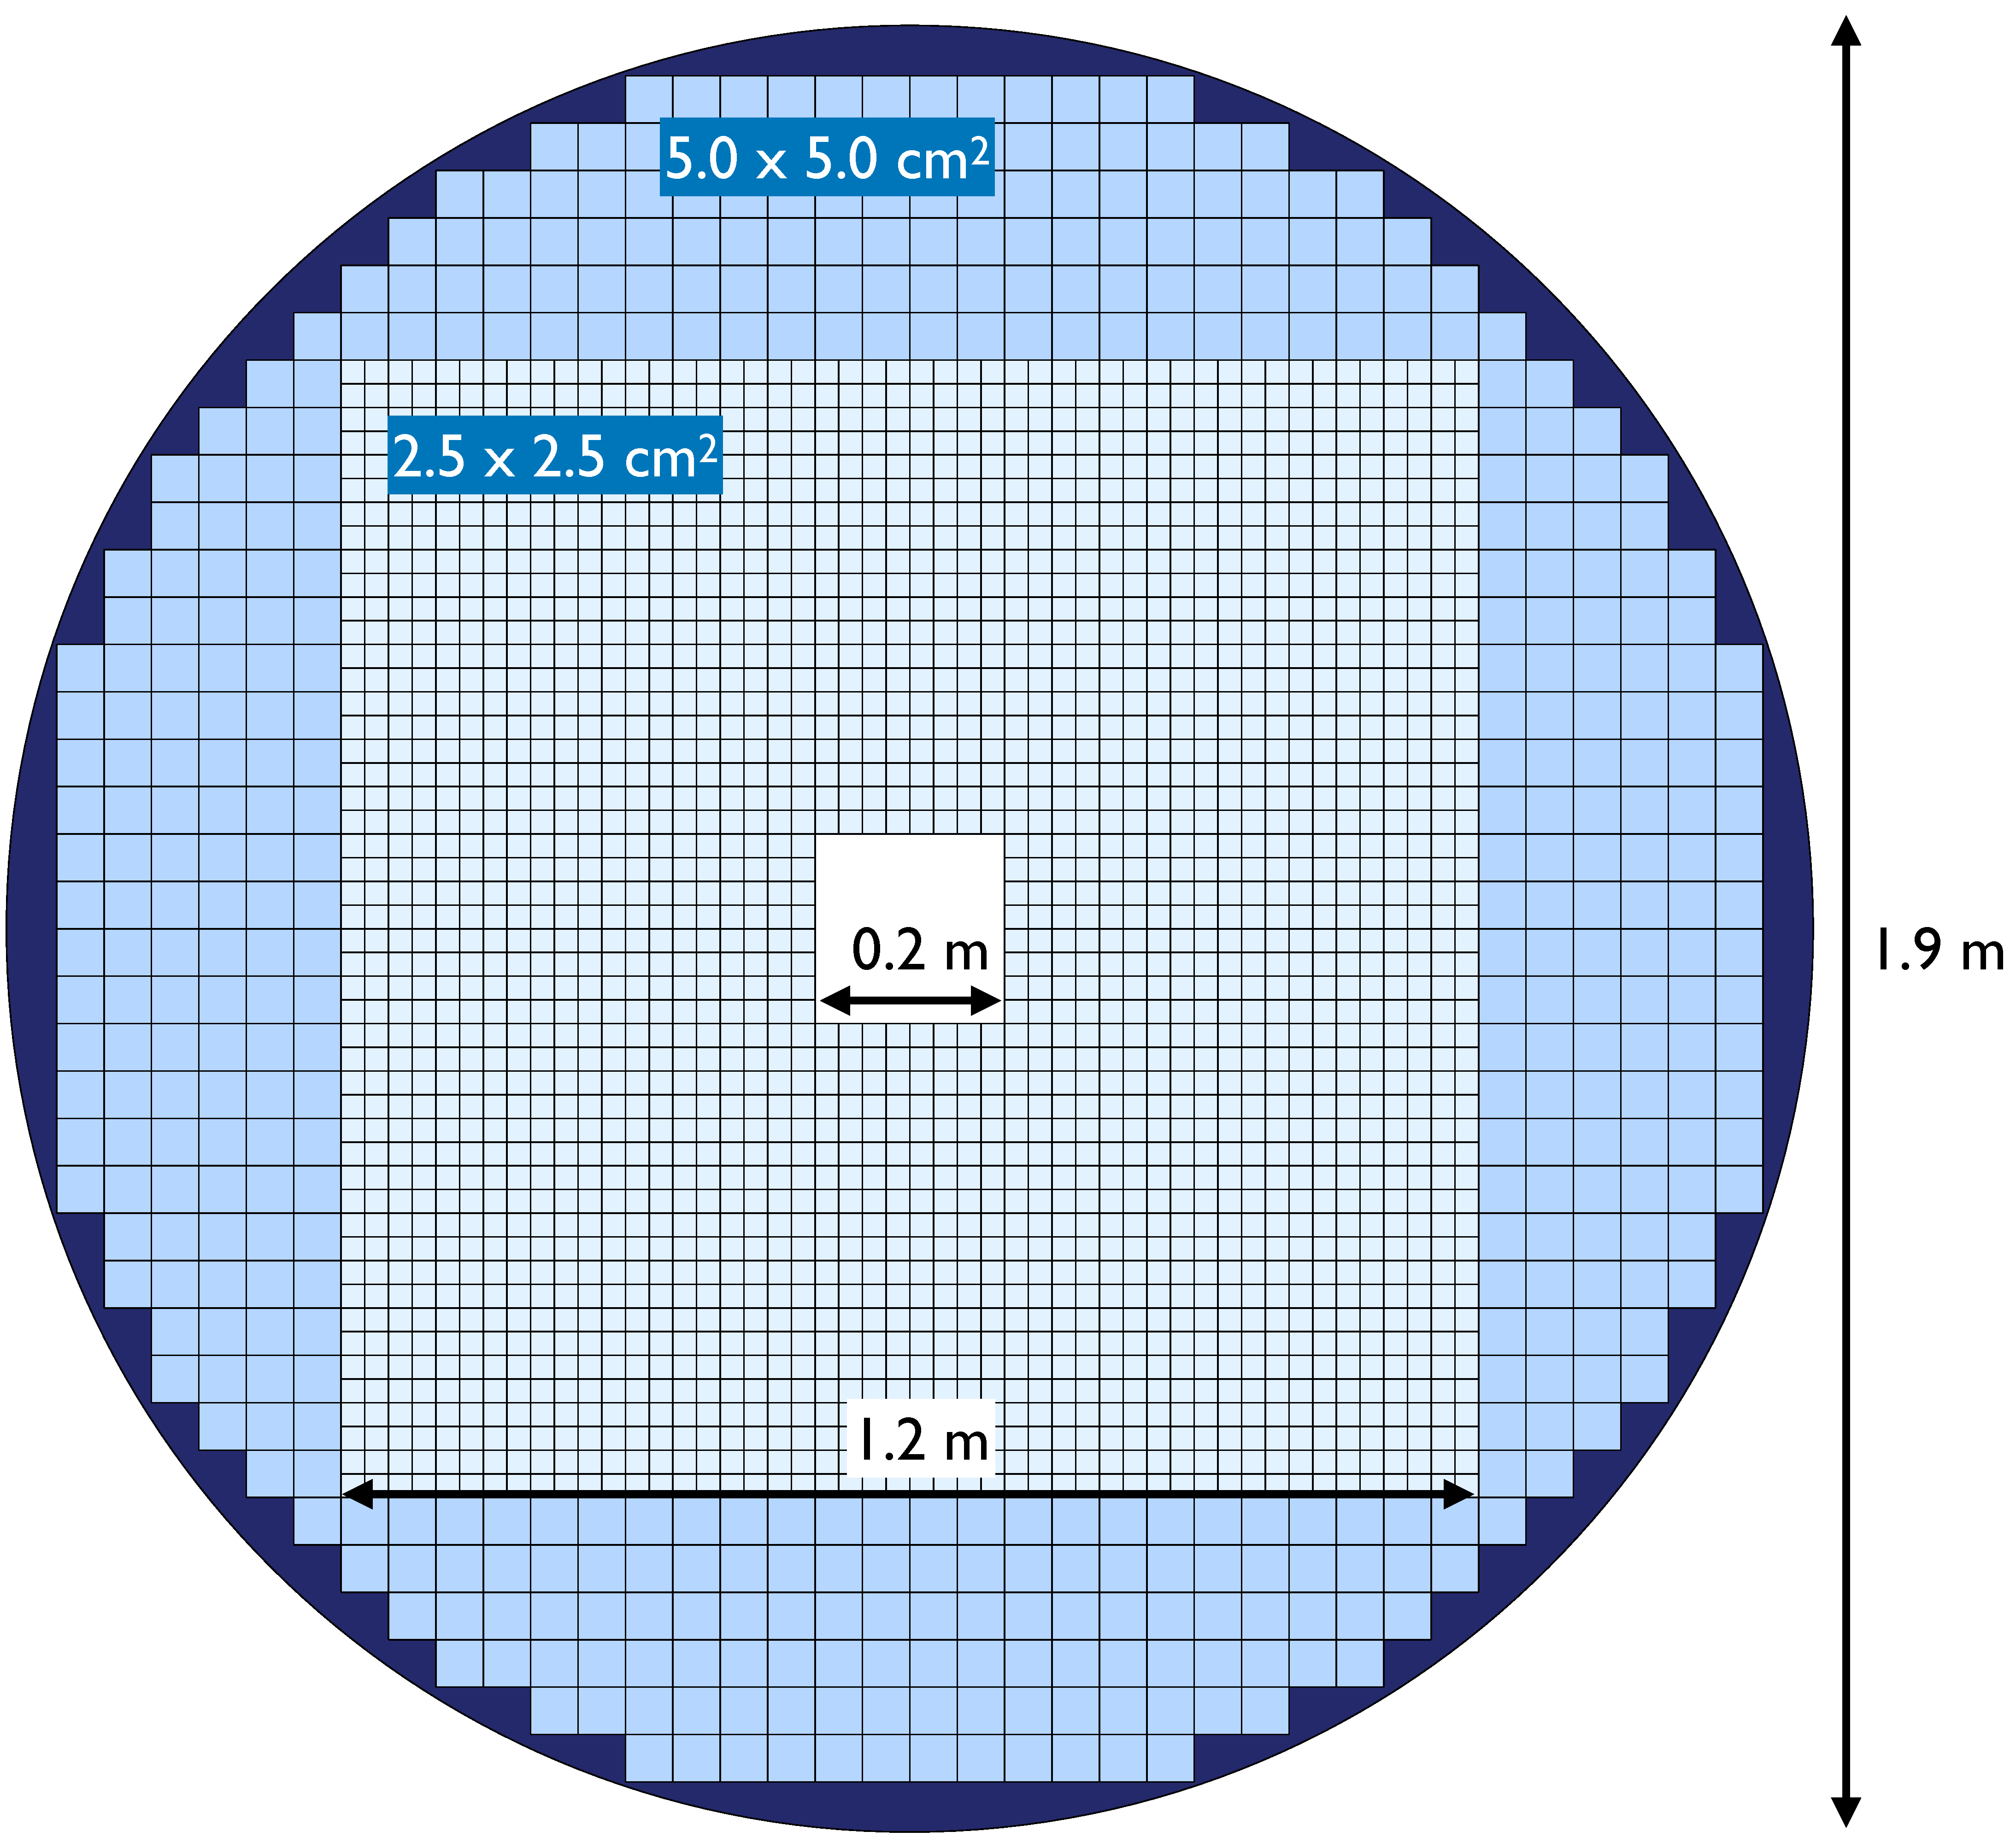
\includegraphics[width=0.6\textwidth]{Figures/Chapter3/CSI_config.pdf}
\caption{An upstream view of the CsI calorimeter \parencite{CSI}.}
\label{fig:CSI_config}
\end{center}
\end{figure}

When a photon hits the calorimeter, the electromagnetic shower is induced and the energy hence spreads out across the adjacent crystals as a cluster. A photomultiplier tube (PMT) is contacted with each crystal for collecting the scintillation lights inside\footnote{A silicone cookie for optical contact \parencite{CSI_cookie} and a UV filter for elimiating the slow components in scintillation lights are inserted between the crystal and the PMT.}. The energy deposit can be obtained by the amount of photo-electrons emitted from the PMT because of the proportionality between two quantities. Moreover, the typical cluster size is characterized by the Mol\`{e}re radius of 3.57~cm \parencite{PDG18}, which is longer than the width of the small crystals. This feature benefits the position resolution and the discrimination power against the shower overlaps.

The performance of the calorimeter is evaluated; for the inner region, the energy resolution is
%
%\vspace{1em}
\begin{align}
\sigma_E / E = \left( 0.66 \oplus 1.81 /\sqrt{E~\text{[GeV]}} \right)~\%, 
\end{align}

\noindent
where $E$ is the total energy and $\oplus$ stands for the quadratic sum, and the position resolution is
%
%\vspace{1em}
\begin{align}
\sigma_{pos} = \left( 1.99 \oplus 3.95 /\sqrt{E~\text{[GeV]}} \right)~\text{mm}.
\end{align}


 
%% 
%% 3-3 CV
%%%%%%%%%%%%%%%%

\subsection{Charge Veto Counter}
If two charged particles in the ${K_L^0 \to \pi^{\pm} e^{\mp} \nu}$ decay hit the calorimeter, two clusters can be generated and misidentified as a $\pi^0$ decay. The Charged Veto counter (CV) \parencite{CV} implemented near the surface of the calorimeter is therefore critical for the detection of the electric charge. Because the ${\mathcal{BR}(K_L^0 \to \pi^{\pm} e^{\mp} \nu)}$ is $\mathcal{O}(1)$, CV is demanded to have a high detection efficiency to charged particles to reduce the ${K_L^0 \to \pi^{\pm} e^{\mp} \nu}$ background by a factor of $\mathcal{O}(10^{11})$. The minimal interaction with hadrons is also essential to avoid introducing extra backgrounds; a halo neutron hits the material and generates $\pi^0$ or $\eta$ that decays to two photons. This suggests the low-mass material for eliminating the $\pi^0$ or $\eta$ productions. 

CV has two layers 251~mm apart. As Figure \ref{fig:CV_config} shows, the upstream (downstream) CV layer has 44 (48) plastic-scintillator strips arranged in four quadrants with a square hole at the center and each strip is attached with wavelength-shifting (WLS) fibers. The orientations of the strips in one layer are arranged perpendicularly to those in the other layer for locating the passage of a charged particle. These materials are sustained by a 0.8-mm-thick carbon fiber reinforced plastic (CFRP) plate.

\begin{figure}[h]
\begin{center}
\captionsetup{width=.99\linewidth}
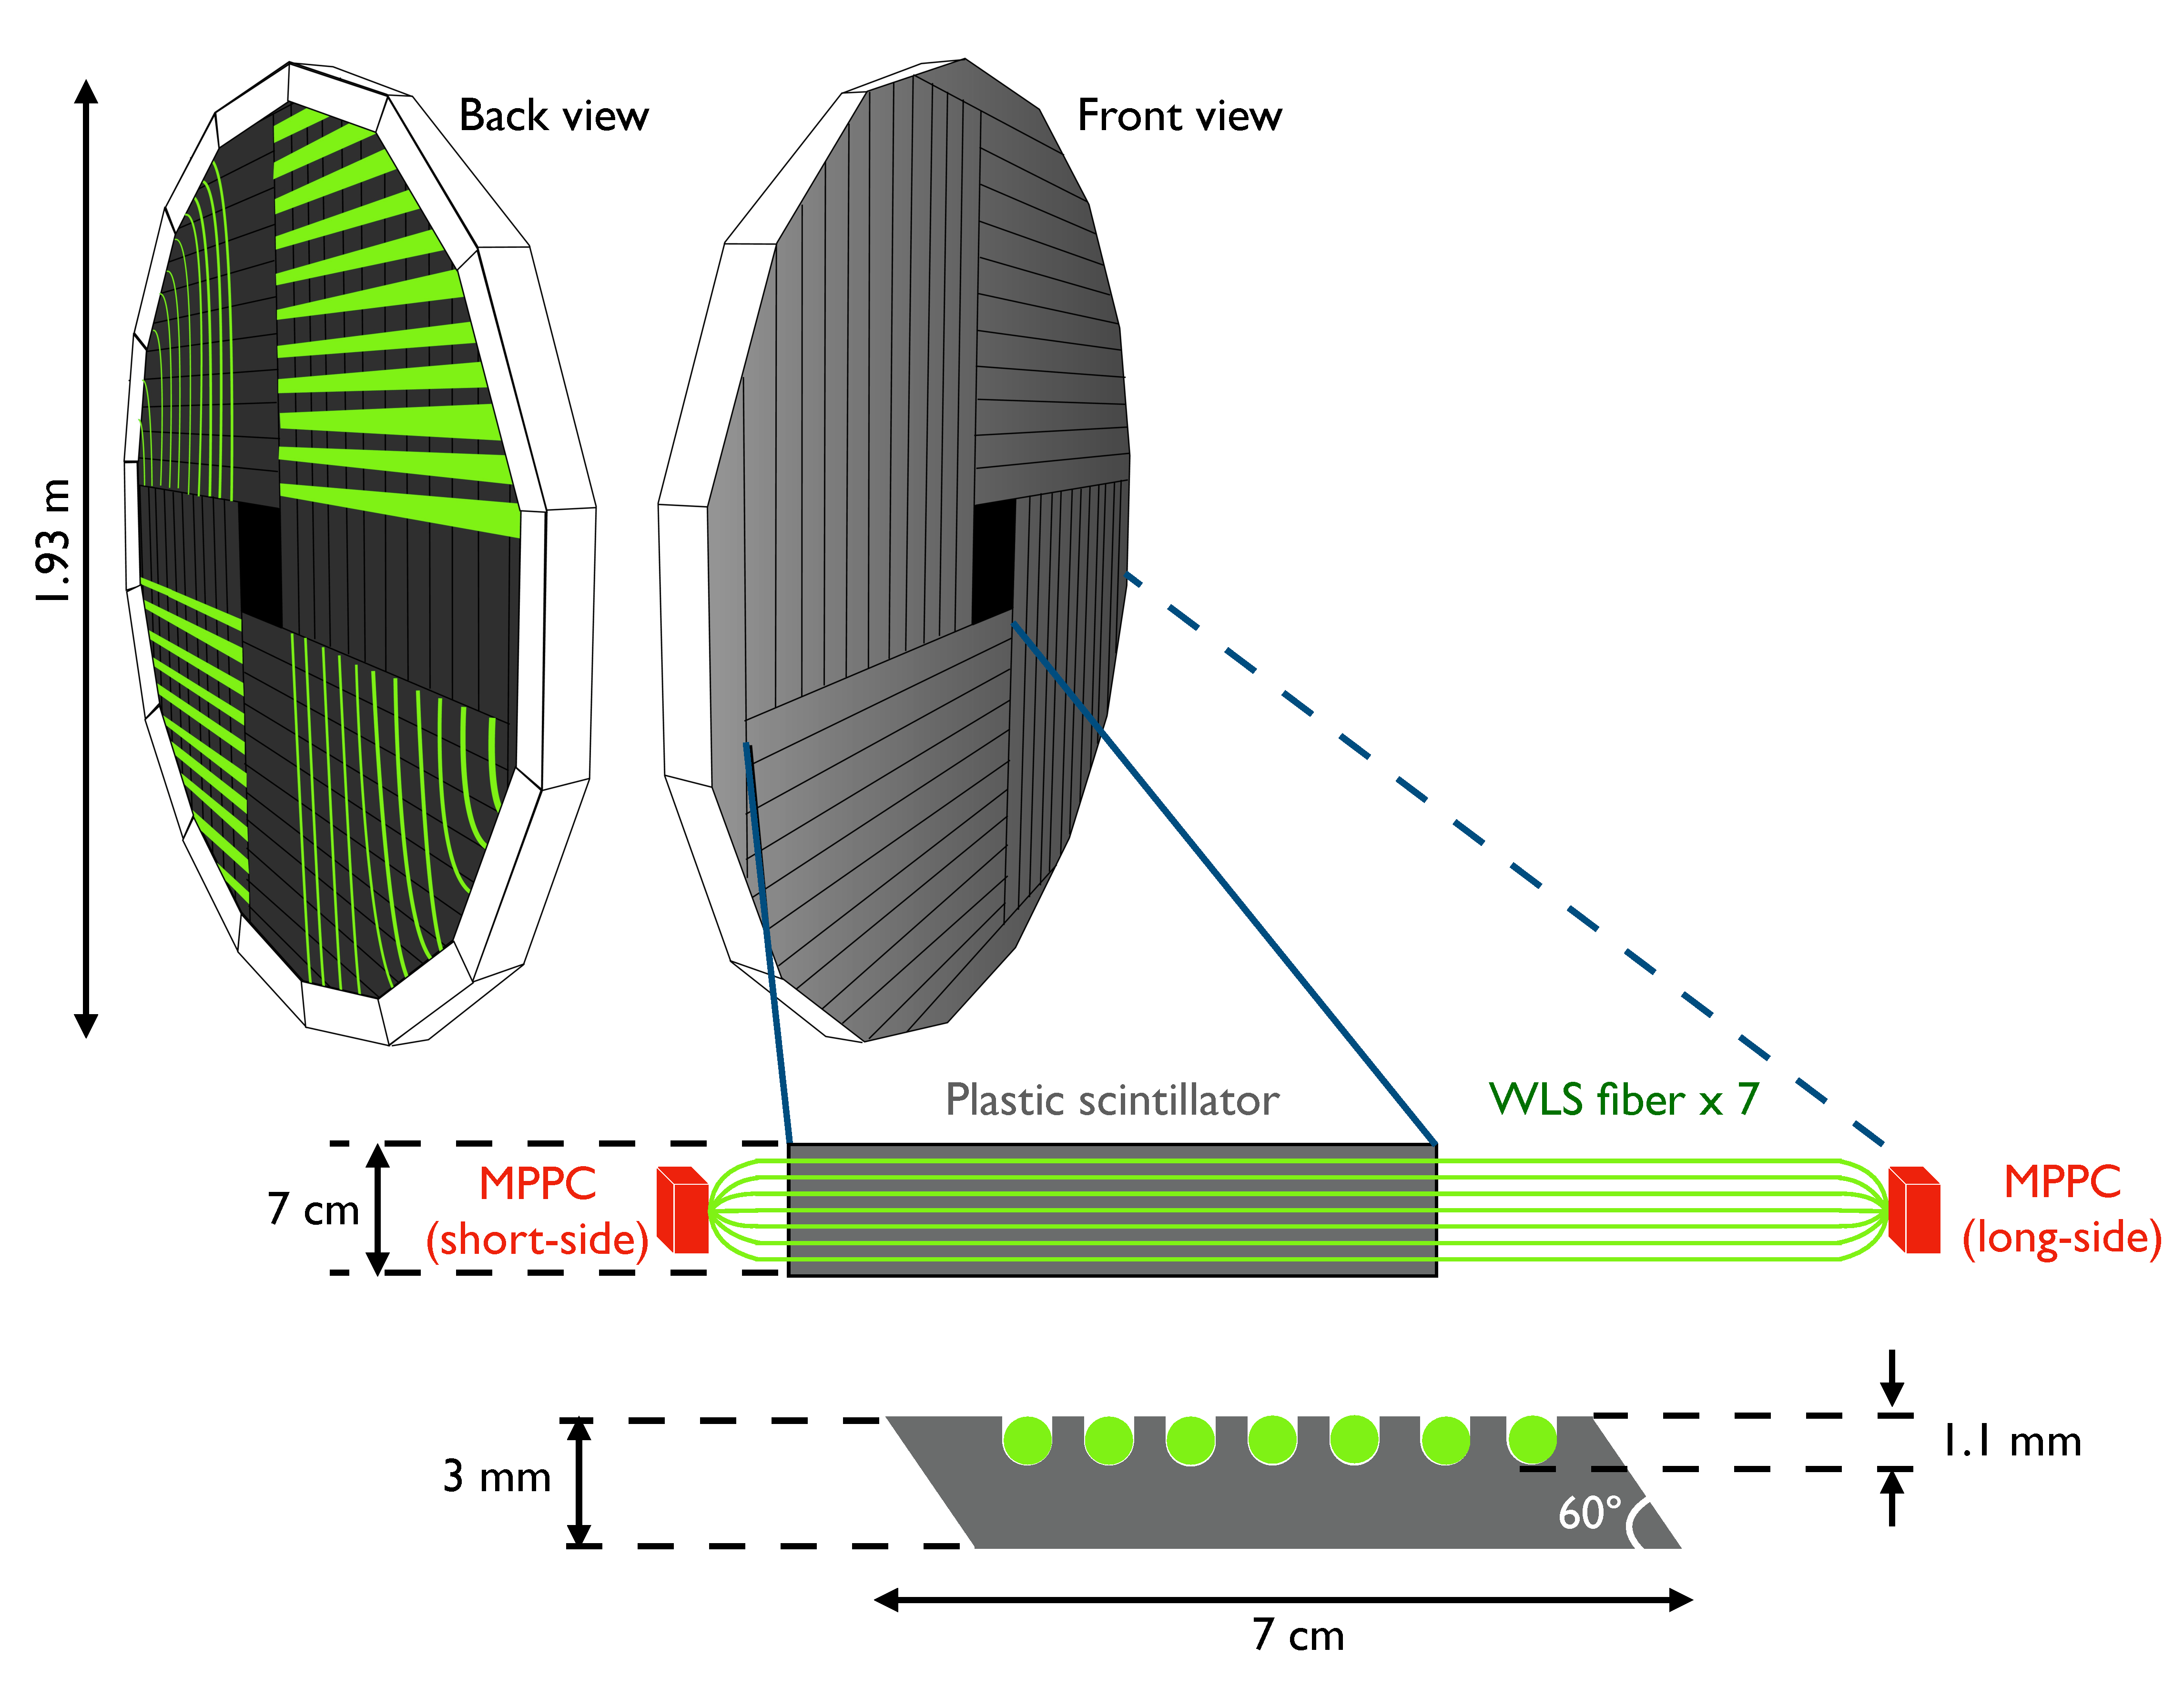
\includegraphics[width=0.99\textwidth]{Figures/Chapter3/CV_config.pdf}
\caption{A schematic diagram of a CV layer \parencite{CV, Maeda}.}
\label{fig:CV_config}
\end{center}
\end{figure}

The energy lost by a charged particle across the medium can yield the scintillation lights through the excitation and deexcitation of an atom. Those lights are guided by fibers and directed to multi-pixel photon counters (MPPC) at both ends. The photo-electrons emitted from MPPC form the pulses, which are used for veto analysis.

By considering the probability of missing two charged particles in both CV layers, the goal of the inefficiency per single layer is $<$ 10$^{-3}$, and the measured value is 1.5~$\times$~10$^{-5}$, which does satisfy the requirement.



%%
%% 3-4 Barrel veto counters
%%%%%%%%%%%%%%%%%%%%%%%%%%%%

\subsection{Barrel Veto Counters}
The ${K_L^0\to\pi^0\pi^0}$ background is considered to be one of the most challenging background sources at KOTO because its reduction principally depends on the detection efficiency to the two additional photons. Because the ${\mathcal{BR}(K_L^0\to\pi^0\pi^0)}$ is $\mathcal{O}(10^{-3})$, the overall photon inefficiency requires to be $<$ 10$^{-4}$ against 100-MeV photons.

The barrel veto counters cylindrically envelop the two decay chambers for detecting additional particles in $K_L^0$ decays: the Front Barrel counter (FB) for the upstream $K_L^0$ decays and the Main Barrel counter (MB) for the fiducial $K_L^0$ decays \parencite{barrel_veto}. Both FB and MB have been initially operated since the first data-taking in 2013. The Inner Barrel counter (IB)  \parencite{IB} was then installed inside MB to improve the detection capability in 2016. Due to the huge coverage, the performance of the barrel system is the leading factor to suppress the ${K_L^0\to\pi^0\pi^0}$ background.

As Figure \ref{fig:barrel_config} shows, FB, MB, and IB are composed of lead-scintillator sandwich and primarily responsible for photon veto. Lead is the dense material selected for the maximal absorption of photons. The lights are emitted by the neighboring scintillators and guided to PMTs by WLS fibers. At the innermost surface of IB and MB, the Inner Barrel Charged Veto counter (IBCV) and the Main Barrel Charged Veto counter (MBCV), which are composed of 10-mm-thick plastic scintillators with WLS fibers, are equipped for the charged particle detection respectively. IBCV covers the inner surface of IB completely while MBCV covers the counterpart of MB in the downstream region of IB. Both avoid the charged particles being absorbed quietly by the material exposed to the decay volume. 

%%% 
\begin{figure}[h]
\begin{center}
\captionsetup{width=.99\linewidth}
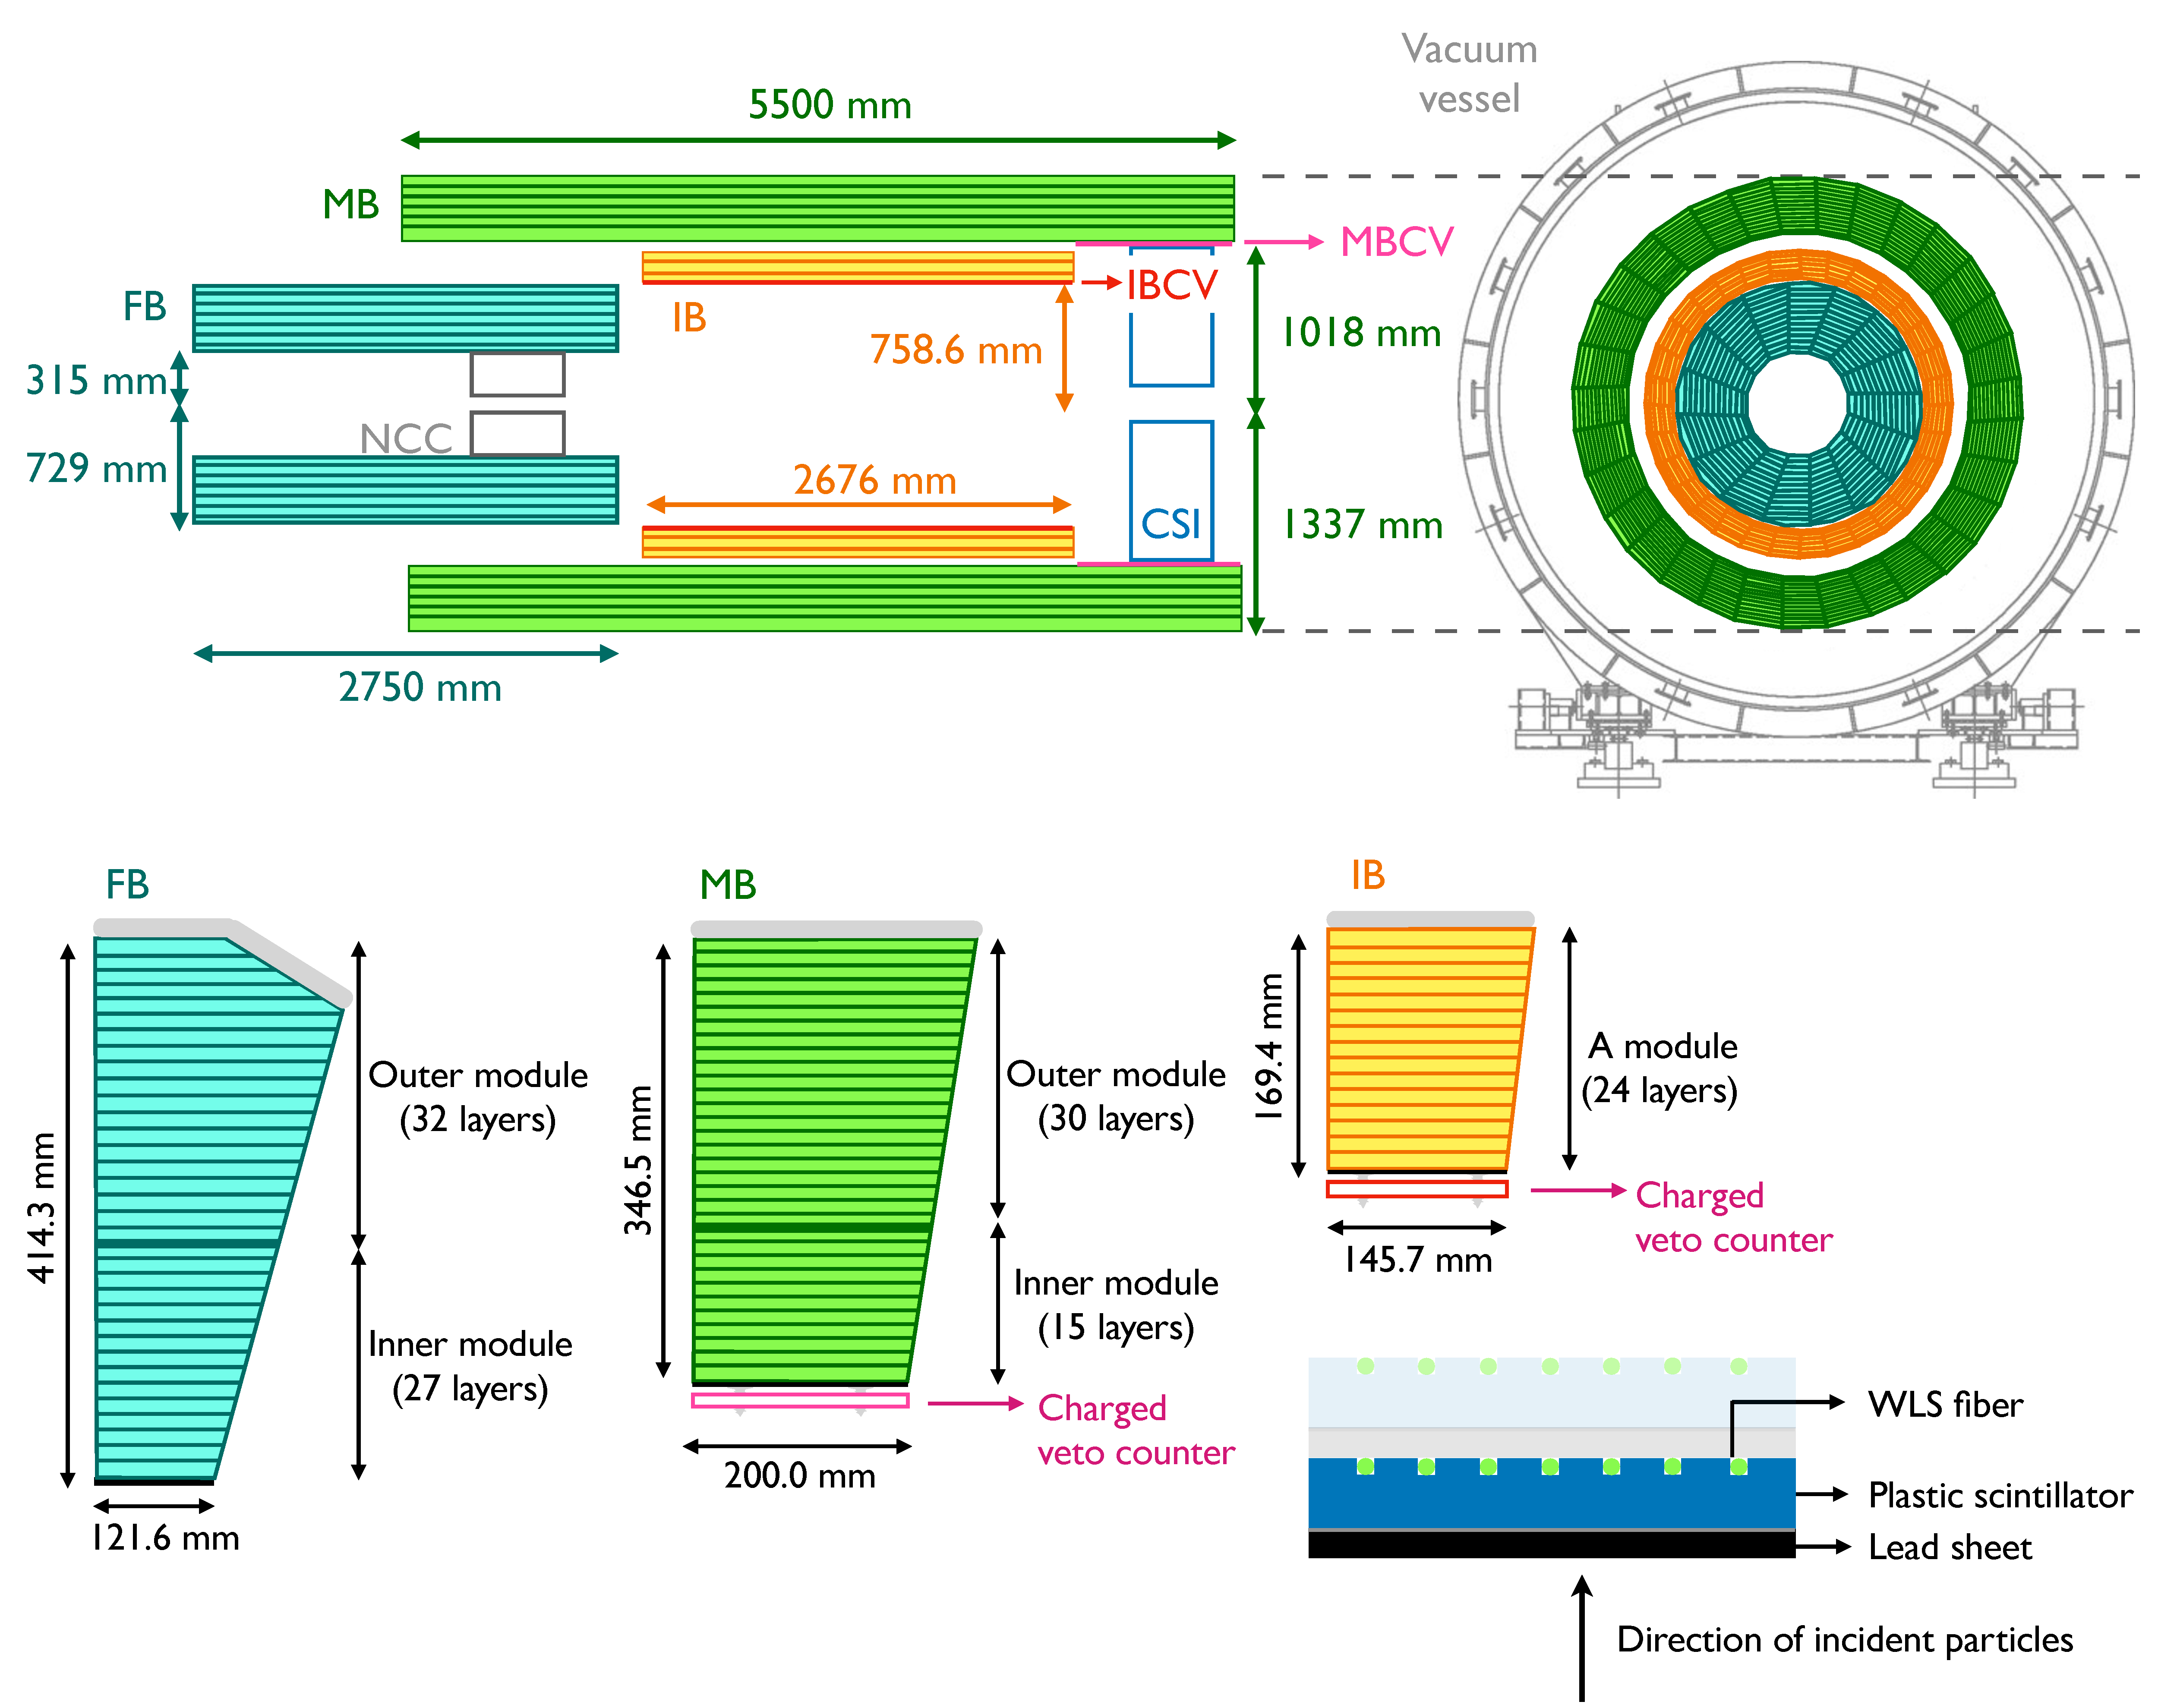
\includegraphics[width=0.99\textwidth]{Figures/Chapter3/Barrel_veto.pdf}
\caption{A schematic diagram of barrel veto counters \parencite{KOTO_intro, barrel_veto, IB}.}
\label{fig:barrel_config}
\end{center}
\end{figure}

The module arrangements and the readout units are summarized in Table~\ref{tab:barrel_property}. Those parameters determine the resolution of a photon hit in barrel veto system: the azimuthal direction by the number of modules, the depth of a photon conversion by the radial segmentation, and the longitudinal direction by the both-end readout. These variables render the background properties analyzable.

%%% barrel parameters %%%
\begin{table}[h]
\centering
\caption{Parameters of the barrel veto counters. }
\label{tab:barrel_property}
%
\small
\begin{tabular}{l c c c}
\dtoprule
\rowcolor{LightCyan}
Subdetector &  Thickness & Module arrangement &  Readout unit\\
\midrule[0.5pt]
FB & 16.5 $X_0$ & \makecell{16 inner modules \\ 16 outer modules} \vspace{0.5em} & \makecell{ Single-end readout \\ 32~$\times$~1~$=$~32~PMTs} \vspace{0.5em} \\
MB & 14.0 $X_0$ & \makecell{32 inner modules \\ 32 outer modules} & \makecell{ Both-end readout \\ 64~$\times$~2~$=$~128 PMTs}  \vspace{0.5em} \\
IB & 5.0 $X_0$ & \makecell{32 modules} & \makecell{ Both-end readout \\ 32~$\times$~2~$=$~64 PMTs } \vspace{0.5em} \\
IBCV & 10~mm & \makecell{32 modules} & \makecell{ Both-end readout \\ 32~$\times$~2~$=$~64~PMTs } \vspace{0.5em} \\
MBCV & 10~mm &  \makecell{16 modules} & \makecell{ Single-end readout \\ 16~$\times$~1~$=$~16~PMTs }\vspace{0.5em} \\
\dbottomrule
\end{tabular}
%
\end{table}

%%
%% 3-5 Neutron collar counter 
%%%%%%%%%%%%%%%%%%%%%%

\subsection{Neutron Collar Counter}
The Neutron Collar Counter (NCC) \parencite{NCC, NCC2} is placed inside the downstream end of FBAR and surrounds the $K_L^0$ beam as an upstream guard of the decay volume. Together with FBAR, the upstream ${K_L^0\to3\pi^0}$ and $K_L^0\to\pi^0\pi^0$ decays can be highly-suppressed. However, as its name hints, halo neutrons can interact with NCC and produce $\pi^0$s decaying to two photons as another background source. If the two photons or other secondary particles in the $\pi^0$ production can be detected in NCC itself, the neutron background is reducible.
 
This is realized by updoped cesium iodide crystals segmented into three parts along the beam direction, as shown in Figure~\ref{fig:NCC_config}. The 4.5~m-long crystals capture the activities inside and transmitted through WLS fibers. Furthermore, The individual readout provides the depth information, which is potentially a variable for the discrimination between photons and neutrons.

\begin{figure}[h]
\begin{center}
\captionsetup{width=.99\linewidth}
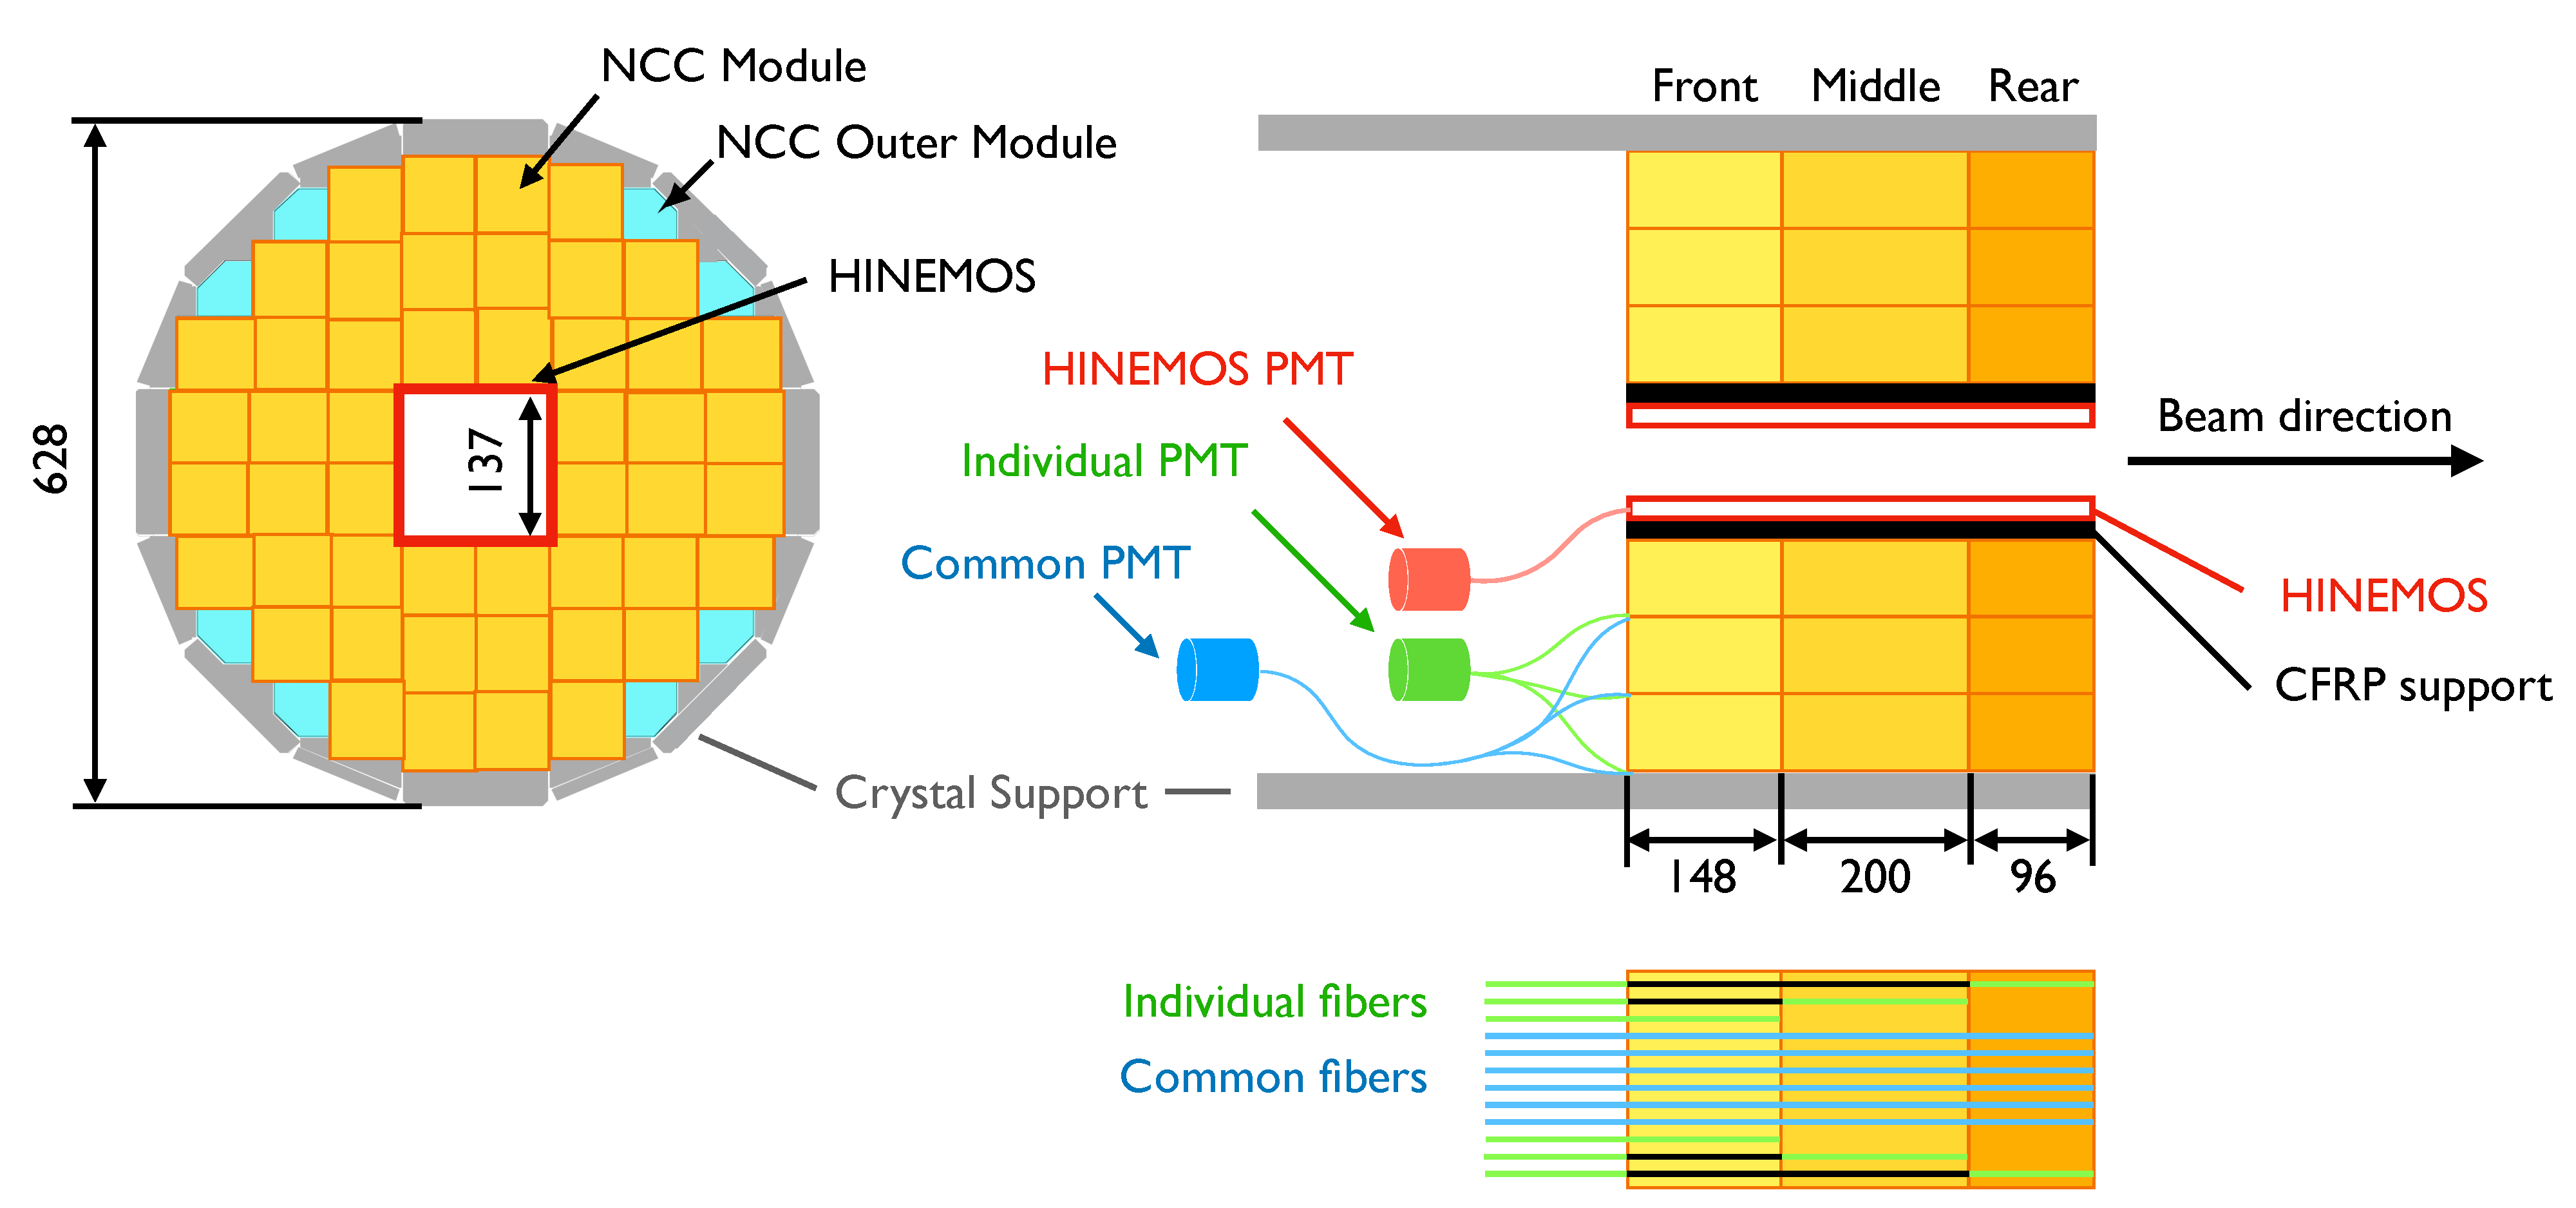
\includegraphics[width=0.99\textwidth]{Figures/Chapter3/NCC_config.pdf}
\caption{A schematic diagram of NCC and HINEMOS \parencite{Maeda, NCC}. The numbers are in the unit of mm.}
\label{fig:NCC_config}
\end{center}
\end{figure}

A $\pi^0$ can also be generated if a $\pi^{\pm}$ penetrates the support installed at the inner surface and undergoes a charge exchange interaction (${\pi^+n \to \pi^0 p}$ or ${\pi^-p \to \pi^0 n}$)\footnote{The source of a single $\pi^{\pm}$ can be produced in the ${K_L^0\to\pi^+\pi^-\pi^0}$ decay at the second collimator. The absence of the coincident hits is expected if other particles do not enter the KOTO detector}. The Horizontal Inner NCC Edge Mounted Scintillator counter (HINEMOS), which consists of four plastic scintillators at the innermost surface, is installed to detect charged particles before the penetration. 

%%
%% 3-6 OEV
%%%%%%%%%%%%%%%%%%%
\subsection{Veto Counters at Outer Edge of the Calorimeter}
The Outer Edge Veto counter (OEV) \parencite{OEV} is composed of 44 lead-scintillator sandwiches with WLS fiber readout. The OEV modules are designed in various shapes appropriately filled in the gap between the cuboid crystals and the cylindrical support of the calorimeter, as shown in Figure~\ref{fig:OEV}. OEV prevents a photon in a $K_L^0$ decay from being absorbed by the support without any detection. 

\begin{figure}[h]
\begin{center}
\captionsetup{width=.99\linewidth}
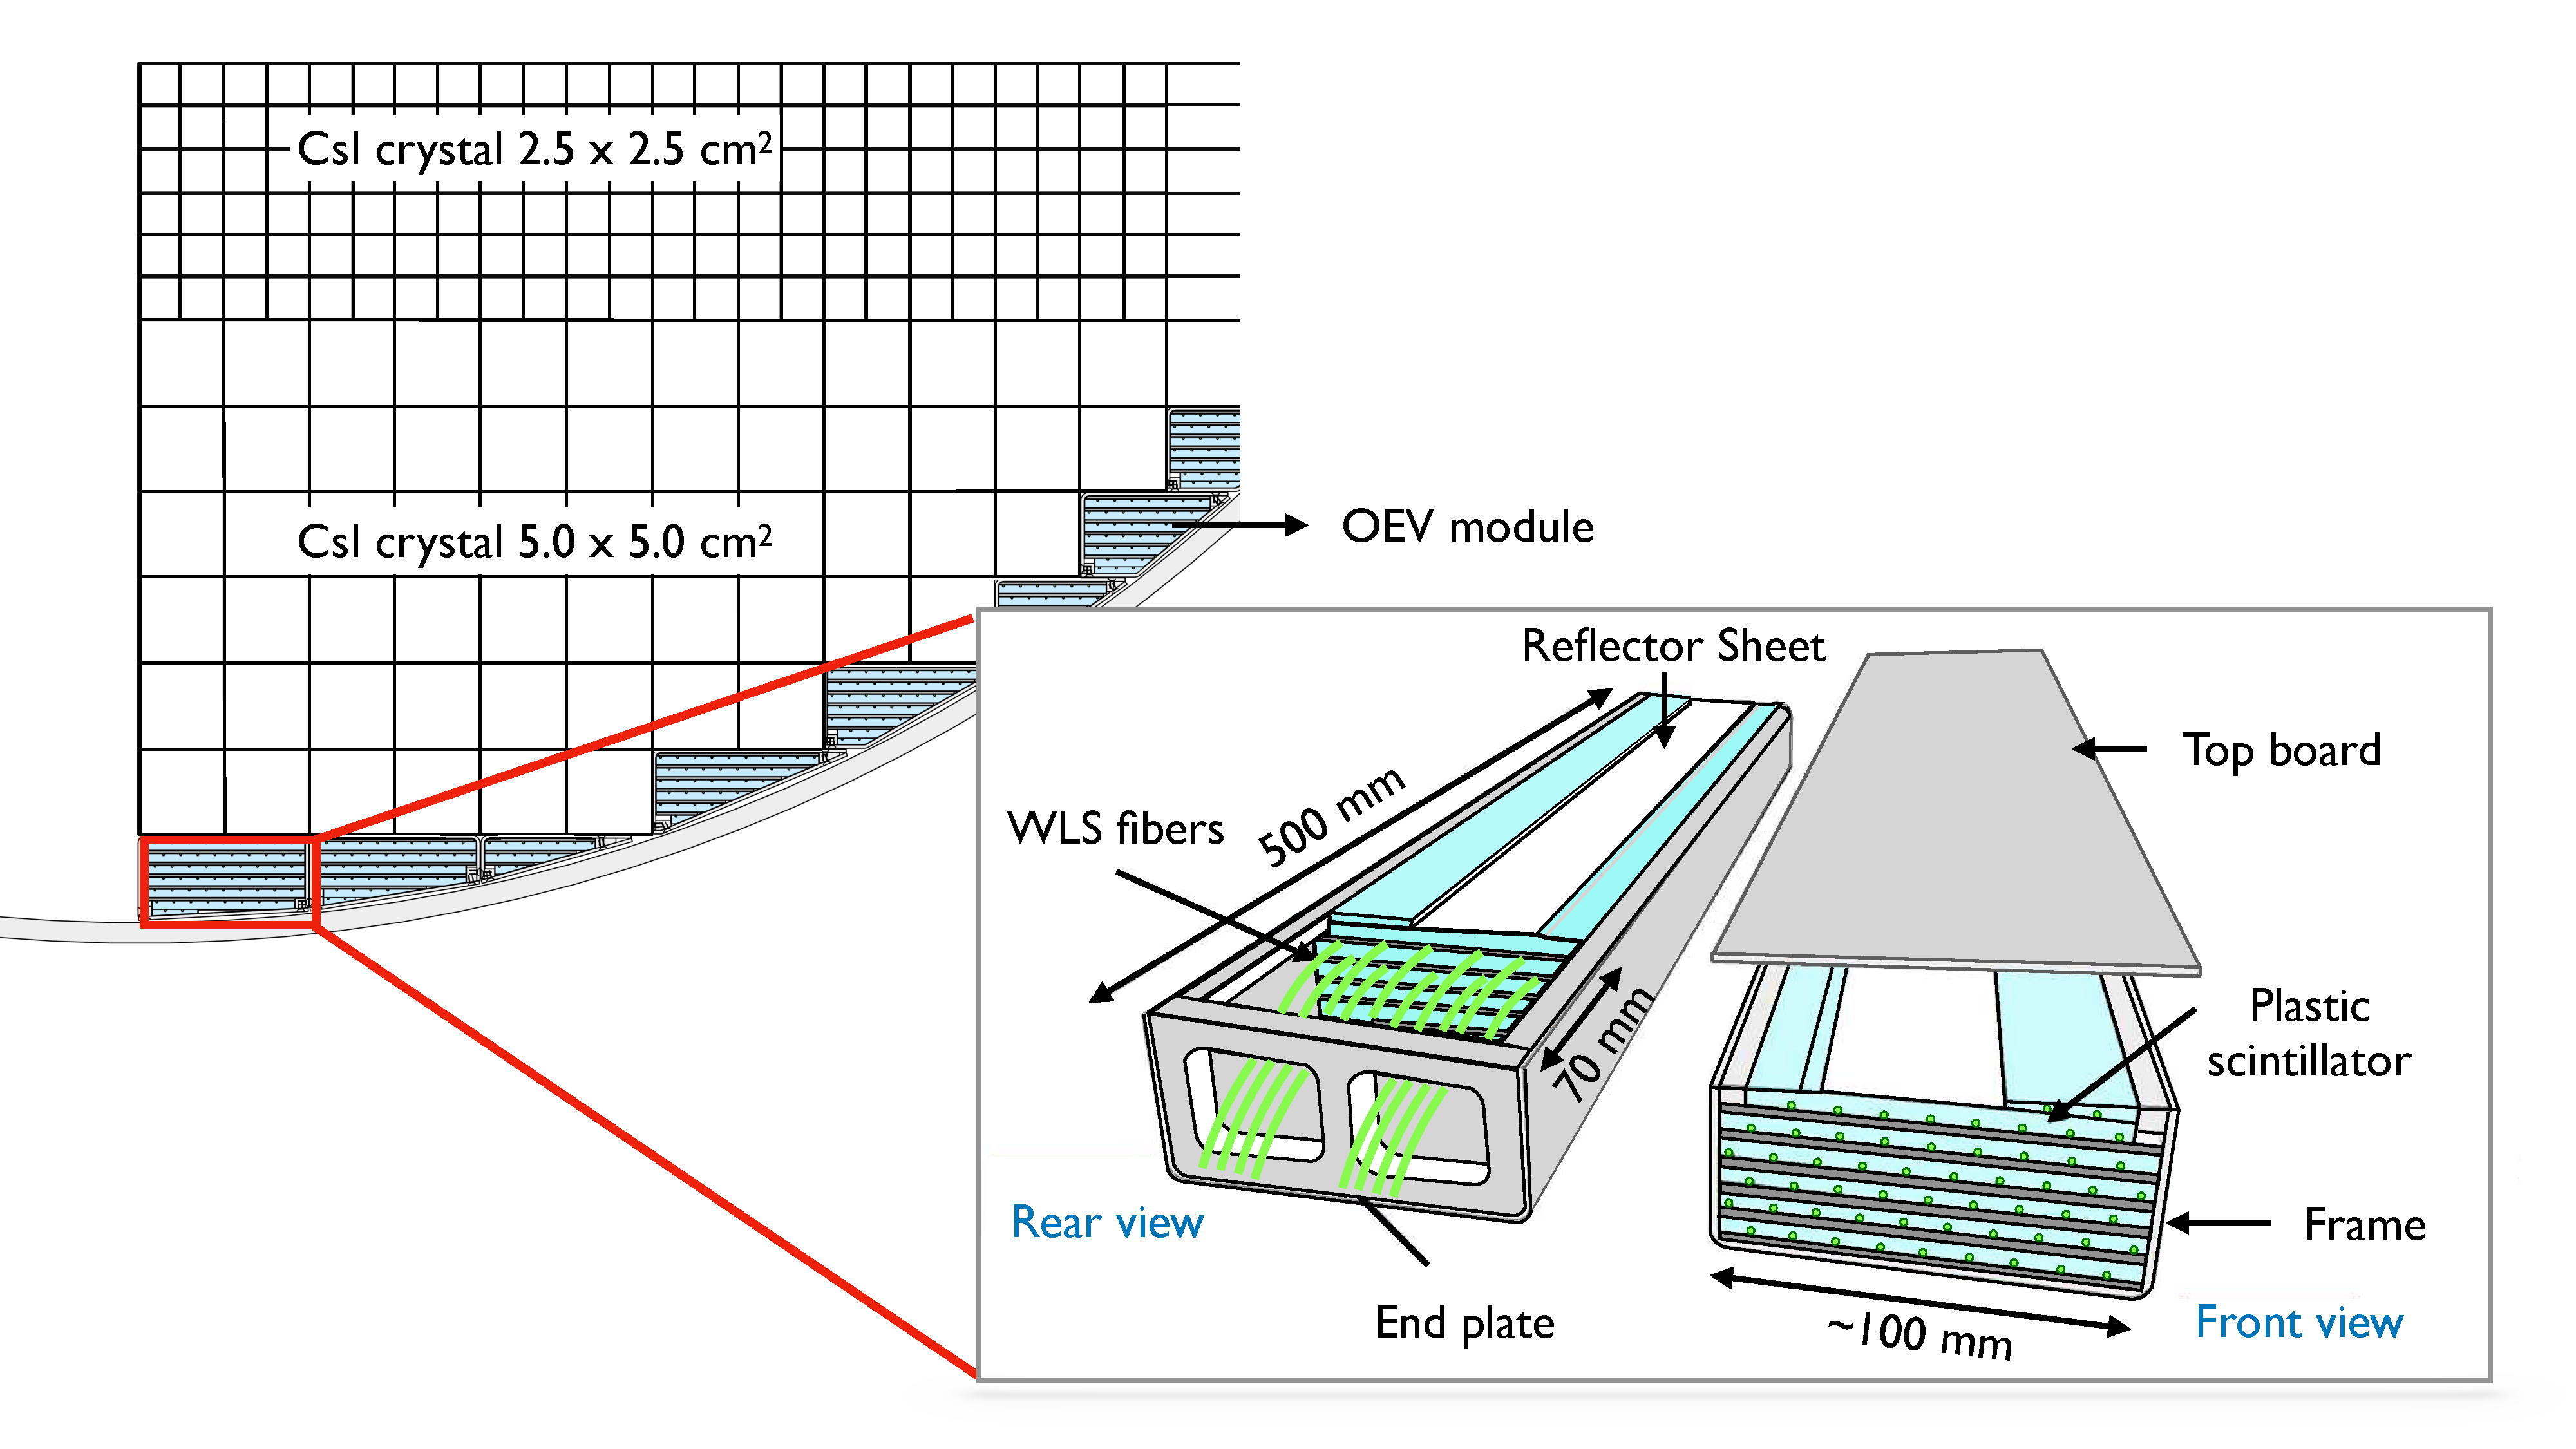
\includegraphics[width=0.99\textwidth]{Figures/Chapter3/OEV_config.pdf}
\caption{A schematic diagram of OEV \parencite{OEV}.}
\label{fig:OEV}
\end{center}
\end{figure}


%%
%% 3-7 CC03, LCV
%%%%%%%%%%%%%%%%%%%%%%

\subsection{Veto Counters inside the Hole of the Calorimeter}
The Collar Counter 3 (CC03) \parencite{CC03} and the Linear Charged Veto counter (LCV) \parencite{LCV} are the square-tube counters inside the hole of the calorimeter for detecting any photons or charged particles hitting around. Figure~\ref{fig:CC03_LCV} shows the configuration of CC03 and LCV. The beam pipe, a 4.5-mm-thick CFRP tube, is installed along the hole for maintaining the whole structure. CC03 consists of sixteen undoped cesium iodide crystals stacked between the calorimeter and the beam pipe. These crystals are not involved in the photon reconstruction in the calorimeter but detects any extra activities near the beam hole. LCV is composed of four 3-mm-thick plastic scintillators embedded with WLS fibers and attached at the inner surface of the beam pipe for detecting a charged particle before entering the beam pipe. Notably, LCV is further extended upstream to CV for the complete coverage.

\begin{figure}[h]
\begin{center}
\captionsetup{width=.99\linewidth}
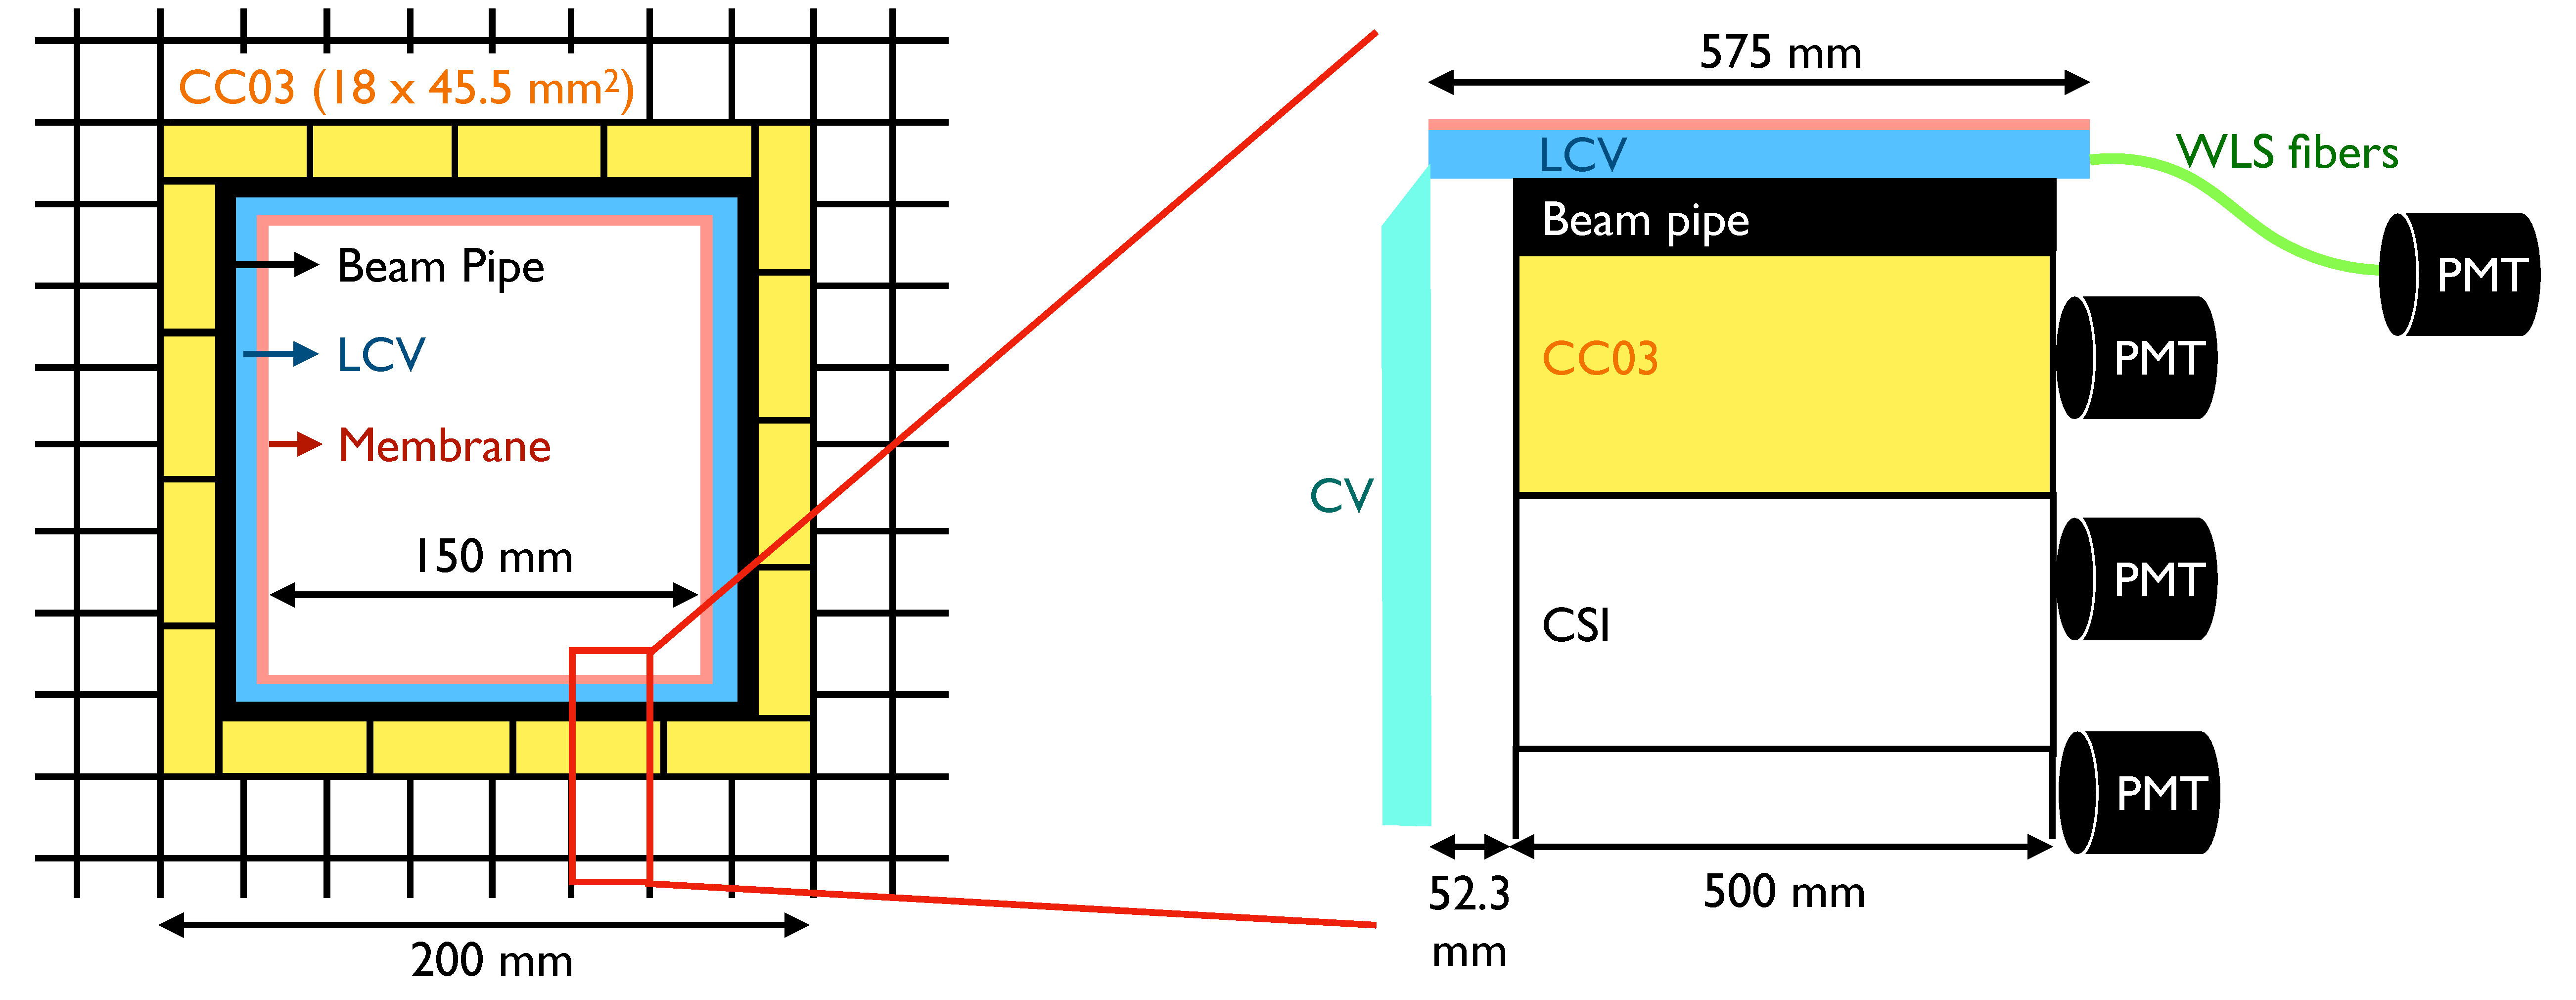
\includegraphics[width=0.85\textwidth]{Figures/Chapter3/CC03_LCV.pdf}
\caption{A schematic diagrams of CC03 and LCV \parencite{Maeda}.}
\label{fig:CC03_LCV}
\end{center}
\end{figure}

%% 
%% 3-8 Downstream collar counter CC04 - CC06
%%%%%%%%%%%%%%%%%%%%%%%%%%%%%%%%%%%%%%%%%%%

\subsection{Downstream Collar Counters}
In the downstream region of the calorimeter, three collar counters, abbreviated as CC04, CC05, and CC06, are installed perpendicularly to the beam direction \parencite{CC04_CC06}.  As Figure~\ref{fig:CC0X} shows, the beam pipe, a 5-mm-thick aluminum square tube, is constructed along the beam hole as an extension of the vacuum environment. CC04 lies inside the vacuum tank, CC05 is installed around the beam pipe, and CC06 is placed in the downstream region of the beam pipe exit. The three collar counters are all composed of undoped Cesium Iodide crystals and the plastic scintillators at upstream surface for detecting photons and charged particles respectively. 

\begin{figure}[H]
\begin{center}
\captionsetup{width=.99\linewidth}
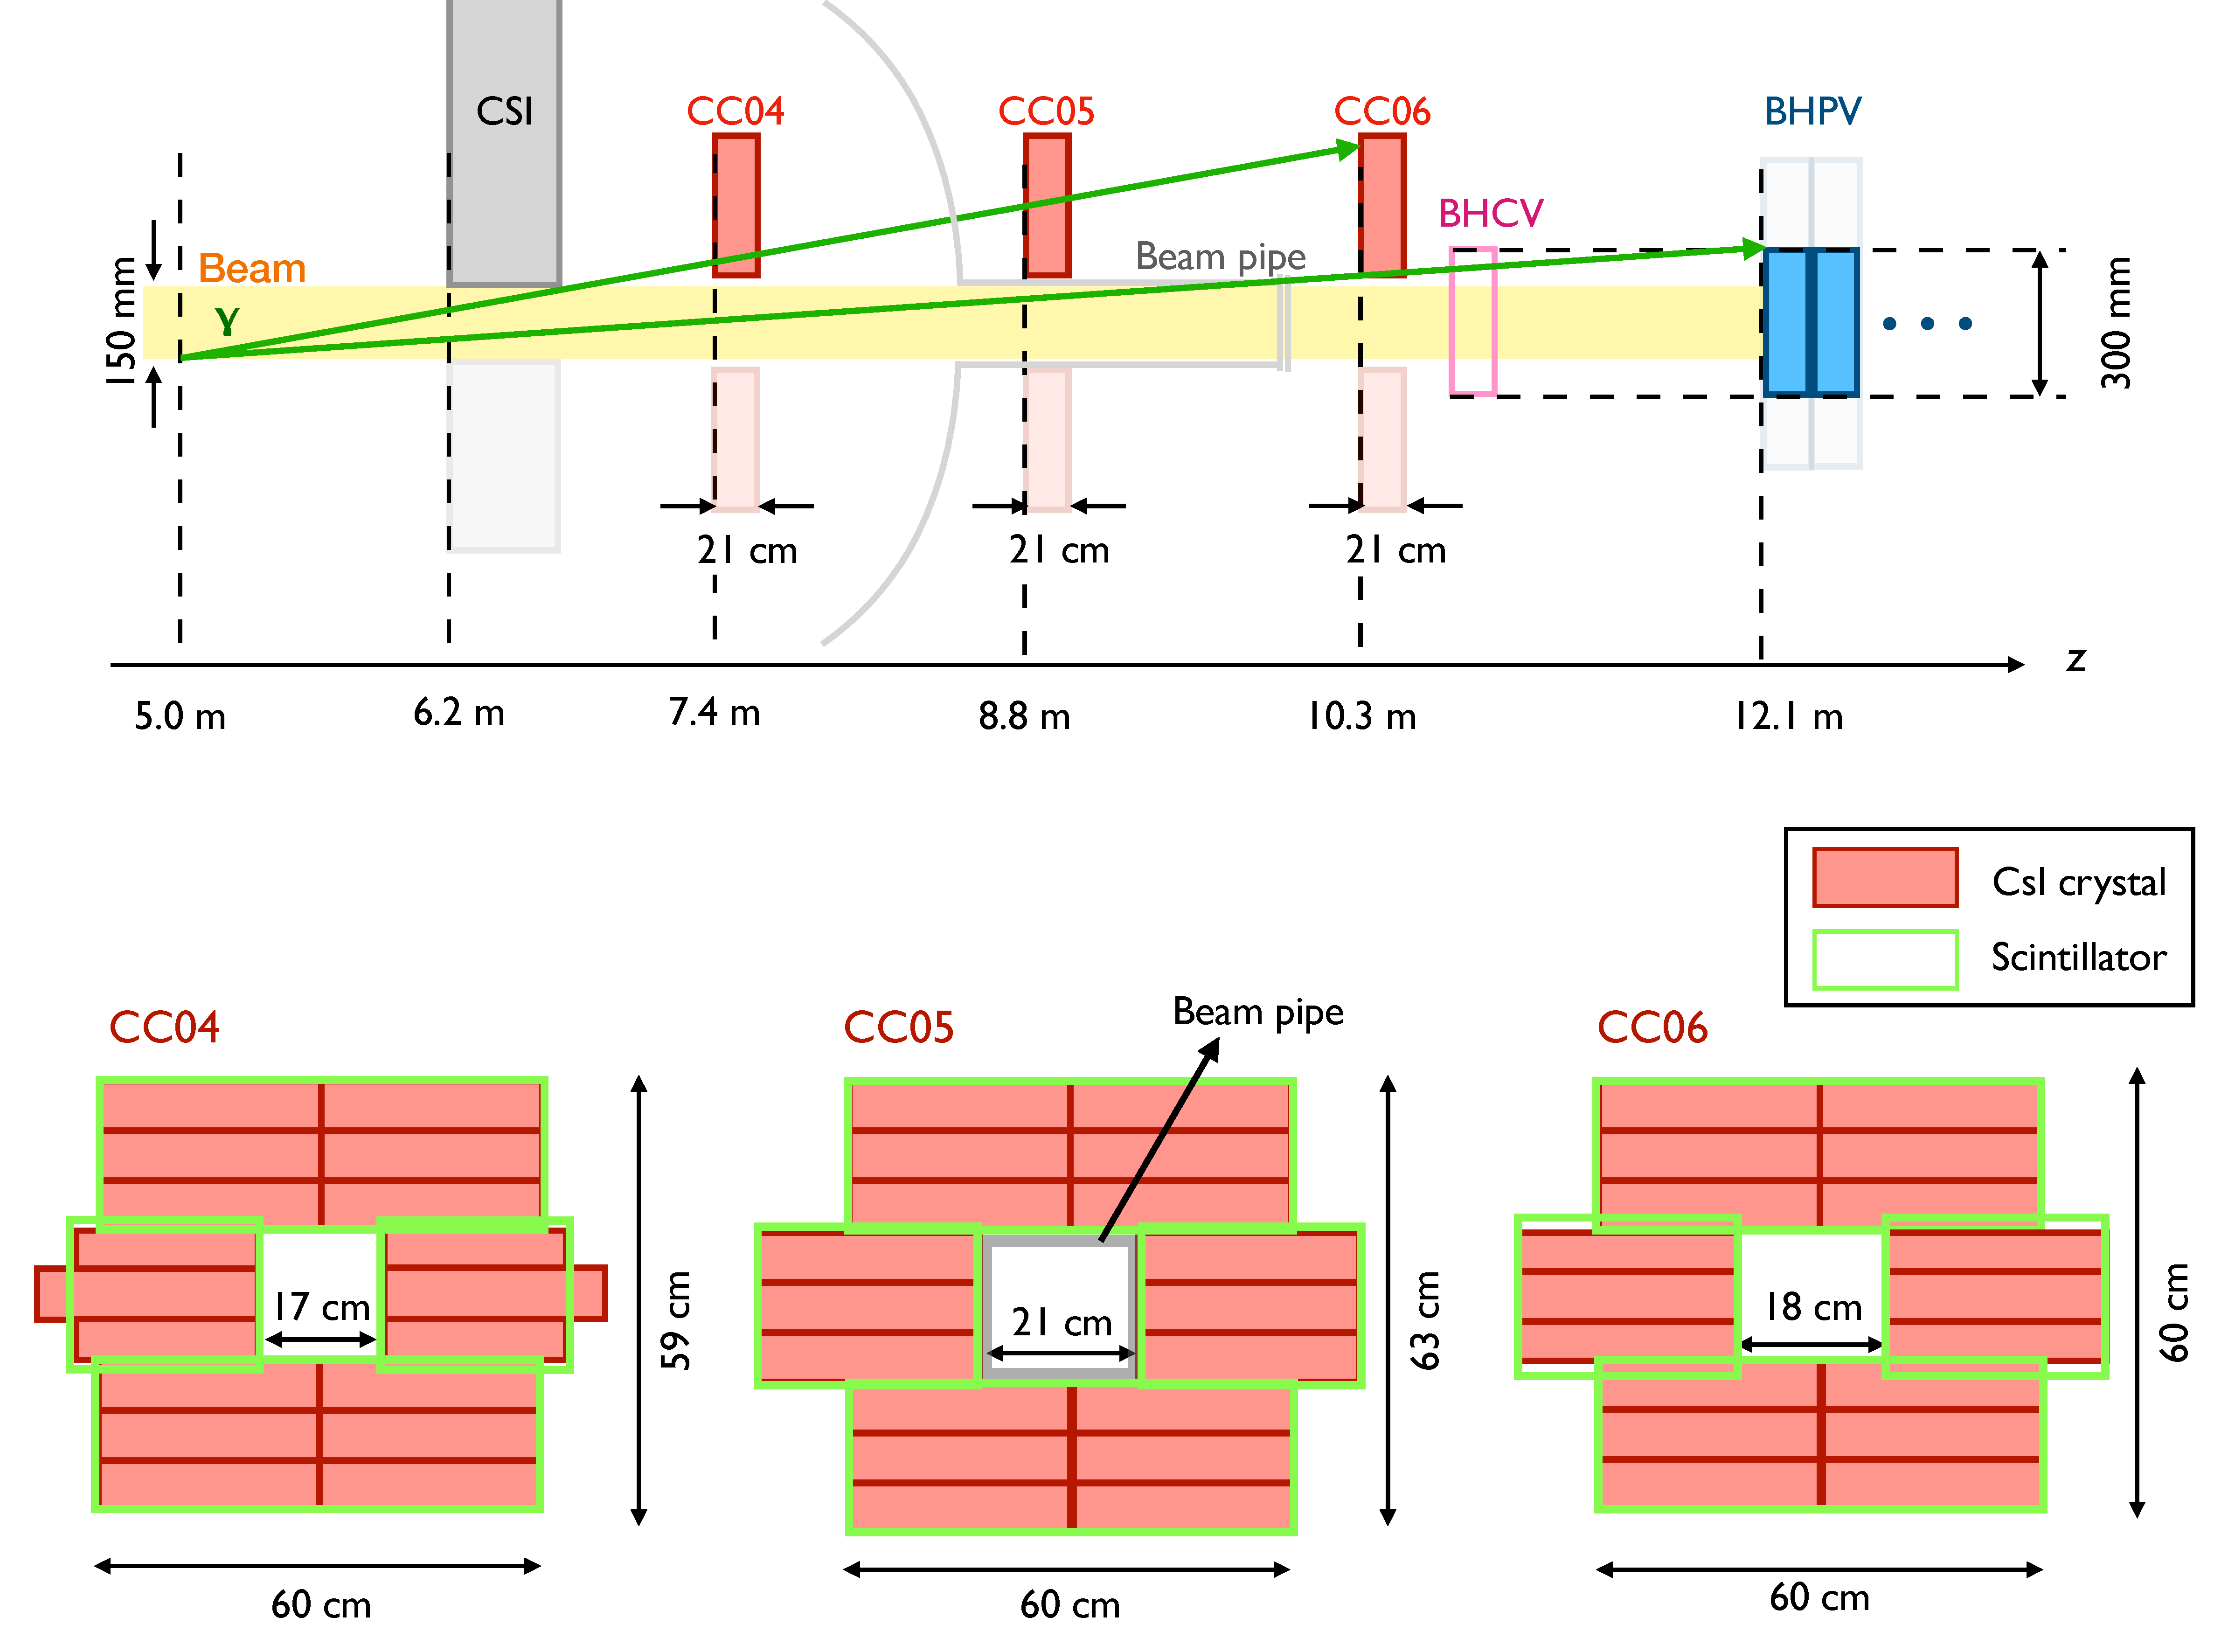
\includegraphics[width=0.99\textwidth]{Figures/Chapter3/CC04_CC06.pdf}
\caption{A schematic diagram of CC04, CC05, and CC06 \parencite{CC04_CC06}. The two green lines indicate the coverage of the downstream counters to a photon from the edge of the beam at z~$=$~5~m. BHPV and BHCV are the in-beam photon and charged particle veto counters respectively (explained in Section~\ref{sec:beam_hole_counter}).} 
\label{fig:CC0X}
\end{center}
\end{figure}

By assuming the downstream boundary of a signal candidate is z~$=$~5~m, the location of CC06 ensures any photon in the ${K_L^0\to\pi^0\pi^0}$ decay escaping into the beam hole can be detected by any of the downstream counters. In line with this, a $\pi^{\pm}$ in the ${K_L^0\to\pi^+\pi^-\pi^0}$ is in general nowhere to escape.

%%
%% 3-9 Beam pipe charge veto (BPCV)
%%%%%%%%%%%%%%%%%%%%%%%%%%%%%%%%%%%%%%%

\subsection{Beam Pipe Charge Veto Counter} 

The ${K_L^0\to\pi^+\pi^-\pi^0}$ decay can be a serious background source if the $\pi^{\pm}$s are absorbed by the beam pipe before entering CC06. The Beam Pipe Charge Veto (BPCV) counter \parencite{BPCV}, which is composed of four 5-mm-thick plastic scintillators surrounding the beam pipe, is therefore implemented to further enhance the detection capability of $\pi^{\pm}$s, as shown in Figure \ref{fig:BPCV}. 

\begin{figure}[H]
\begin{center}
\captionsetup{width=.99\linewidth}
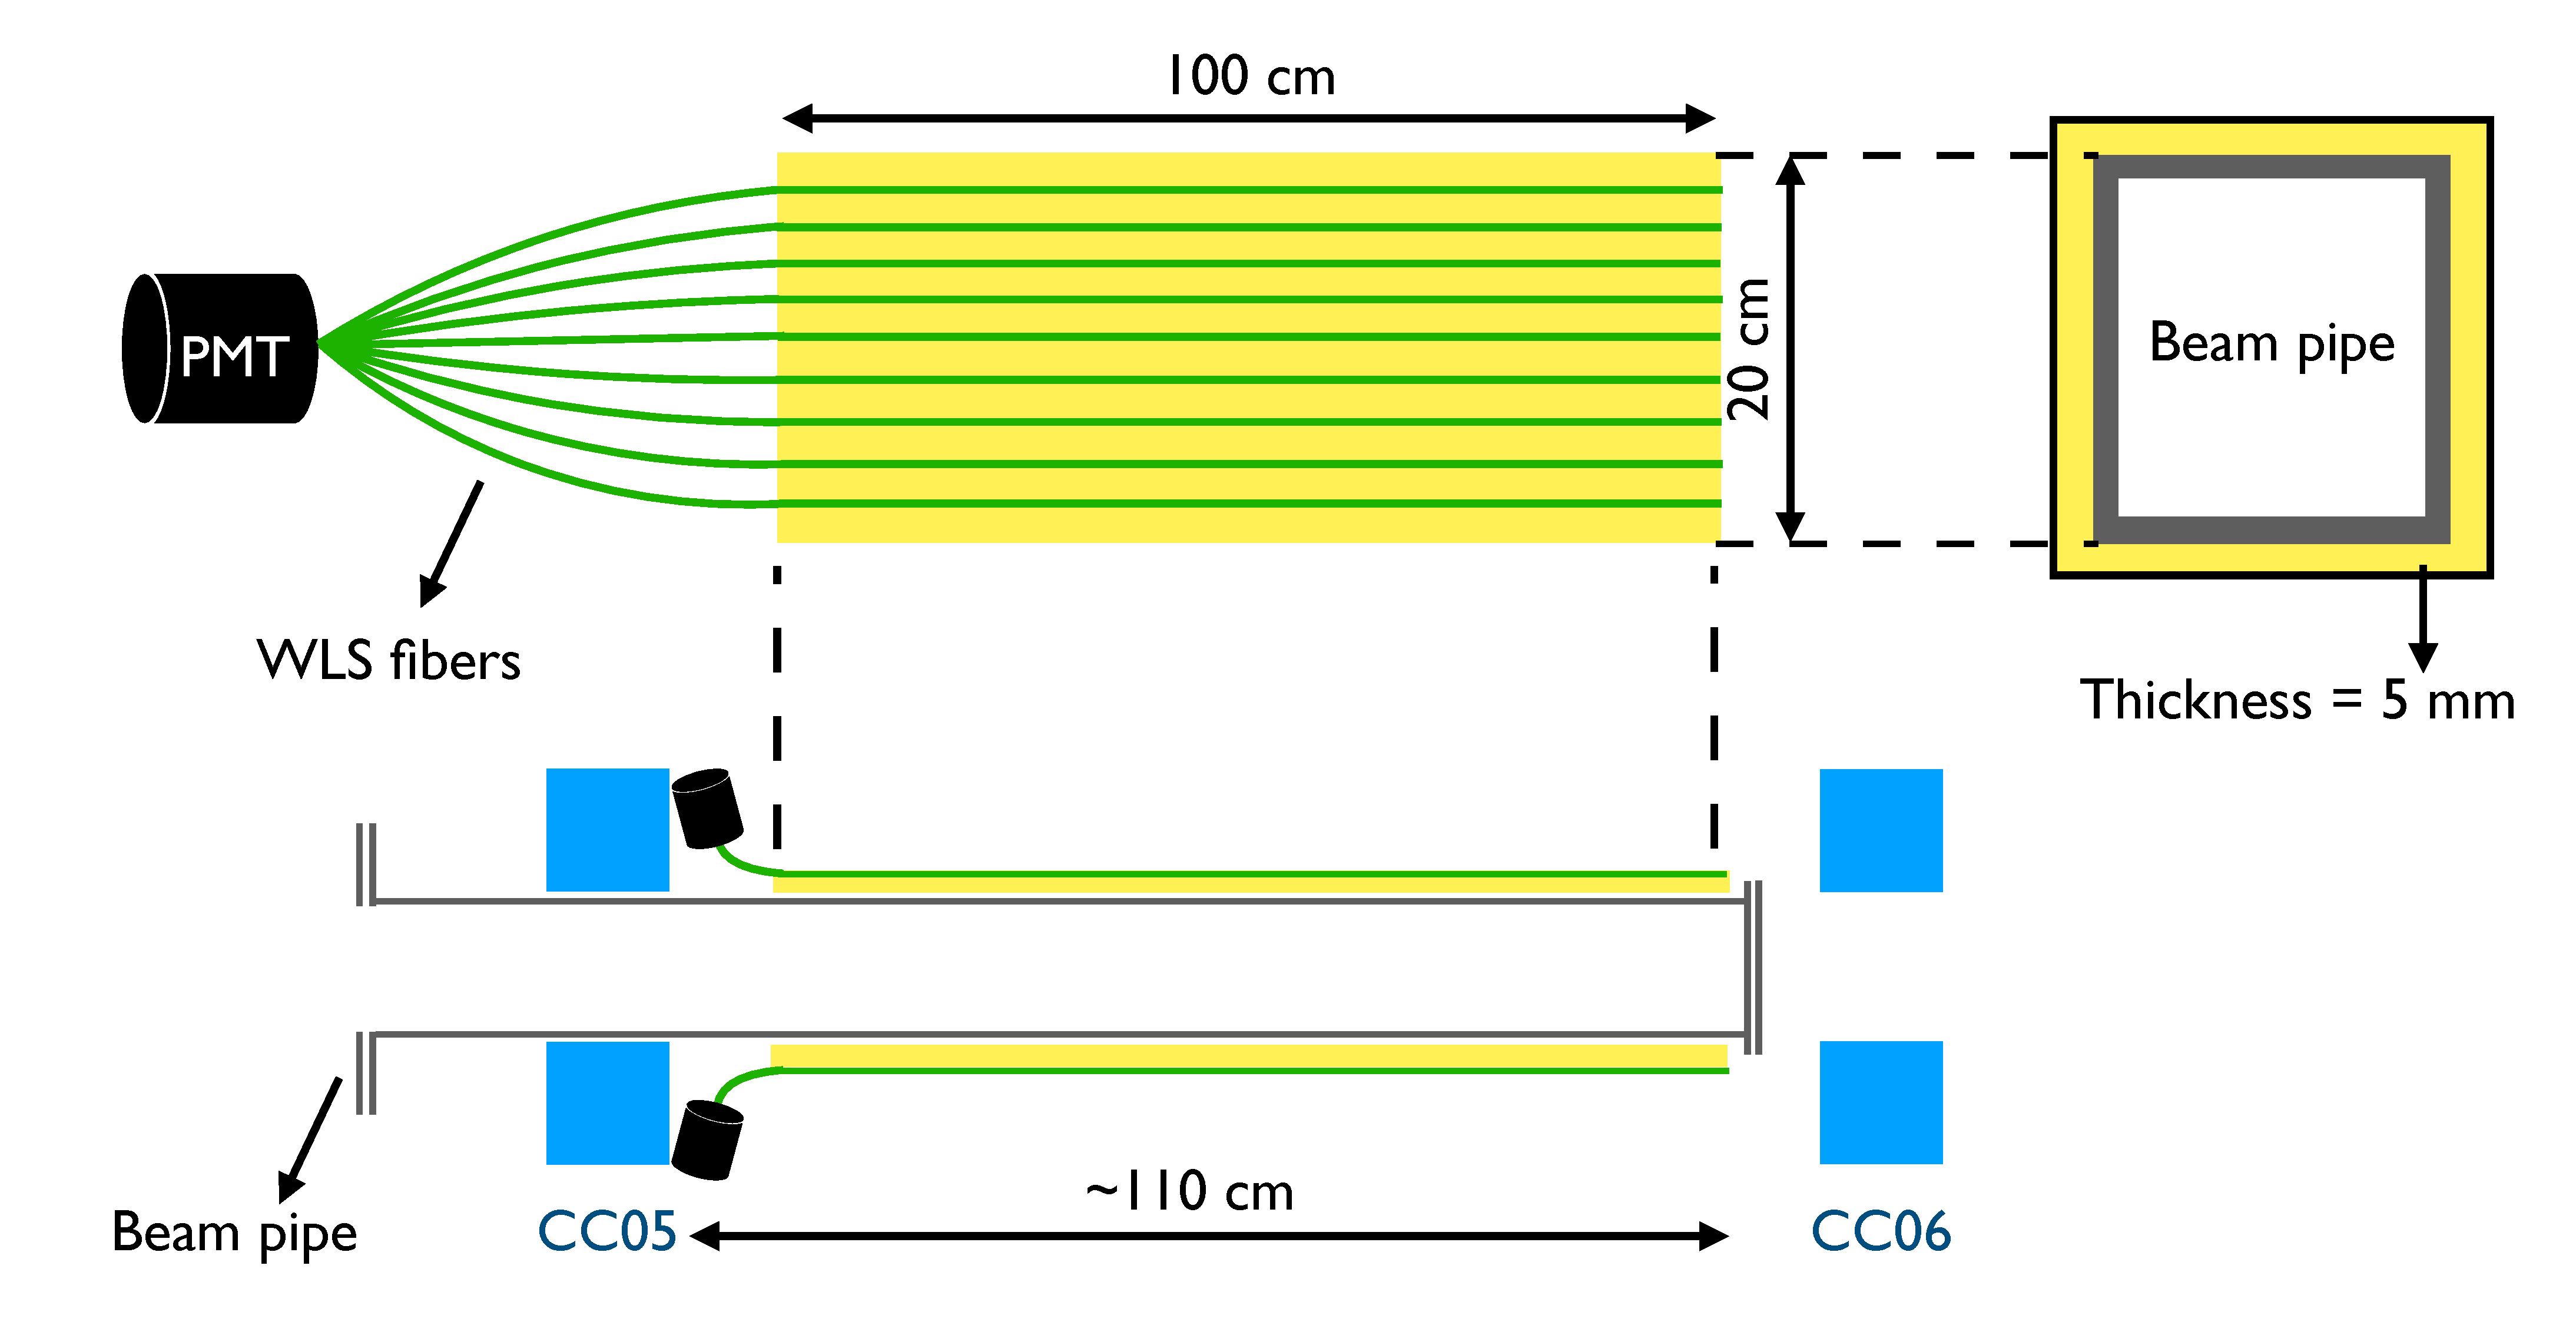
\includegraphics[width=0.9\textwidth]{Figures/Chapter3/BPCV.pdf}
\caption{A schematic diagram of BPCV \parencite{BPCV}.}
\label{fig:BPCV}
\end{center}
\end{figure}

%
%% 3-10 Beam hole counters
%%%%%%%%%%%%%%%%%%%%%%%%%%%
\subsection{Beam Hole Veto Counters}
\label{sec:beam_hole_counter}
The in-beam veto counters are located at the end of the KOTO detector, which are regarded as the last-ditch attempt to capture the extra particles in a $K_L^0$ decay traveling along the beam. These counters typically suffer from the numerous neutrons in the beam and needs to tolerate the high-rate environment. As a result, the balance between the neutron insensitivity and the detection power of the escaping particles is a crucial topic for designing beam hole counters.

\subsubsection{Charge veto at beam hole}
The Beam Hole Charge Veto (BHCV) counter \parencite{BHCV, BHCV2}, a multi-wire chamber filled with mixed gas of Tetrafluoromethane (CF4) and n-Pentane, is primarily constructed at the beam region to detect $\pi^{\pm}$s in the ${K_L^0 \to \pi^+ \pi^- \pi^0}$ decay. Figure~\ref{fig:BHCV} describes the principle of BHCV. When a charged particle passes through the chamber, the surrounding gas is ionized into ions and electrons. Under the influence of the electric field, the resulting charges are collected through the wires and cause the pulses. 

BHCV features the thin gap between the wires and the planes, which enable the rapid response to the gaseous ionization. Moreover, the light materials are utilized to eliminate the interactions with the neutrons and the photons contained in the beam. BHCV has three modules in a row along the beam. The coincident signals in more than two consecutive modules are required to reduce the noise.

\begin{figure}[h]
\begin{center}
\captionsetup{width=.99\linewidth}
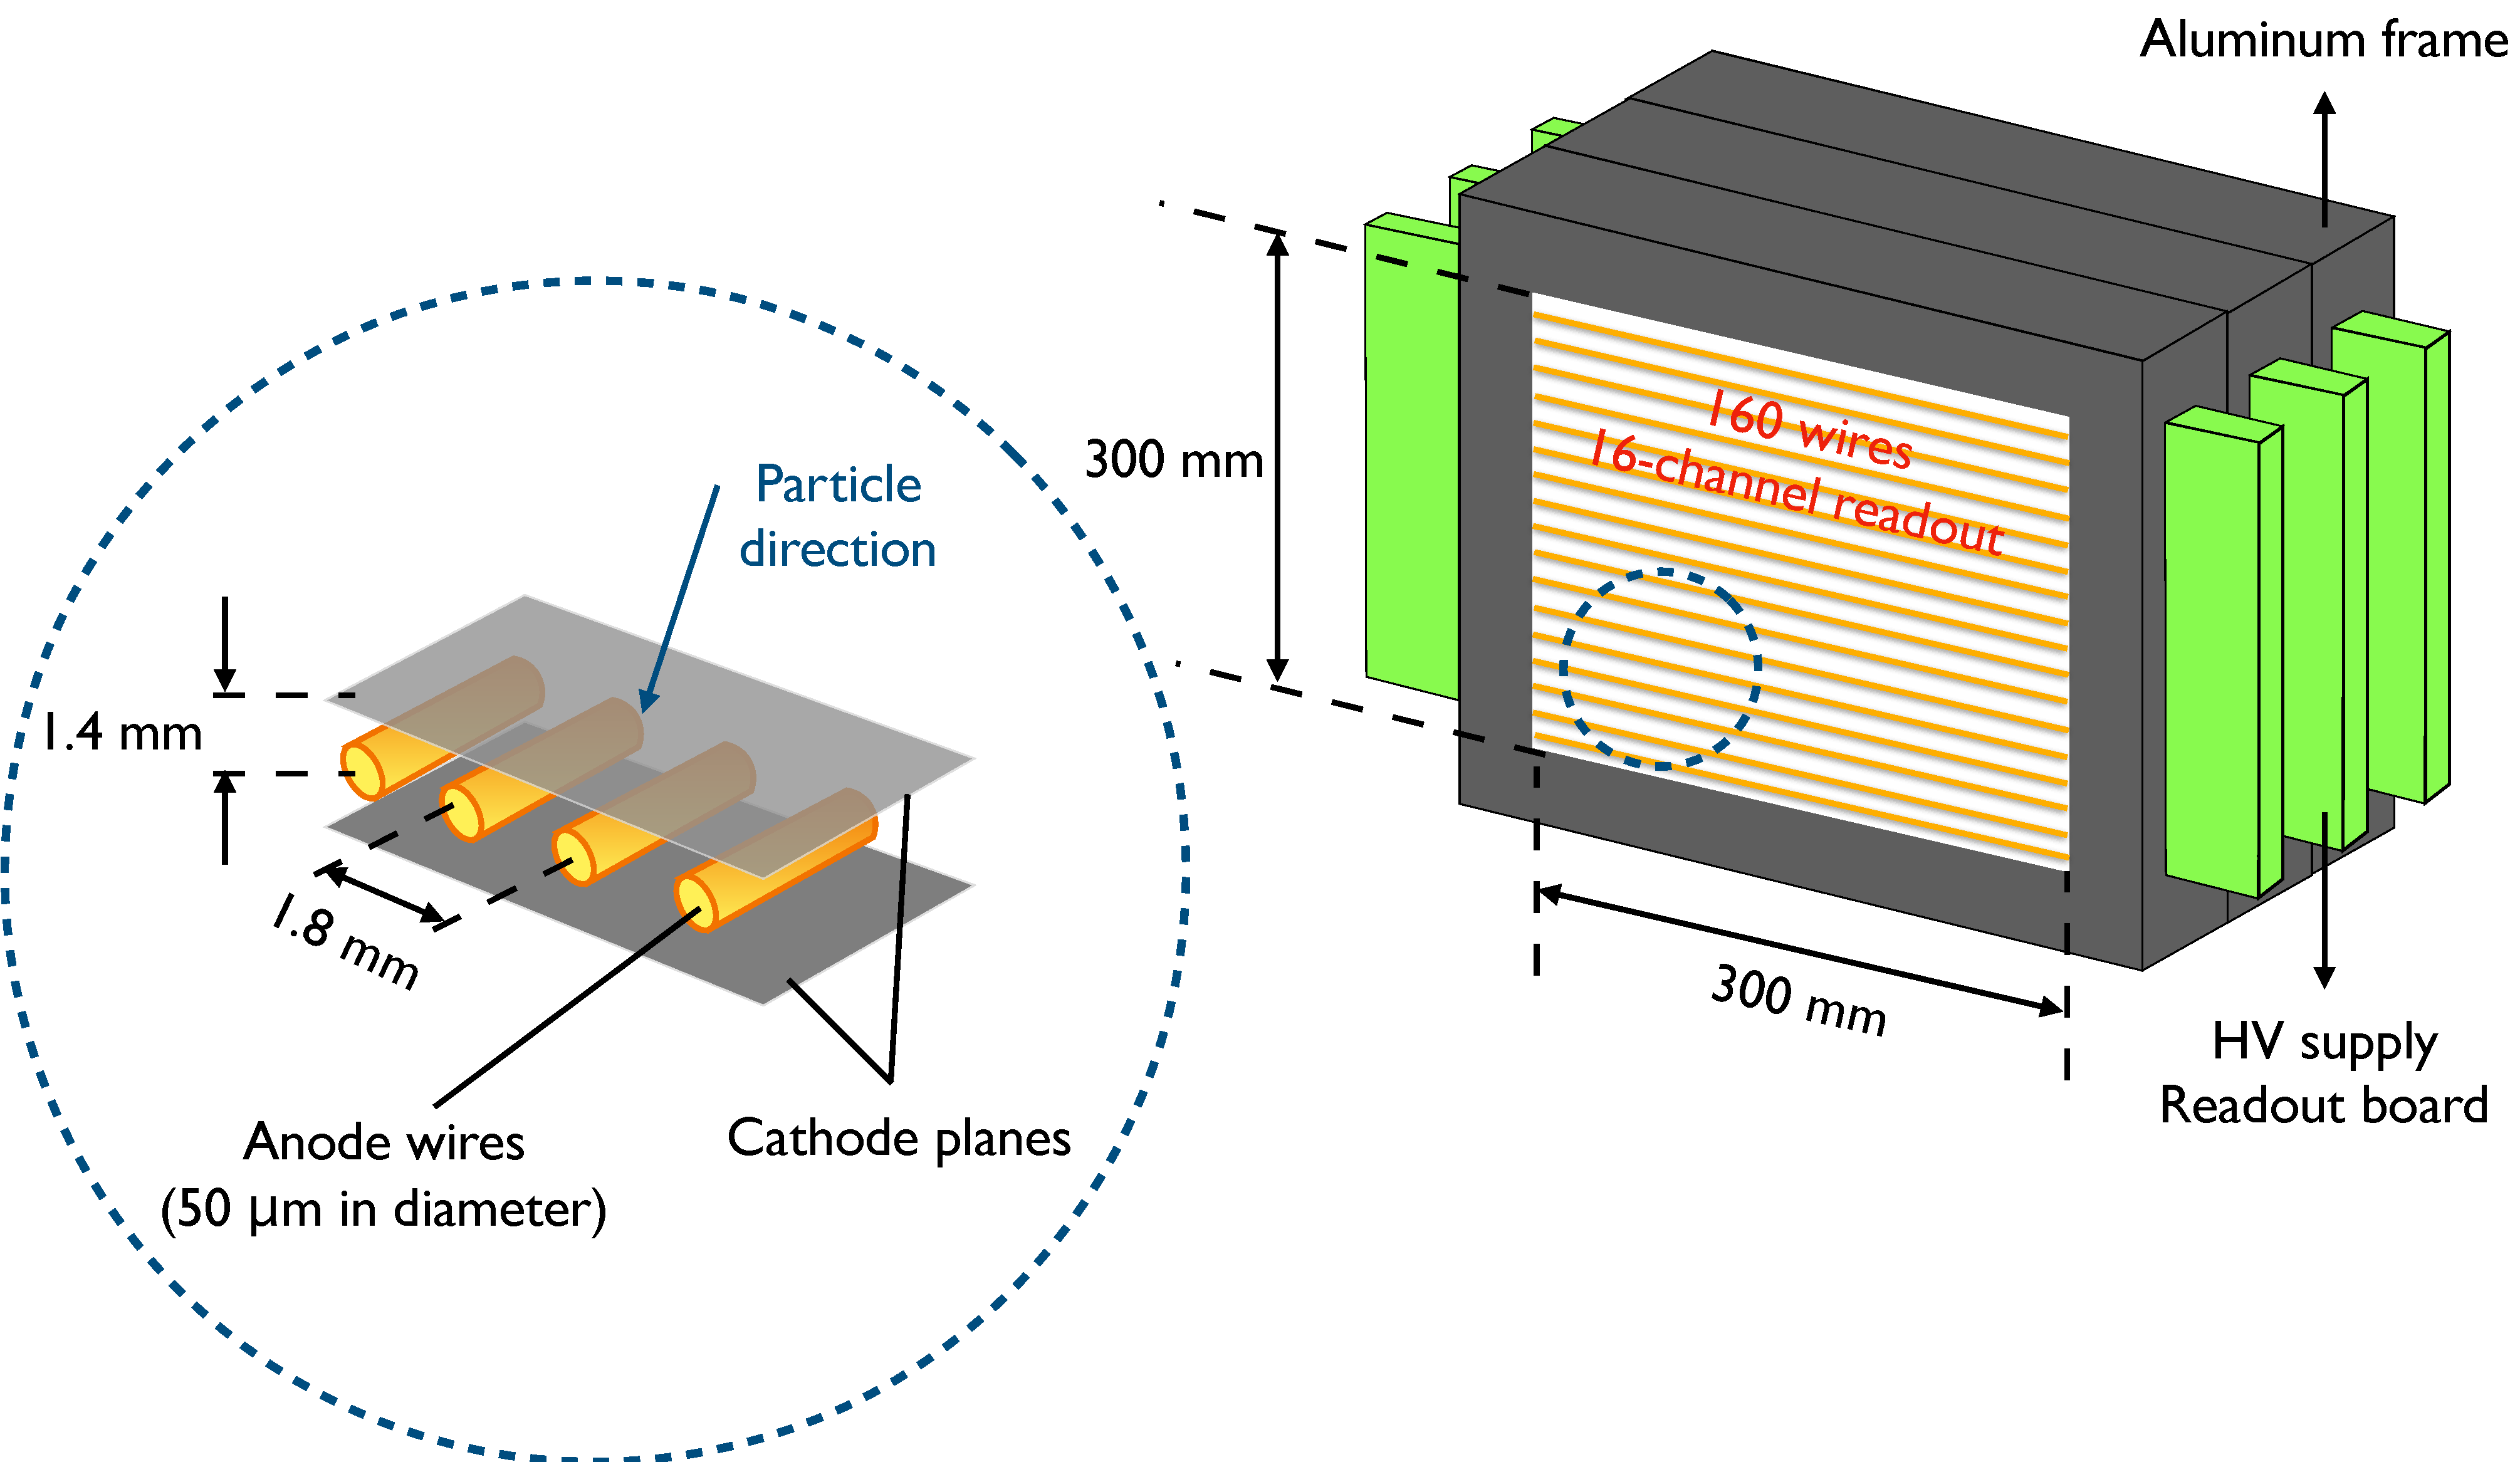
\includegraphics[width=0.99\textwidth]{Figures/Chapter3/BHCV.pdf}
\caption{A schematic diagram of BHCV \parencite{BHCV}.}
\label{fig:BHCV}
\end{center}
\end{figure}


%\begin{figure}[h]
%\begin{center}
%\captionsetup{width=.99\linewidth}
%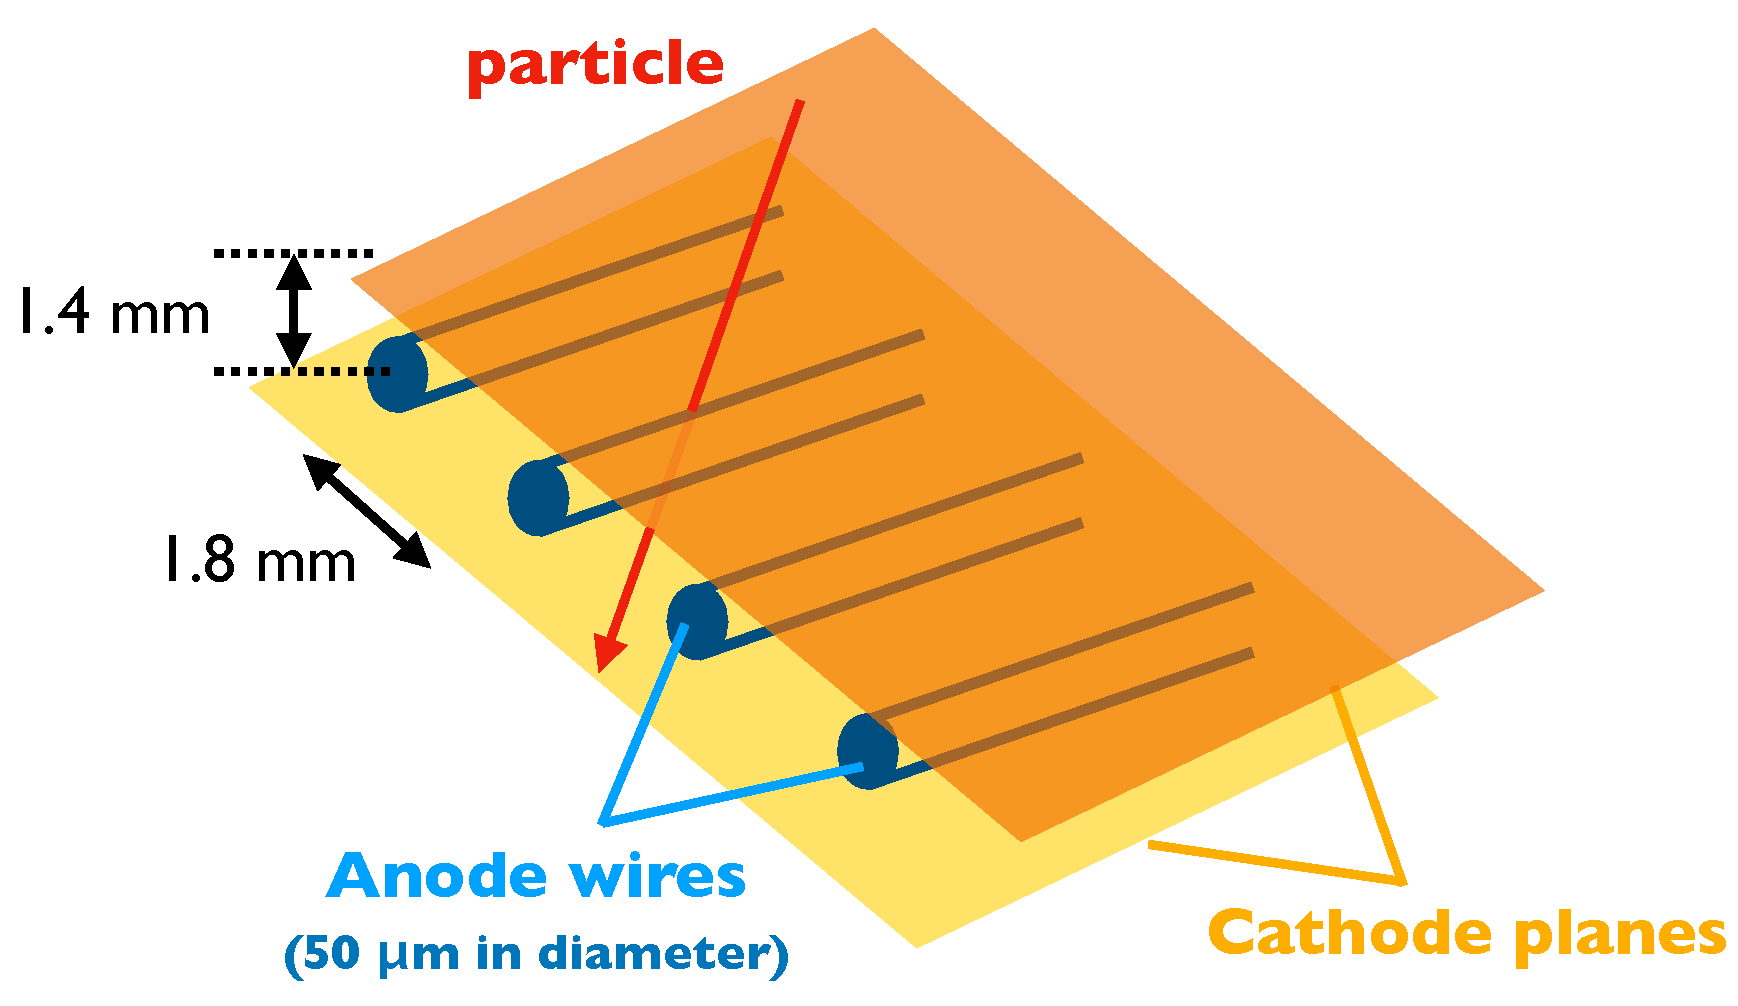
\includegraphics[width=0.7\textwidth]{Figures/Chapter3/BHCV_schematic.pdf}
%\caption{Principle of a ulti-wire chamber for BHCV.}
%\label{fig:BHCV_schematic}
%\end{center}
%\end{figure}


%\begin{figure}[h]
%\begin{center}
%\captionsetup{width=.99\linewidth}
%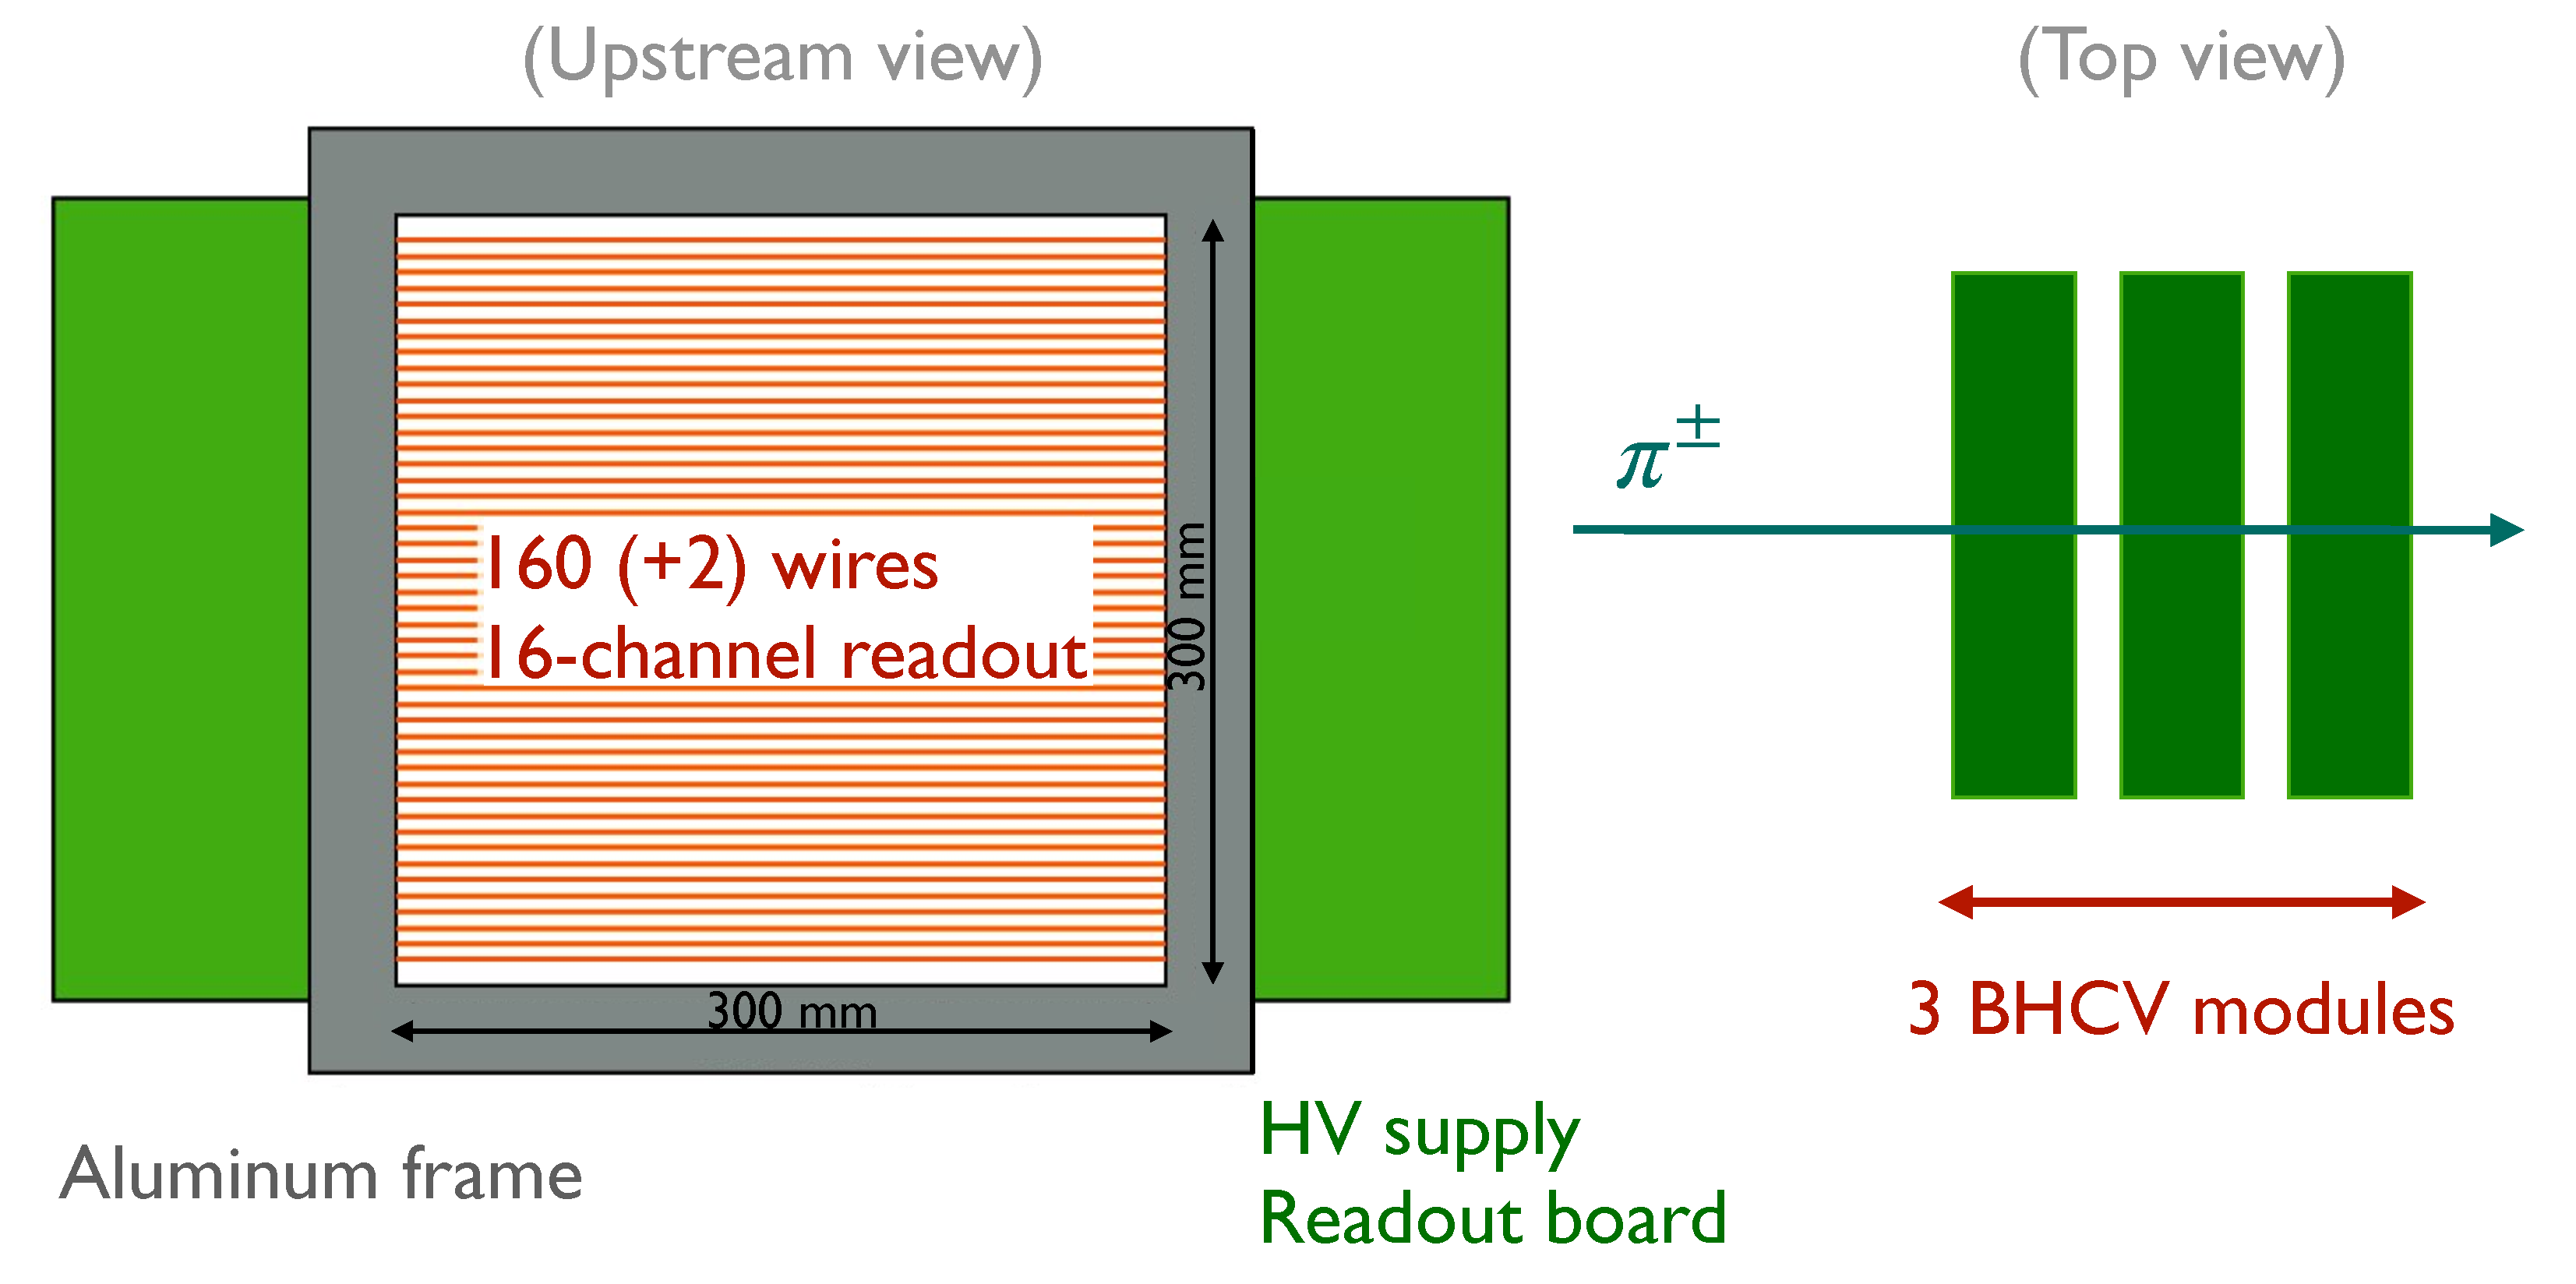
\includegraphics[width=0.8\textwidth]{Figures/Chapter3/BHCV_config.pdf}
%\caption{A graphical illustration of BHCV (Figure courtesy of \parencite{BHCV} with modifications).}
%\label{fig:BHCV_config}
%\end{center}
%\end{figure}

\subsubsection{Photon veto at beam hole}
If one of the photons in a $\pi^0\to2\gamma$ decay is too soft, the other tends to boost forward and escape into the beam hole. Because soft photons are barely detectable, the sensitivity to the energetic photons in the beam translates into the background level, especially for the ${K_L^0 \to \pi^0 \pi^0}$ background. The two subdetectors, Beam Hole Photon Veto (BHPV) \parencite{BHPV} and Beam Hole Guard Counter (BHGC) \parencite{BHGC}, are \v{C}erenkov counters for photon veto. As Figure \ref{fig:BHPV_BHGC} shows, an energetic photon strikes a lead converter and produces an electron-positron pair. The \v{C}erenkov light is then radiated by the material (an aerogel tile for BHPV or an acrylic plate for BHGC), guided to either side of the module, and collected by a PMT.  In contrast, a \v{C}erenkov light is scarcely produced by slow-neutrons because the generated charged particle tends to be slower than the speed of light in the material.

BHPV is the in-beam counter that consists of 16 modules in a row and BHGC is the beam-edge counter to complement the photon detection. A concrete shield is implemented in front of BHPV to eliminate the shower splashing back to its upstream counters. Both BHPV and BHGC possess an approach to further suppress the fake signals due to the \v{C}erenkov light induced by slow neutrons. BHPV requires the coincident signals in consecutive modules, because the electromagnetic shower developed by energetic photons tends to spread forward, while the secondary particles from slow-neutron interactions tend to propagate isotropically. BHGC inhibits the \v{C}erenkov light transmitting along the plate if the resulting angle is smaller than the critical angle.

%\begin{figure}[h]
%\begin{center}
%\captionsetup{width=.99\linewidth}
%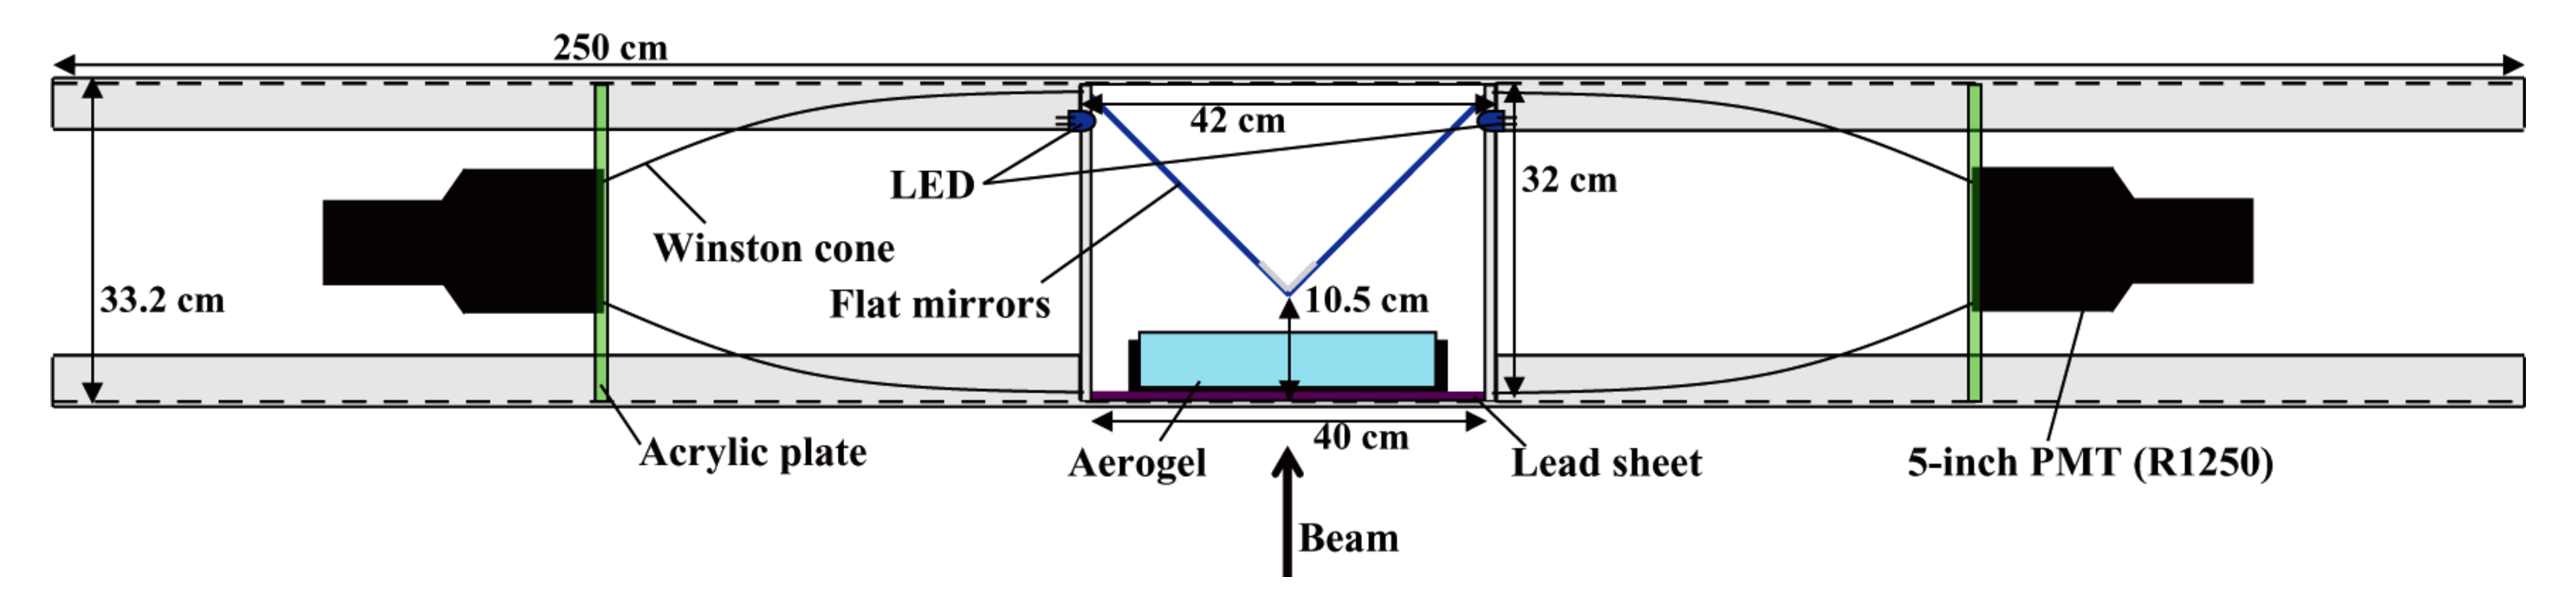
\includegraphics[width=0.9\textwidth]{Figures/Chapter3/BHPV_module.pdf}
%\caption{A schematic diagram of a BHPV module (Figure courtesy of \parencite{BHPV}).}
%\label{fig:BHPV_module}
%\end{center}
%\end{figure}

%\begin{figure}[h]
%\begin{center}
%\captionsetup{width=.99\linewidth}
%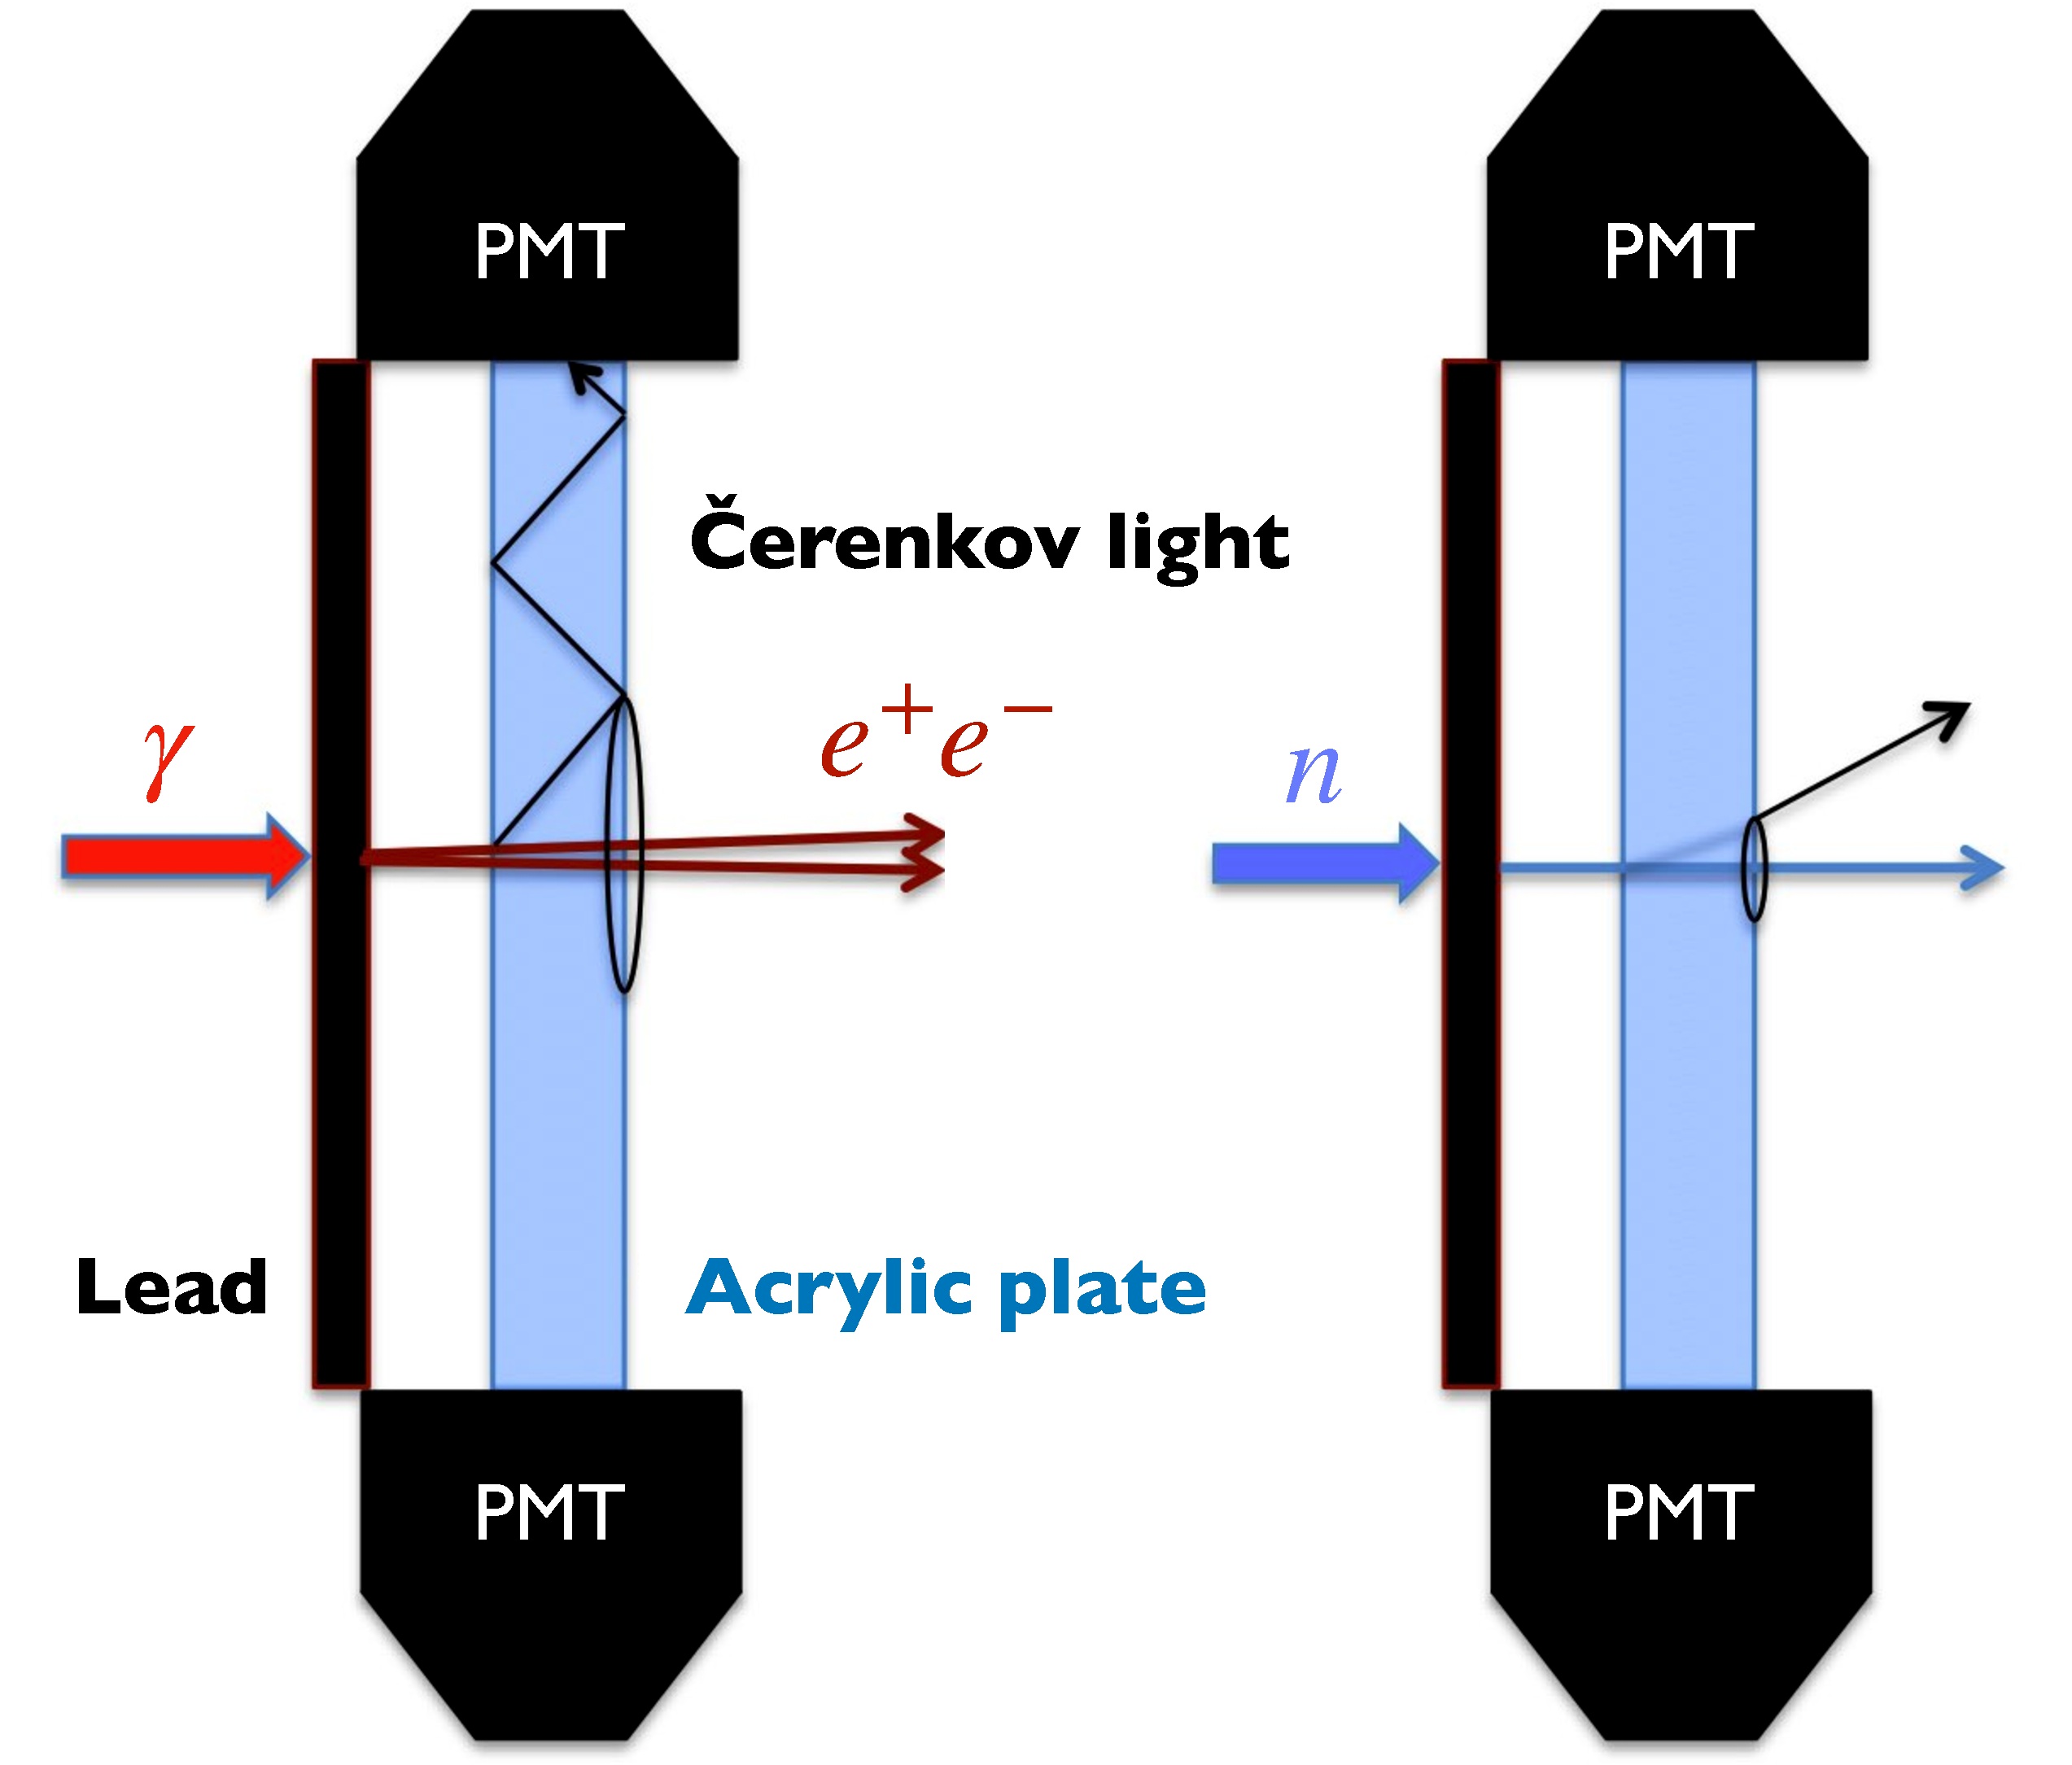
\includegraphics[width=0.5\textwidth]{Figures/Chapter3/BHGC_principle.pdf}
%\caption{Particle responses at BHGC (Figure courtesy of \parencite{BHGC2}).}
%\label{fig:BHGC_principle}
%\end{center}
%\end{figure}

%BHPV is the in-beam counter that consists of 16 modules in a row and BHGC is the beam-edge counter to complement the photon detection, as shown in Figure \ref{fig:BHPV_BHGC}. A concrete shield is implemented in front of BHPV to eliminate the shower splashing back to its upstream counters.

%\begin{figure}[h]
%\begin{center}
%\captionsetup{width=.99\linewidth}
%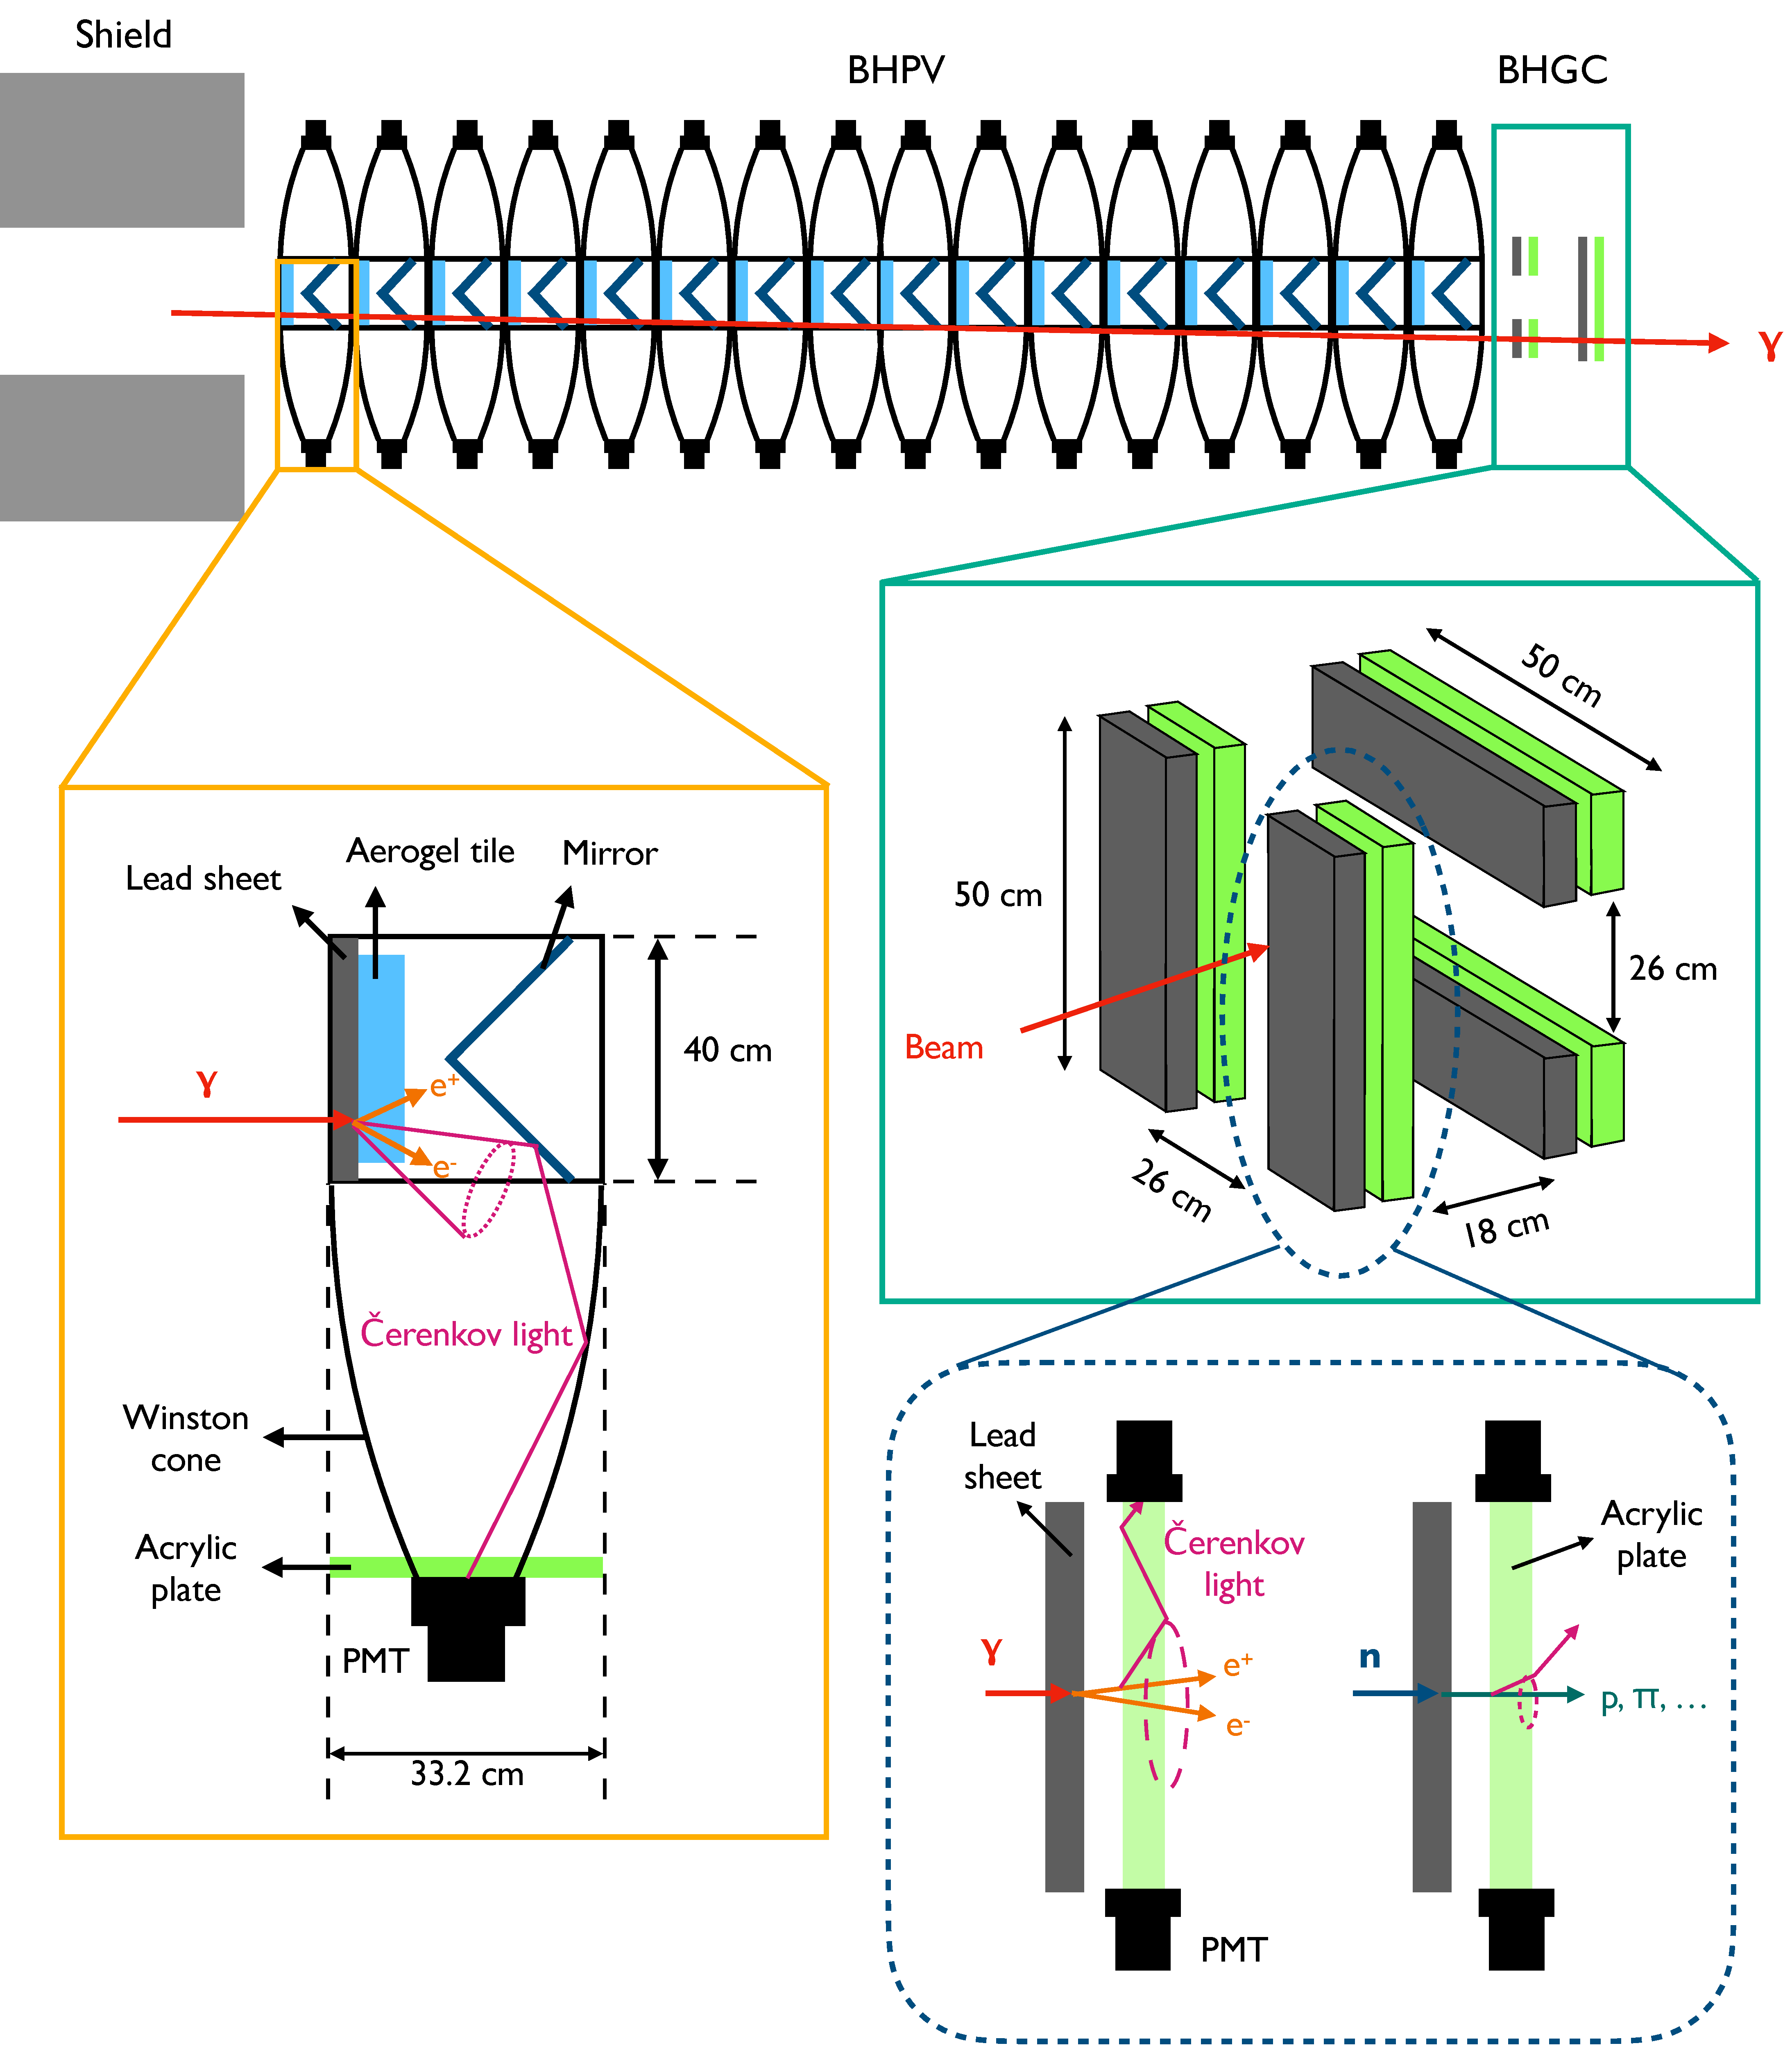
\includegraphics[width=0.9\textwidth]{Figures/Chapter3/BHPV_BHGC.pdf}
%\caption{A graphical illustration of BHPV and BHGC. (Figure courtesy of \parencite{BHPV} with modifications).}
%\label{fig:BHPV_BHGC}
%\end{center}
%\end{figure}

\begin{figure}[h]
\begin{center}
\captionsetup{width=.99\linewidth}
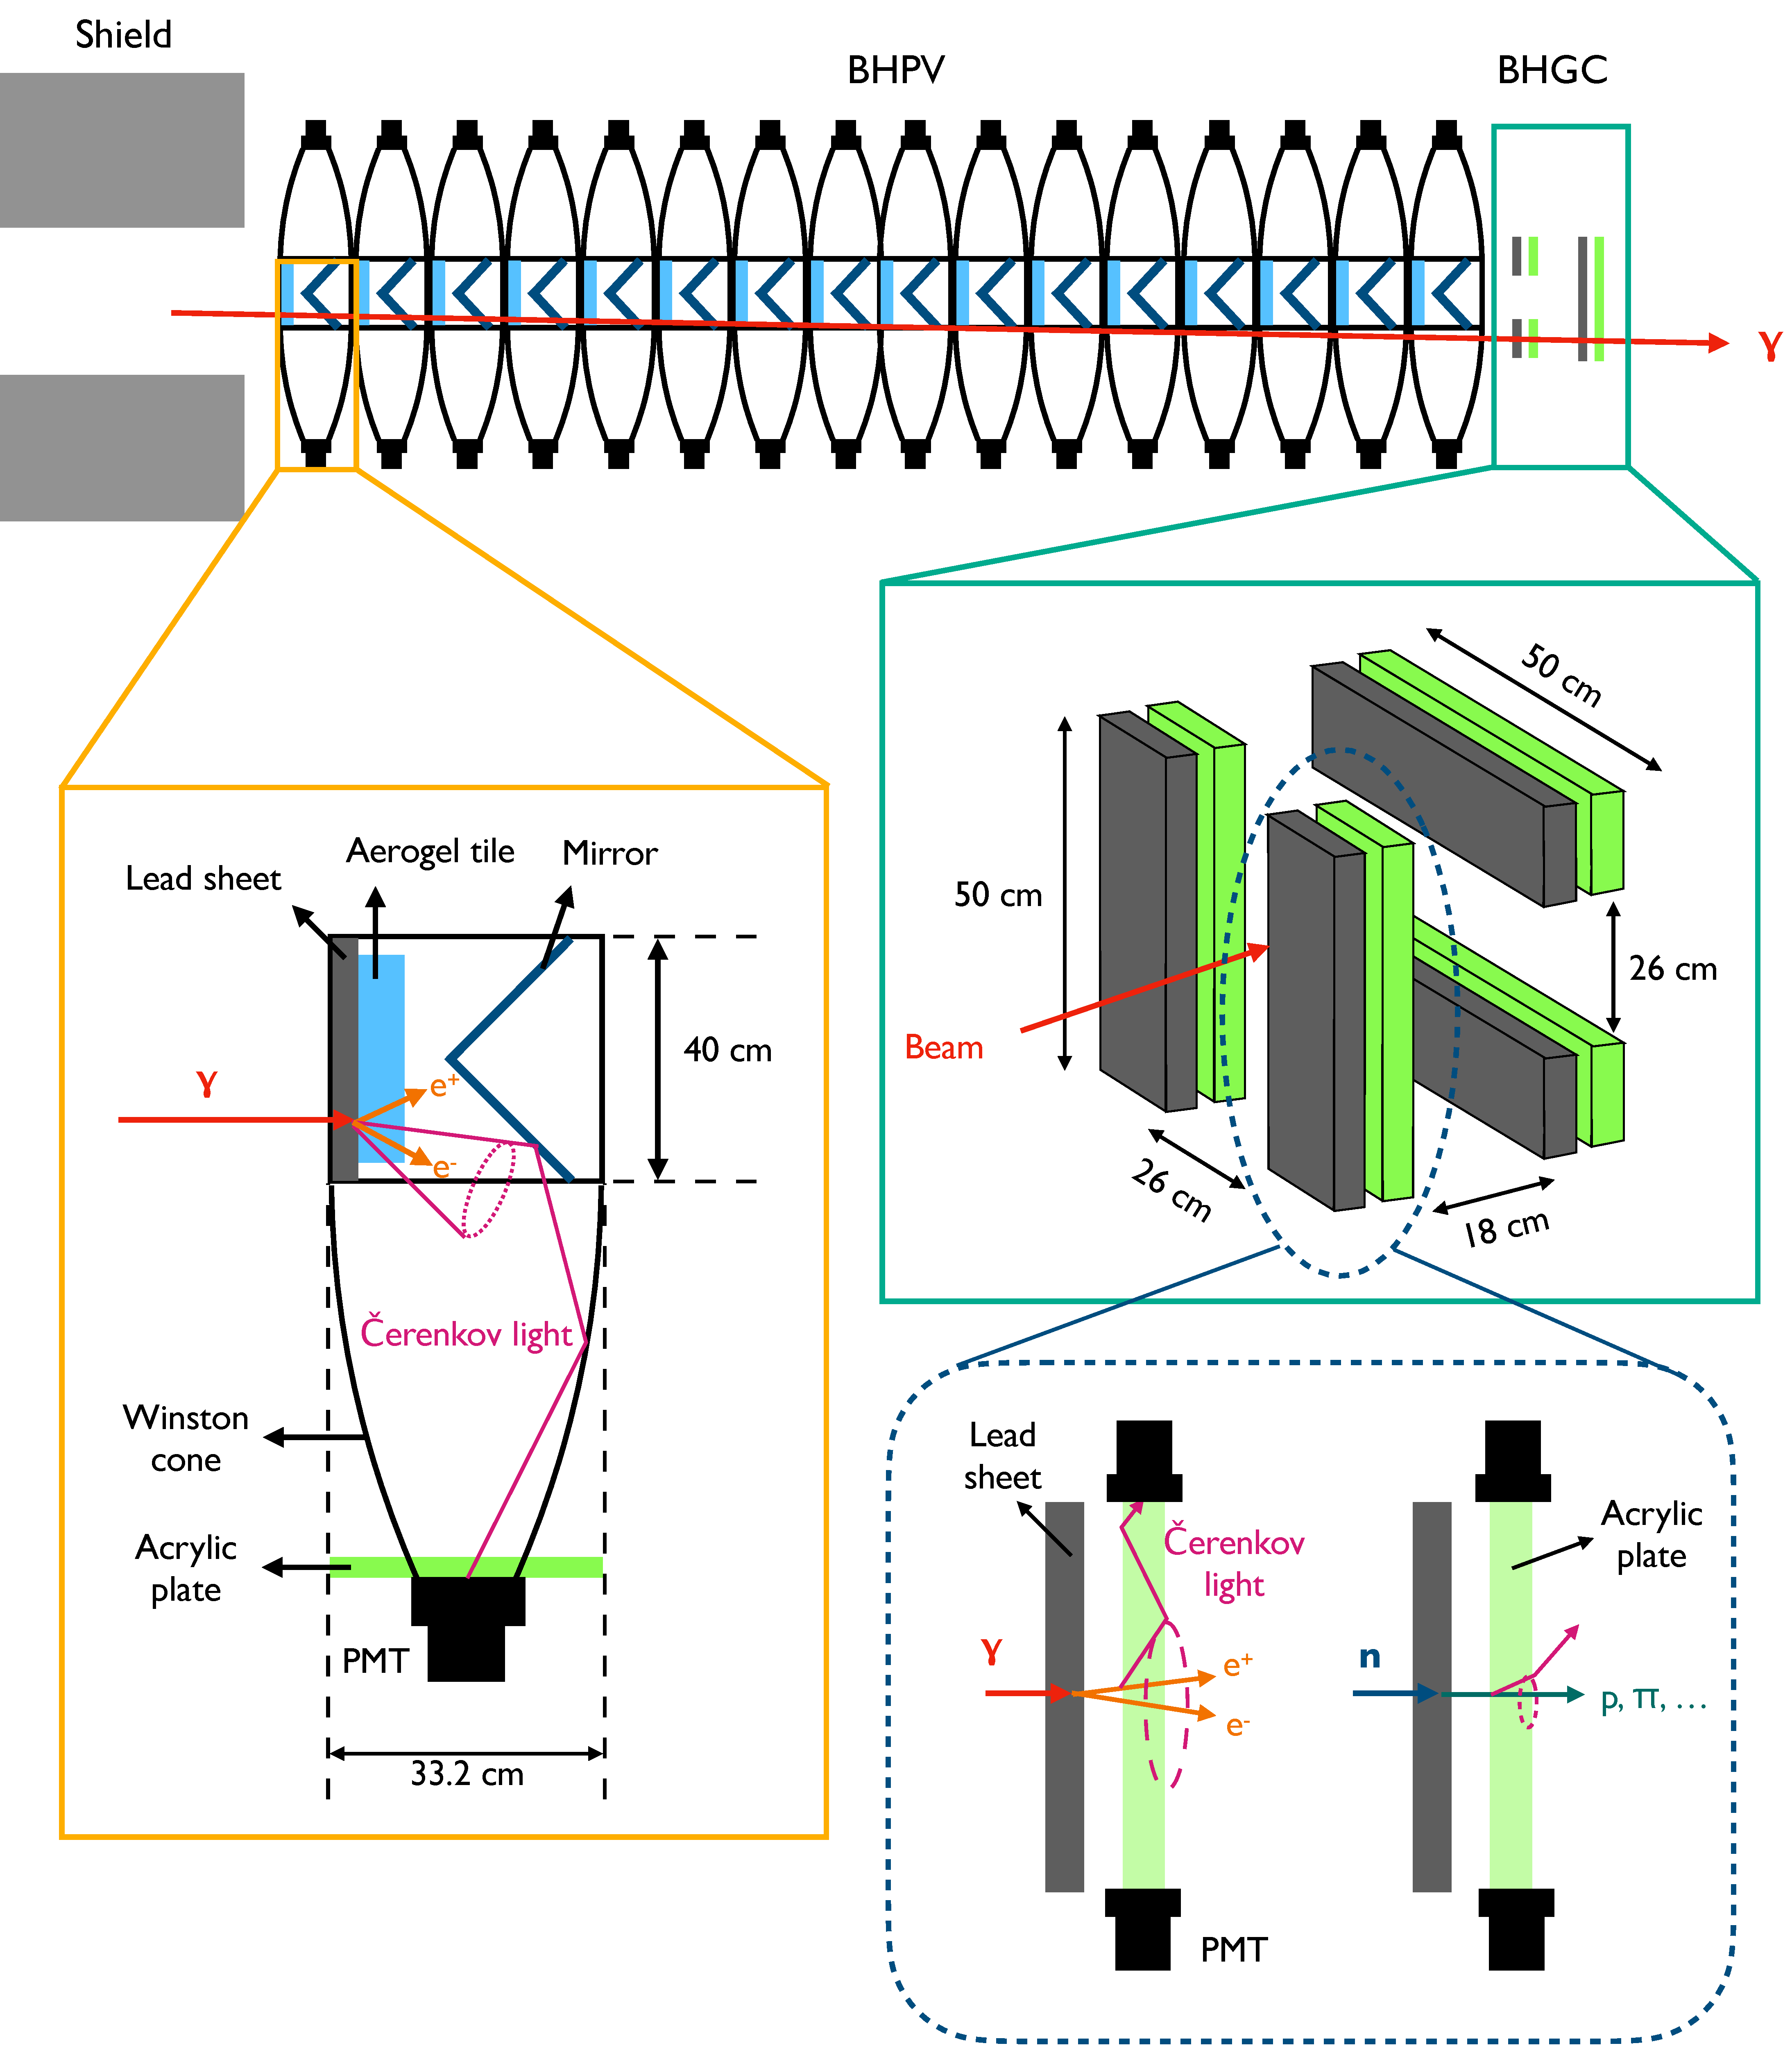
\includegraphics[width=0.99\textwidth]{Figures/Chapter3/BHPV_BHGC.pdf}
\caption{A schematic diagram of BHPV and BHGC \parencite{BHPV, BHGC}.}
\label{fig:BHPV_BHGC}
\end{center}
\end{figure}



% Chapter 3. Design of the KOTO Data-Aqusition System with Cluster-Finding Trigger
% Chapter Template

\chapter{Design of Data-Acquisition System with Cluster-Finding Trigger} % Main chapter title

\label{Chapter4} % Change X to a consecutive number; for referencing this chapter elsewhere, use \ref{ChapterX}

% outline
%----------------------------------------------------------------------------
% 4-1 : Overview of the KOTO DAQ 
% 4-2 : 
% 4-3 : 
% 4-4 : 

A valid physics event, which in general represents a $K_L^0$ decay, contains the hit variables from the entire detector. Those variables are obtained by analyzing the pulses from nearly 4000 channels. Because the $K_L^0$ decay time is not controllable, a methodology needs to be established to record the pulses at the appropriate moment.


the data-acquisition (DAQ) system is supposed to collect the signals from all channels at the suitable moment. Furthermore, due to the hardware limitation, the three-level trigger system is designed to suppress the background-like events and maximally collect the signals under the high-flux beam. 

The KOTO DAQ system had been elaborately upgraded since 2017 to improve the collection efficiency, the rate control, and the flexibility to various physics topics. The overall architecture is explained in this chapter. 

%----------------------------------------------------------------------------------------
%	SECTION 1: Overview of the KOTO DAQ
%----------------------------------------------------------------------------------------

\section{Overview of the KOTO Data-Acquisition System}
The fundamental concept of the KOTO DAQ system is the pipeline readout, as shown in Figure~\ref{fig:pipeline}. The signals from nearly 4000 channels are continuously digitized by the customized flush-analog-to-digital converter (FADC) at either 125 MHz or 500 MHz, and recorded in the memory. The size of the memory for the input data stream corresponds to 5.2~$\SI{}{\mu}$s, known as the pipeline depth, and  



%The memory in the Field Programmable Gate Array (FPGA) on each FADC board keeps updating the input signal within the past 5.2~$\SI{}{\mu}$s, known as the pipeline depth. During this period, the advantageous features are extracted out from the inputs and delivered to the trigger core for further analysis.  


\begin{figure}[h]
\begin{center}
\captionsetup{width=.99\linewidth}
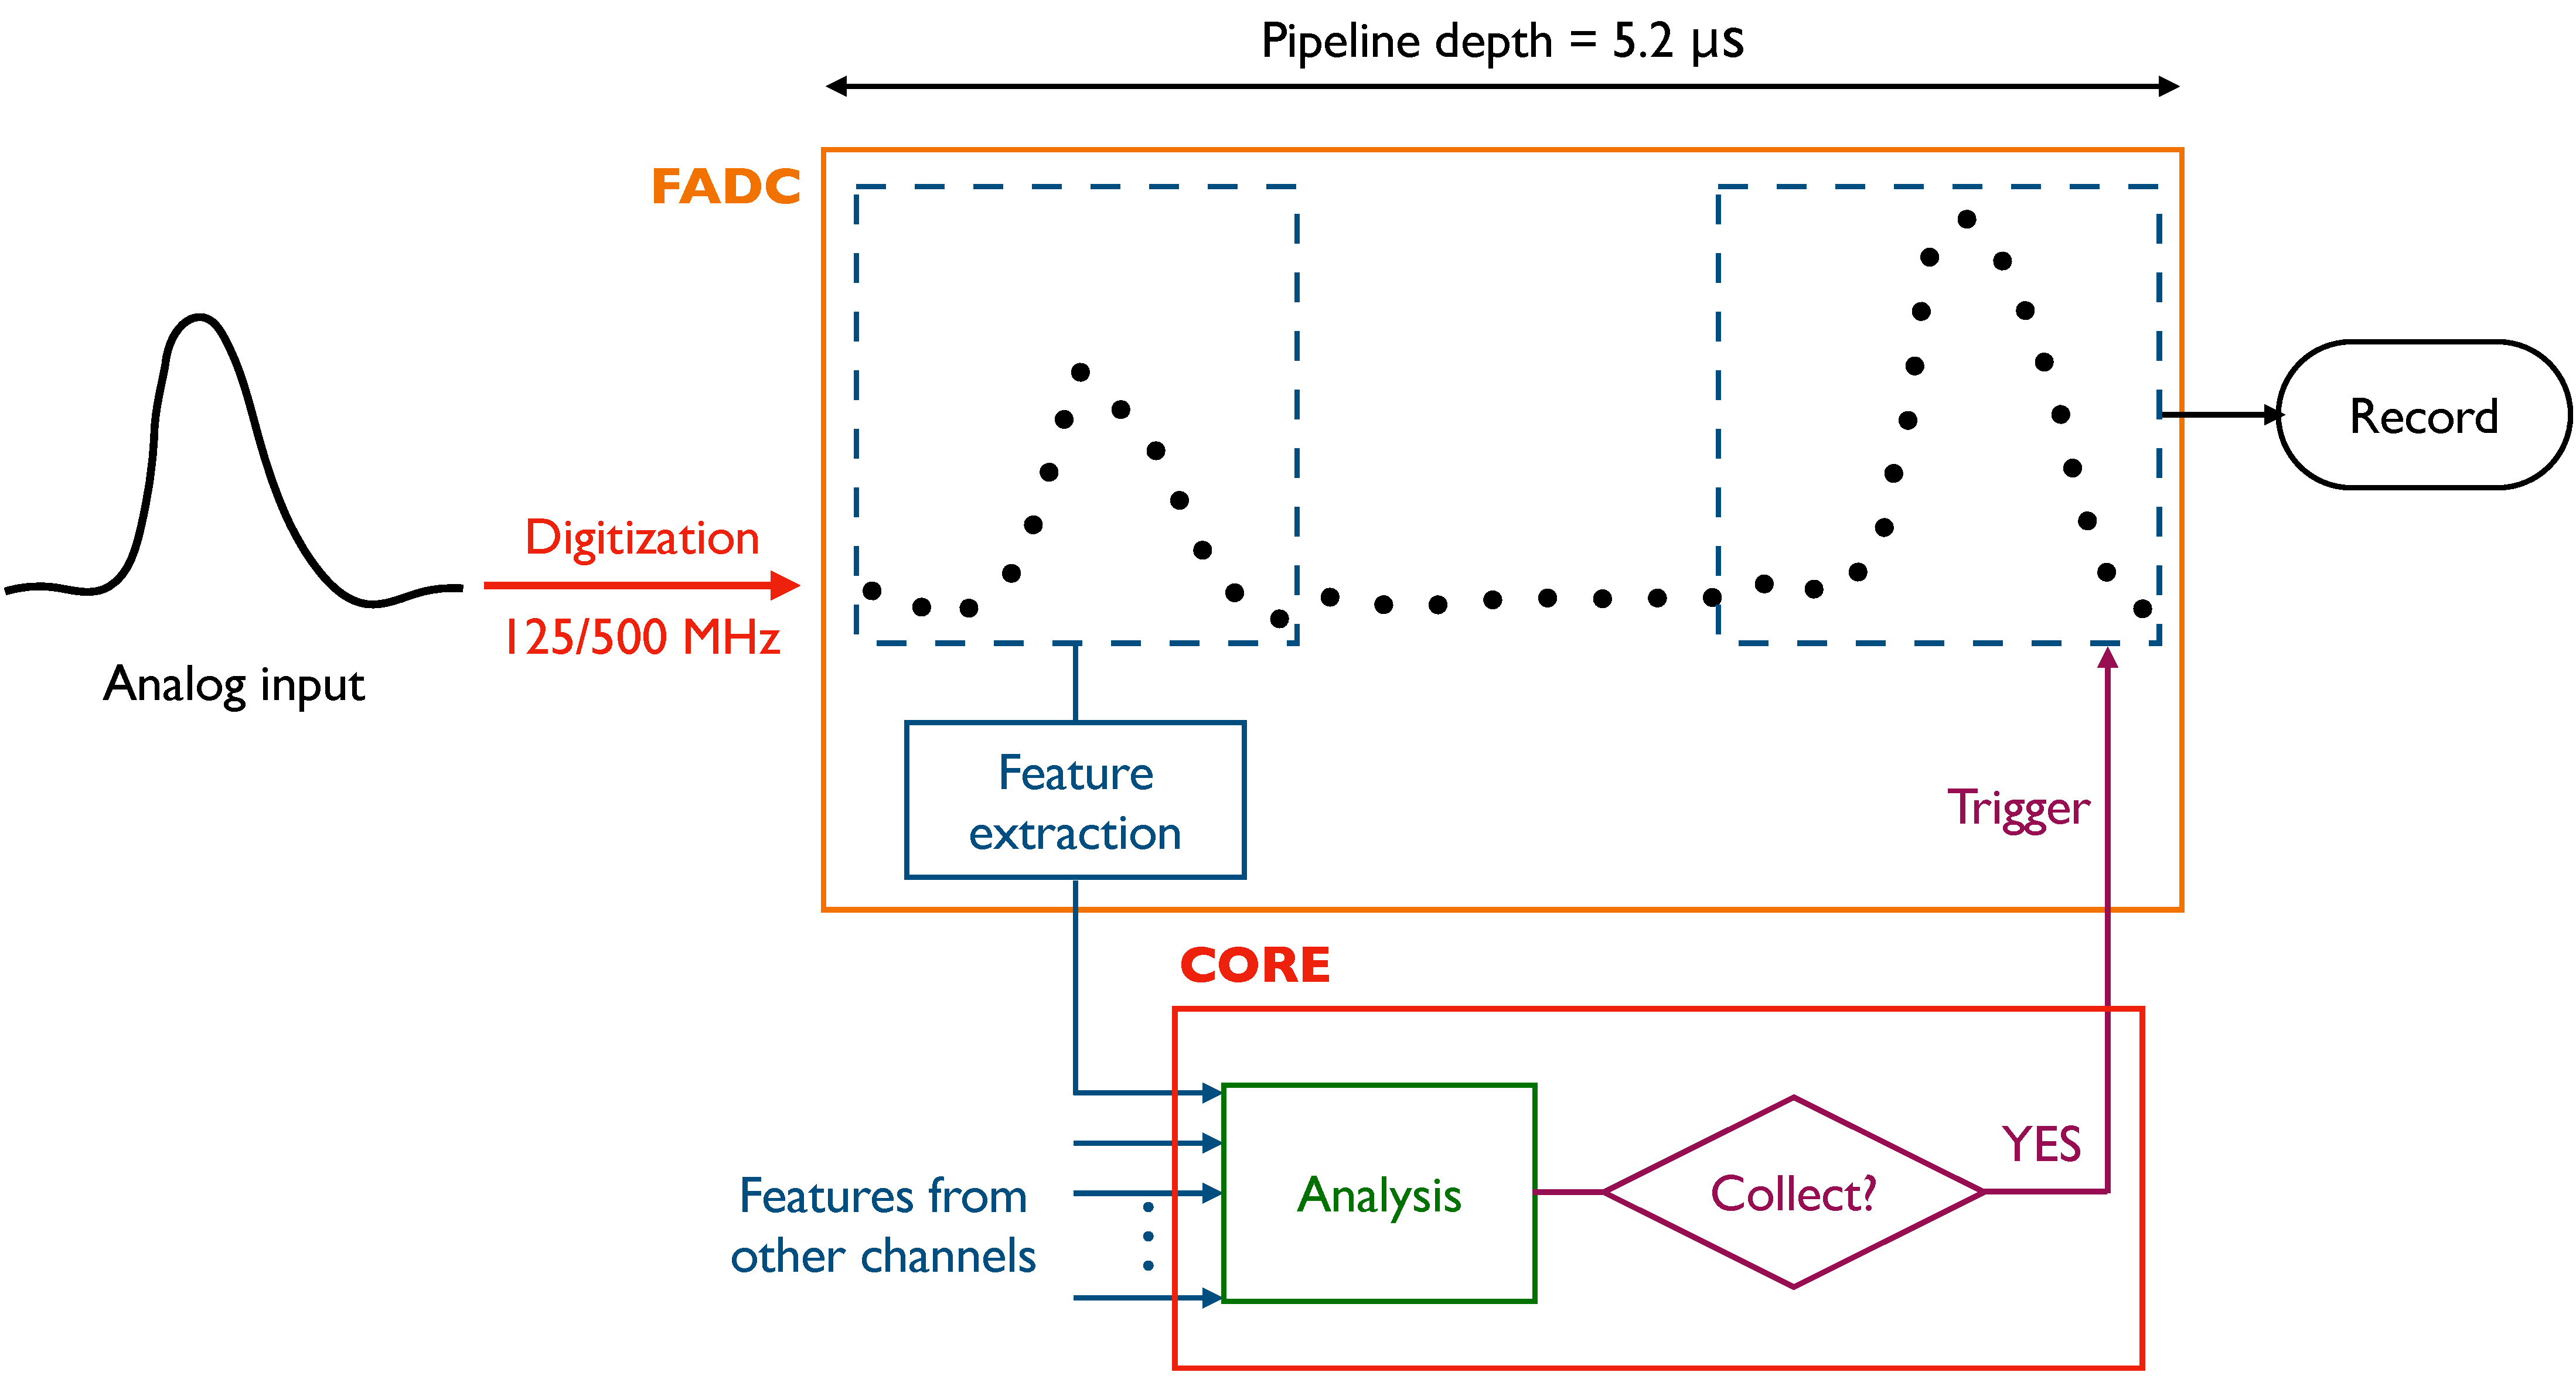
\includegraphics[width=0.99\textwidth]{Figures/Chapter4/pipeline.pdf}
\caption{Fundamental concept of the KOTO trigger. }
\label{fig:pipeline}
\end{center}
\end{figure}


% side caption
%\begin{figure}[h]
% \begin{minipage}[c]{0.5\textwidth}
%    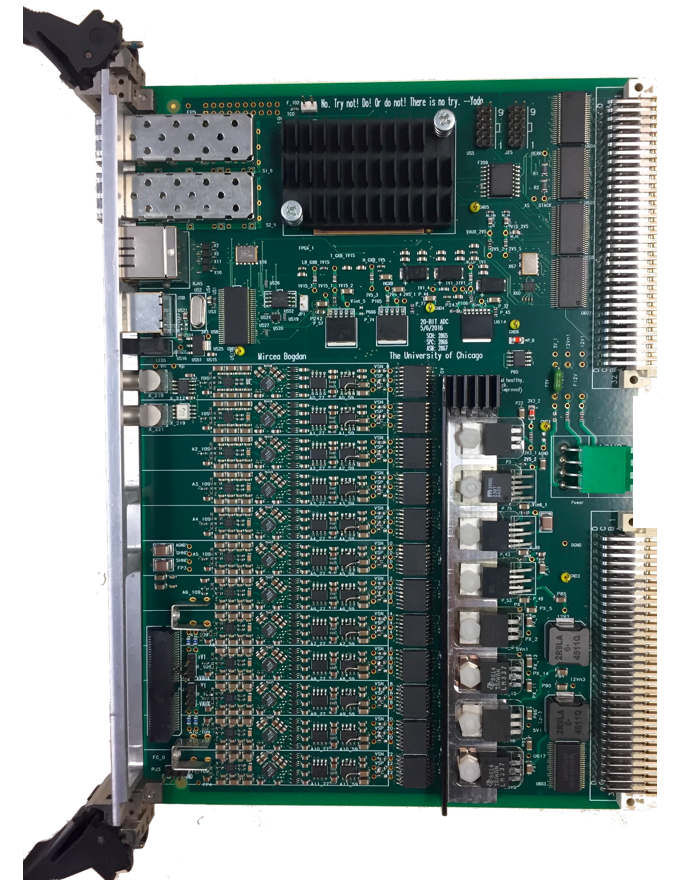
\includegraphics[width=\textwidth]{Figures/Chapter4/ADC.png}
%  \end{minipage}\hfill
%  \begin{minipage}[c]{0.5\textwidth}
%    \captionsetup{width=.99\linewidth}
%    \vspace*{\fill}
%    \caption{
%       A picture of 125-MHz ADC.
%    } \label{fig:ADC_pic}
%  \end{minipage}
%\end{figure}


\section{test}


\parencite{125MHz_ADC}

\begin{figure}[h]
\begin{center}
\captionsetup{width=.99\linewidth}
\includegraphics[width=0.99\textwidth]{Figures/Chapter4/ADC_picture.pdf}
\caption{A picture of a 125-MHz FADC (left) and a 500-MHz FADC (right) board manufactured by University of Chicago  (Figure courtesy of \parencite{mircea}). A 125-MHz (500-MHz) consists of 16 (4) analog inputs, two RJ-45 connectors for LVDS transmission, two optical fiber connectors, and an FPGA of Altera.}
\label{fig:ADC_picture}
\end{center}
\end{figure}


 

% Chapter 4. Observable Extraction
% Chapter Template

\chapter{Observable Extraction} % Main chapter title

\label{Chapter5} % Change X to a consecutive number; for referencing this chapter elsewhere, use \ref{ChapterX}


% 5-1: 125-MHz energy/timing extraction
% 5-2: 500-MHz energy/timing extraction
% 5-3: energy/timing algorithm for calorimeter.
% 5-4: energy/timing algorithm for vetoes.

Energy and timing are the two fundamental observables for physics analysis. When an event is triggered, waveforms from nearly 4000 channels are recorded. 
The algorithm to compute energy and timing is necessary to.

%----------------------------------------------------------------------------------------
%	SECTION 1
%----------------------------------------------------------------------------------------

\section{Energy Extraction}

Lorem ipsum dolor sit amet, consectetur adipiscing elit. Aliquam ultricies lacinia euismod. Nam tempus risus in dolor rhoncus in interdum enim tincidunt. Donec vel nunc neque. In condimentum ullamcorper quam non consequat. Fusce sagittis tempor feugiat. Fusce magna erat, molestie eu convallis ut, tempus sed arcu. Quisque molestie, ante a tincidunt ullamcorper, sapien enim dignissim lacus, in semper nibh erat lobortis purus. Integer dapibus ligula ac risus convallis pellentesque.

%-----------------------------------
%	SUBSECTION 1
%-----------------------------------
\subsection{Subsection 1}

Nunc posuere quam at lectus tristique eu ultrices augue venenatis. Vestibulum ante ipsum primis in faucibus orci luctus et ultrices posuere cubilia Curae; Aliquam erat volutpat. Vivamus sodales tortor eget quam adipiscing in vulputate ante ullamcorper. Sed eros ante, lacinia et sollicitudin et, aliquam sit amet augue. In hac habitasse platea dictumst.

%-----------------------------------
%	SUBSECTION 2
%-----------------------------------

\subsection{Subsection 2}
Morbi rutrum odio eget arcu adipiscing sodales. Aenean et purus a est pulvinar pellentesque. Cras in elit neque, quis varius elit. Phasellus fringilla, nibh eu tempus venenatis, dolor elit posuere quam, quis adipiscing urna leo nec orci. Sed nec nulla auctor odio aliquet consequat. Ut nec nulla in ante ullamcorper aliquam at sed dolor. Phasellus fermentum magna in augue gravida cursus. Cras sed pretium lorem. Pellentesque eget ornare odio. Proin accumsan, massa viverra cursus pharetra, ipsum nisi lobortis velit, a malesuada dolor lorem eu neque.

%----------------------------------------------------------------------------------------
%	SECTION 2
%----------------------------------------------------------------------------------------

\section{Timing C}

Sed ullamcorper quam eu nisl interdum at interdum enim egestas. Aliquam placerat justo sed lectus lobortis ut porta nisl porttitor. Vestibulum mi dolor, lacinia molestie gravida at, tempus vitae ligula. Donec eget quam sapien, in viverra eros. Donec pellentesque justo a massa fringilla non vestibulum metus vestibulum. Vestibulum in orci quis felis tempor lacinia. Vivamus ornare ultrices facilisis. Ut hendrerit volutpat vulputate. Morbi condimentum venenatis augue, id porta ipsum vulputate in. Curabitur luctus tempus justo. Vestibulum risus lectus, adipiscing nec condimentum quis, condimentum nec nisl. Aliquam dictum sagittis velit sed iaculis. Morbi tristique augue sit amet nulla pulvinar id facilisis ligula mollis. Nam elit libero, tincidunt ut aliquam at, molestie in quam. Aenean rhoncus vehicula hendrerit. 

% Chapter 5. Monte Carlo Simulation 
% Chapter Template

\chapter{Monte Carlo Simulation} % Main chapter title

\label{Chapter6} % Change X to a consecutive number; for referencing this chapter elsewhere, use \ref{ChapterX}

%----------------------------------------------------------------------------------------
%	SECTION 1
%----------------------------------------------------------------------------------------

\section{Main Section 1}

Lorem ipsum dolor sit amet, consectetur adipiscing elit. Aliquam ultricies lacinia euismod. Nam tempus risus in dolor rhoncus in interdum enim tincidunt. Donec vel nunc neque. In condimentum ullamcorper quam non consequat. Fusce sagittis tempor feugiat. Fusce magna erat, molestie eu convallis ut, tempus sed arcu. Quisque molestie, ante a tincidunt ullamcorper, sapien enim dignissim lacus, in semper nibh erat lobortis purus. Integer dapibus ligula ac risus convallis pellentesque.

%-----------------------------------
%	SUBSECTION 1
%-----------------------------------
\subsection{Subsection 1}

Nunc posuere quam at lectus tristique eu ultrices augue venenatis. Vestibulum ante ipsum primis in faucibus orci luctus et ultrices posuere cubilia Curae; Aliquam erat volutpat. Vivamus sodales tortor eget quam adipiscing in vulputate ante ullamcorper. Sed eros ante, lacinia et sollicitudin et, aliquam sit amet augue. In hac habitasse platea dictumst.

%-----------------------------------
%	SUBSECTION 2
%-----------------------------------

\subsection{Subsection 2}
Morbi rutrum odio eget arcu adipiscing sodales. Aenean et purus a est pulvinar pellentesque. Cras in elit neque, quis varius elit. Phasellus fringilla, nibh eu tempus venenatis, dolor elit posuere quam, quis adipiscing urna leo nec orci. Sed nec nulla auctor odio aliquet consequat. Ut nec nulla in ante ullamcorper aliquam at sed dolor. Phasellus fermentum magna in augue gravida cursus. Cras sed pretium lorem. Pellentesque eget ornare odio. Proin accumsan, massa viverra cursus pharetra, ipsum nisi lobortis velit, a malesuada dolor lorem eu neque.

%----------------------------------------------------------------------------------------
%	SECTION 2
%----------------------------------------------------------------------------------------

\section{Main Section 2}

Sed ullamcorper quam eu nisl interdum at interdum enim egestas. Aliquam placerat justo sed lectus lobortis ut porta nisl porttitor. Vestibulum mi dolor, lacinia molestie gravida at, tempus vitae ligula. Donec eget quam sapien, in viverra eros. Donec pellentesque justo a massa fringilla non vestibulum metus vestibulum. Vestibulum in orci quis felis tempor lacinia. Vivamus ornare ultrices facilisis. Ut hendrerit volutpat vulputate. Morbi condimentum venenatis augue, id porta ipsum vulputate in. Curabitur luctus tempus justo. Vestibulum risus lectus, adipiscing nec condimentum quis, condimentum nec nisl. Aliquam dictum sagittis velit sed iaculis. Morbi tristique augue sit amet nulla pulvinar id facilisis ligula mollis. Nam elit libero, tincidunt ut aliquam at, molestie in quam. Aenean rhoncus vehicula hendrerit. 

% Chapter 6. Kaon Yield Estimation
% Chapter Template

\chapter{Kaon Yield Estimation} % Main chapter title

\label{Chapter7} % Change X to a consecutive number; for referencing this chapter elsewhere, use \ref{ChapterX}

%----------------------------------------------------------------------------------------
%	SECTION 1
%----------------------------------------------------------------------------------------

\section{Main Section 1}

Lorem ipsum dolor sit amet, consectetur adipiscing elit. Aliquam ultricies lacinia euismod. Nam tempus risus in dolor rhoncus in interdum enim tincidunt. Donec vel nunc neque. In condimentum ullamcorper quam non consequat. Fusce sagittis tempor feugiat. Fusce magna erat, molestie eu convallis ut, tempus sed arcu. Quisque molestie, ante a tincidunt ullamcorper, sapien enim dignissim lacus, in semper nibh erat lobortis purus. Integer dapibus ligula ac risus convallis pellentesque.

%-----------------------------------
%	SUBSECTION 1
%-----------------------------------
\subsection{Subsection 1}

Nunc posuere quam at lectus tristique eu ultrices augue venenatis. Vestibulum ante ipsum primis in faucibus orci luctus et ultrices posuere cubilia Curae; Aliquam erat volutpat. Vivamus sodales tortor eget quam adipiscing in vulputate ante ullamcorper. Sed eros ante, lacinia et sollicitudin et, aliquam sit amet augue. In hac habitasse platea dictumst.

%-----------------------------------
%	SUBSECTION 2
%-----------------------------------

\subsection{Subsection 2}
Morbi rutrum odio eget arcu adipiscing sodales. Aenean et purus a est pulvinar pellentesque. Cras in elit neque, quis varius elit. Phasellus fringilla, nibh eu tempus venenatis, dolor elit posuere quam, quis adipiscing urna leo nec orci. Sed nec nulla auctor odio aliquet consequat. Ut nec nulla in ante ullamcorper aliquam at sed dolor. Phasellus fermentum magna in augue gravida cursus. Cras sed pretium lorem. Pellentesque eget ornare odio. Proin accumsan, massa viverra cursus pharetra, ipsum nisi lobortis velit, a malesuada dolor lorem eu neque.

%----------------------------------------------------------------------------------------
%	SECTION 2
%----------------------------------------------------------------------------------------

\section{Main Section 2}

Sed ullamcorper quam eu nisl interdum at interdum enim egestas. Aliquam placerat justo sed lectus lobortis ut porta nisl porttitor. Vestibulum mi dolor, lacinia molestie gravida at, tempus vitae ligula. Donec eget quam sapien, in viverra eros. Donec pellentesque justo a massa fringilla non vestibulum metus vestibulum. Vestibulum in orci quis felis tempor lacinia. Vivamus ornare ultrices facilisis. Ut hendrerit volutpat vulputate. Morbi condimentum venenatis augue, id porta ipsum vulputate in. Curabitur luctus tempus justo. Vestibulum risus lectus, adipiscing nec condimentum quis, condimentum nec nisl. Aliquam dictum sagittis velit sed iaculis. Morbi tristique augue sit amet nulla pulvinar id facilisis ligula mollis. Nam elit libero, tincidunt ut aliquam at, molestie in quam. Aenean rhoncus vehicula hendrerit. 

% Chapter 7. Evaluation of Trigger Performance
% Chapter Template

\chapter{Evaluation of Trigger Performance} % Main chapter title

\label{Chapter8} % Change X to a consecutive number; for referencing this chapter elsewhere, use \ref{ChapterX}

%----------------------------------------------------------------------------------------
%	SECTION 1
%----------------------------------------------------------------------------------------

\section{Main Section 1}

Lorem ipsum dolor sit amet, consectetur adipiscing elit. Aliquam ultricies lacinia euismod. Nam tempus risus in dolor rhoncus in interdum enim tincidunt. Donec vel nunc neque. In condimentum ullamcorper quam non consequat. Fusce sagittis tempor feugiat. Fusce magna erat, molestie eu convallis ut, tempus sed arcu. Quisque molestie, ante a tincidunt ullamcorper, sapien enim dignissim lacus, in semper nibh erat lobortis purus. Integer dapibus ligula ac risus convallis pellentesque.

%-----------------------------------
%	SUBSECTION 1
%-----------------------------------
\subsection{Subsection 1}

Nunc posuere quam at lectus tristique eu ultrices augue venenatis. Vestibulum ante ipsum primis in faucibus orci luctus et ultrices posuere cubilia Curae; Aliquam erat volutpat. Vivamus sodales tortor eget quam adipiscing in vulputate ante ullamcorper. Sed eros ante, lacinia et sollicitudin et, aliquam sit amet augue. In hac habitasse platea dictumst.

%-----------------------------------
%	SUBSECTION 2
%-----------------------------------

\subsection{Subsection 2}
Morbi rutrum odio eget arcu adipiscing sodales. Aenean et purus a est pulvinar pellentesque. Cras in elit neque, quis varius elit. Phasellus fringilla, nibh eu tempus venenatis, dolor elit posuere quam, quis adipiscing urna leo nec orci. Sed nec nulla auctor odio aliquet consequat. Ut nec nulla in ante ullamcorper aliquam at sed dolor. Phasellus fermentum magna in augue gravida cursus. Cras sed pretium lorem. Pellentesque eget ornare odio. Proin accumsan, massa viverra cursus pharetra, ipsum nisi lobortis velit, a malesuada dolor lorem eu neque.

%----------------------------------------------------------------------------------------
%	SECTION 2
%----------------------------------------------------------------------------------------

\section{Main Section 2}

Sed ullamcorper quam eu nisl interdum at interdum enim egestas. Aliquam placerat justo sed lectus lobortis ut porta nisl porttitor. Vestibulum mi dolor, lacinia molestie gravida at, tempus vitae ligula. Donec eget quam sapien, in viverra eros. Donec pellentesque justo a massa fringilla non vestibulum metus vestibulum. Vestibulum in orci quis felis tempor lacinia. Vivamus ornare ultrices facilisis. Ut hendrerit volutpat vulputate. Morbi condimentum venenatis augue, id porta ipsum vulputate in. Curabitur luctus tempus justo. Vestibulum risus lectus, adipiscing nec condimentum quis, condimentum nec nisl. Aliquam dictum sagittis velit sed iaculis. Morbi tristique augue sit amet nulla pulvinar id facilisis ligula mollis. Nam elit libero, tincidunt ut aliquam at, molestie in quam. Aenean rhoncus vehicula hendrerit. 

% Chapter 8. Analysis of KLpi0nn (KLpi0X, X->invisible)
% Chapter Template

\chapter{Analysis of $K_L^0 \to \pi^0 \nu \bar{\nu}$} % Main chapter title

\label{Chapter9} % Change X to a consecutive number; for referencing this chapter elsewhere, use \ref{ChapterX}

%----------------------------------------------------------------------------------------
%	SECTION 1
%----------------------------------------------------------------------------------------

\section{Main Section 1}

Lorem ipsum dolor sit amet, consectetur adipiscing elit. Aliquam ultricies lacinia euismod. Nam tempus risus in dolor rhoncus in interdum enim tincidunt. Donec vel nunc neque. In condimentum ullamcorper quam non consequat. Fusce sagittis tempor feugiat. Fusce magna erat, molestie eu convallis ut, tempus sed arcu. Quisque molestie, ante a tincidunt ullamcorper, sapien enim dignissim lacus, in semper nibh erat lobortis purus. Integer dapibus ligula ac risus convallis pellentesque.

%-----------------------------------
%	SUBSECTION 1
%-----------------------------------
\subsection{Subsection 1}

Nunc posuere quam at lectus tristique eu ultrices augue venenatis. Vestibulum ante ipsum primis in faucibus orci luctus et ultrices posuere cubilia Curae; Aliquam erat volutpat. Vivamus sodales tortor eget quam adipiscing in vulputate ante ullamcorper. Sed eros ante, lacinia et sollicitudin et, aliquam sit amet augue. In hac habitasse platea dictumst.

%-----------------------------------
%	SUBSECTION 2
%-----------------------------------

\subsection{Subsection 2}
Morbi rutrum odio eget arcu adipiscing sodales. Aenean et purus a est pulvinar pellentesque. Cras in elit neque, quis varius elit. Phasellus fringilla, nibh eu tempus venenatis, dolor elit posuere quam, quis adipiscing urna leo nec orci. Sed nec nulla auctor odio aliquet consequat. Ut nec nulla in ante ullamcorper aliquam at sed dolor. Phasellus fermentum magna in augue gravida cursus. Cras sed pretium lorem. Pellentesque eget ornare odio. Proin accumsan, massa viverra cursus pharetra, ipsum nisi lobortis velit, a malesuada dolor lorem eu neque.

%----------------------------------------------------------------------------------------
%	SECTION 2
%----------------------------------------------------------------------------------------

\section{Main Section 2}

Sed ullamcorper quam eu nisl interdum at interdum enim egestas. Aliquam placerat justo sed lectus lobortis ut porta nisl porttitor. Vestibulum mi dolor, lacinia molestie gravida at, tempus vitae ligula. Donec eget quam sapien, in viverra eros. Donec pellentesque justo a massa fringilla non vestibulum metus vestibulum. Vestibulum in orci quis felis tempor lacinia. Vivamus ornare ultrices facilisis. Ut hendrerit volutpat vulputate. Morbi condimentum venenatis augue, id porta ipsum vulputate in. Curabitur luctus tempus justo. Vestibulum risus lectus, adipiscing nec condimentum quis, condimentum nec nisl. Aliquam dictum sagittis velit sed iaculis. Morbi tristique augue sit amet nulla pulvinar id facilisis ligula mollis. Nam elit libero, tincidunt ut aliquam at, molestie in quam. Aenean rhoncus vehicula hendrerit. 

% Chapter 9. Analysis of KLpi0gg 
% Chapter Template

\chapter{Analysis of $K_L^0 \to \pi^0 \gamma \gamma$} % Main chapter title

\label{Chapter10} % Change X to a consecutive number; for referencing this chapter elsewhere, use \ref{ChapterX}

%----------------------------------------------------------------------------------------
%	SECTION 1
%----------------------------------------------------------------------------------------

\section{Main Section 1}

Lorem ipsum dolor sit amet, consectetur adipiscing elit. Aliquam ultricies lacinia euismod. Nam tempus risus in dolor rhoncus in interdum enim tincidunt. Donec vel nunc neque. In condimentum ullamcorper quam non consequat. Fusce sagittis tempor feugiat. Fusce magna erat, molestie eu convallis ut, tempus sed arcu. Quisque molestie, ante a tincidunt ullamcorper, sapien enim dignissim lacus, in semper nibh erat lobortis purus. Integer dapibus ligula ac risus convallis pellentesque.

%-----------------------------------
%	SUBSECTION 1
%-----------------------------------
\subsection{Subsection 1}

Nunc posuere quam at lectus tristique eu ultrices augue venenatis. Vestibulum ante ipsum primis in faucibus orci luctus et ultrices posuere cubilia Curae; Aliquam erat volutpat. Vivamus sodales tortor eget quam adipiscing in vulputate ante ullamcorper. Sed eros ante, lacinia et sollicitudin et, aliquam sit amet augue. In hac habitasse platea dictumst.

%-----------------------------------
%	SUBSECTION 2
%-----------------------------------

\subsection{Subsection 2}
Morbi rutrum odio eget arcu adipiscing sodales. Aenean et purus a est pulvinar pellentesque. Cras in elit neque, quis varius elit. Phasellus fringilla, nibh eu tempus venenatis, dolor elit posuere quam, quis adipiscing urna leo nec orci. Sed nec nulla auctor odio aliquet consequat. Ut nec nulla in ante ullamcorper aliquam at sed dolor. Phasellus fermentum magna in augue gravida cursus. Cras sed pretium lorem. Pellentesque eget ornare odio. Proin accumsan, massa viverra cursus pharetra, ipsum nisi lobortis velit, a malesuada dolor lorem eu neque.

%----------------------------------------------------------------------------------------
%	SECTION 2
%----------------------------------------------------------------------------------------

\section{Main Section 2}

Sed ullamcorper quam eu nisl interdum at interdum enim egestas. Aliquam placerat justo sed lectus lobortis ut porta nisl porttitor. Vestibulum mi dolor, lacinia molestie gravida at, tempus vitae ligula. Donec eget quam sapien, in viverra eros. Donec pellentesque justo a massa fringilla non vestibulum metus vestibulum. Vestibulum in orci quis felis tempor lacinia. Vivamus ornare ultrices facilisis. Ut hendrerit volutpat vulputate. Morbi condimentum venenatis augue, id porta ipsum vulputate in. Curabitur luctus tempus justo. Vestibulum risus lectus, adipiscing nec condimentum quis, condimentum nec nisl. Aliquam dictum sagittis velit sed iaculis. Morbi tristique augue sit amet nulla pulvinar id facilisis ligula mollis. Nam elit libero, tincidunt ut aliquam at, molestie in quam. Aenean rhoncus vehicula hendrerit. 

% Chapter 10. Discussion
% Chapter Template

\chapter{Discussion} % Main chapter title

\label{Chapter11} % Change X to a consecutive number; for referencing this chapter elsewhere, use \ref{ChapterX}

%----------------------------------------------------------------------------------------
%	SECTION 1
%----------------------------------------------------------------------------------------

\section{Main Section 1}

Lorem ipsum dolor sit amet, consectetur adipiscing elit. Aliquam ultricies lacinia euismod. Nam tempus risus in dolor rhoncus in interdum enim tincidunt. Donec vel nunc neque. In condimentum ullamcorper quam non consequat. Fusce sagittis tempor feugiat. Fusce magna erat, molestie eu convallis ut, tempus sed arcu. Quisque molestie, ante a tincidunt ullamcorper, sapien enim dignissim lacus, in semper nibh erat lobortis purus. Integer dapibus ligula ac risus convallis pellentesque.

%-----------------------------------
%	SUBSECTION 1
%-----------------------------------
\subsection{Subsection 1}

Nunc posuere quam at lectus tristique eu ultrices augue venenatis. Vestibulum ante ipsum primis in faucibus orci luctus et ultrices posuere cubilia Curae; Aliquam erat volutpat. Vivamus sodales tortor eget quam adipiscing in vulputate ante ullamcorper. Sed eros ante, lacinia et sollicitudin et, aliquam sit amet augue. In hac habitasse platea dictumst.

%-----------------------------------
%	SUBSECTION 2
%-----------------------------------

\subsection{Subsection 2}
Morbi rutrum odio eget arcu adipiscing sodales. Aenean et purus a est pulvinar pellentesque. Cras in elit neque, quis varius elit. Phasellus fringilla, nibh eu tempus venenatis, dolor elit posuere quam, quis adipiscing urna leo nec orci. Sed nec nulla auctor odio aliquet consequat. Ut nec nulla in ante ullamcorper aliquam at sed dolor. Phasellus fermentum magna in augue gravida cursus. Cras sed pretium lorem. Pellentesque eget ornare odio. Proin accumsan, massa viverra cursus pharetra, ipsum nisi lobortis velit, a malesuada dolor lorem eu neque.

%----------------------------------------------------------------------------------------
%	SECTION 2
%----------------------------------------------------------------------------------------

\section{Main Section 2}

Sed ullamcorper quam eu nisl interdum at interdum enim egestas. Aliquam placerat justo sed lectus lobortis ut porta nisl porttitor. Vestibulum mi dolor, lacinia molestie gravida at, tempus vitae ligula. Donec eget quam sapien, in viverra eros. Donec pellentesque justo a massa fringilla non vestibulum metus vestibulum. Vestibulum in orci quis felis tempor lacinia. Vivamus ornare ultrices facilisis. Ut hendrerit volutpat vulputate. Morbi condimentum venenatis augue, id porta ipsum vulputate in. Curabitur luctus tempus justo. Vestibulum risus lectus, adipiscing nec condimentum quis, condimentum nec nisl. Aliquam dictum sagittis velit sed iaculis. Morbi tristique augue sit amet nulla pulvinar id facilisis ligula mollis. Nam elit libero, tincidunt ut aliquam at, molestie in quam. Aenean rhoncus vehicula hendrerit. 

% Chapter 11. Conclusion
% Chapter Template

\chapter{Conclusion} % Main chapter title

\label{Chapter12} % Change X to a consecutive number; for referencing this chapter elsewhere, use \ref{ChapterX}

%----------------------------------------------------------------------------------------
%	SECTION 1
%----------------------------------------------------------------------------------------

\section{Main Section 1}

Lorem ipsum dolor sit amet, consectetur adipiscing elit. Aliquam ultricies lacinia euismod. Nam tempus risus in dolor rhoncus in interdum enim tincidunt. Donec vel nunc neque. In condimentum ullamcorper quam non consequat. Fusce sagittis tempor feugiat. Fusce magna erat, molestie eu convallis ut, tempus sed arcu. Quisque molestie, ante a tincidunt ullamcorper, sapien enim dignissim lacus, in semper nibh erat lobortis purus. Integer dapibus ligula ac risus convallis pellentesque.

%-----------------------------------
%	SUBSECTION 1
%-----------------------------------
\subsection{Subsection 1}

Nunc posuere quam at lectus tristique eu ultrices augue venenatis. Vestibulum ante ipsum primis in faucibus orci luctus et ultrices posuere cubilia Curae; Aliquam erat volutpat. Vivamus sodales tortor eget quam adipiscing in vulputate ante ullamcorper. Sed eros ante, lacinia et sollicitudin et, aliquam sit amet augue. In hac habitasse platea dictumst.

%-----------------------------------
%	SUBSECTION 2
%-----------------------------------

\subsection{Subsection 2}
Morbi rutrum odio eget arcu adipiscing sodales. Aenean et purus a est pulvinar pellentesque. Cras in elit neque, quis varius elit. Phasellus fringilla, nibh eu tempus venenatis, dolor elit posuere quam, quis adipiscing urna leo nec orci. Sed nec nulla auctor odio aliquet consequat. Ut nec nulla in ante ullamcorper aliquam at sed dolor. Phasellus fermentum magna in augue gravida cursus. Cras sed pretium lorem. Pellentesque eget ornare odio. Proin accumsan, massa viverra cursus pharetra, ipsum nisi lobortis velit, a malesuada dolor lorem eu neque.

%----------------------------------------------------------------------------------------
%	SECTION 2
%----------------------------------------------------------------------------------------

\section{Main Section 2}

Sed ullamcorper quam eu nisl interdum at interdum enim egestas. Aliquam placerat justo sed lectus lobortis ut porta nisl porttitor. Vestibulum mi dolor, lacinia molestie gravida at, tempus vitae ligula. Donec eget quam sapien, in viverra eros. Donec pellentesque justo a massa fringilla non vestibulum metus vestibulum. Vestibulum in orci quis felis tempor lacinia. Vivamus ornare ultrices facilisis. Ut hendrerit volutpat vulputate. Morbi condimentum venenatis augue, id porta ipsum vulputate in. Curabitur luctus tempus justo. Vestibulum risus lectus, adipiscing nec condimentum quis, condimentum nec nisl. Aliquam dictum sagittis velit sed iaculis. Morbi tristique augue sit amet nulla pulvinar id facilisis ligula mollis. Nam elit libero, tincidunt ut aliquam at, molestie in quam. Aenean rhoncus vehicula hendrerit. 

%----------------------------------------------------------------------------------------
%	THESIS CONTENT - APPENDICES
%----------------------------------------------------------------------------------------

\appendix % Cue to tell LaTeX that the following "chapters" are Appendices

% Include the appendices of the thesis as separate files from the Appendices folder

% A. Evolution of KOTO DAQ system
\include{Appendices/AppendixB}

% A. Firmware logic (details) / UI / diagnose / monitor tool
%% Appendix A

\chapter{Diagnosis Tool of the KOTO Trigger System} % Main appendix title

\label{AppendixA} % For referencing this appendix elsewhere, use \ref{AppendixA}

\section{Diagnosis Tool of the KOTO Trigger System}
test



The color of links can be changed to your liking using:

{\small\verb!\hypersetup{urlcolor=red}!}, or

{\small\verb!\hypersetup{citecolor=green}!}, or

{\small\verb!\hypersetup{allcolor=blue}!}.

\noindent If you want to completely hide the links, you can use:

{\small\verb!\hypersetup{allcolors=.}!}, or even better: 

{\small\verb!\hypersetup{hidelinks}!}.

\noindent If you want to have obvious links in the PDF but not the printed text, use:

{\small\verb!\hypersetup{colorlinks=false}!}.


% B. Waveform Corruption

% C. Dead channel effect / low gain chaanel  (+noisy channel impact on CDT)

% D. 3rd order spline interpolation for data-based waveform

% E. Double pulse discrimination (Fourier Transform)
% (relative phase issues, the interpretation of transformatition)

% F. TMVA, Machine Learning Algorithm for  (CNN/DL)

% G. T0 correction / LED / LASER

% H. Statistical Implication

% I. gallery (DAQ)

% J. glossary of KOTO

% K. Publication List

% Publication List
%% Appendix X

\chapter{Publication List} % Main appendix title

\label{AppendixX} % For referencing this appendix elsewhere, use \ref{AppendixA}

\nocite{*}
\printbibliography[keyword={my_journal},title={Journal}]
%\printbibliography[keyword={proceeding},title={Conference Proceeding}]


%----------------------------------------------------------------------------------------
%	BIBLIOGRAPHY
%----------------------------------------------------------------------------------------

\printbibliography[heading=bibintoc]


%----------------------------------------------------------------------------------------
%	INDEX
%----------------------------------------------------------------------------------------


\printindex

%----------------------------------------------------------------------------------------

\end{document}  
